\documentclass{report}

% --- Idioma y codificación ---
\usepackage[spanish]{babel}
\usepackage[utf8]{inputenc}
\usepackage[T1]{fontenc}

% --- Página ---
\usepackage[letterpaper,top=2cm,bottom=2cm,left=3cm,right=3cm,marginparwidth=1.75cm]{geometry}
\usepackage{setspace}
\usepackage{fancyhdr}

% --- Matemáticas ---
\usepackage{amsmath}
\usepackage{amssymb}

% --- Tablas y figuras ---
\usepackage{graphicx}
\usepackage{booktabs}      % \toprule, \midrule, \bottomrule
\usepackage{tabularx}
\usepackage{diagbox}
\usepackage{float}
\usepackage[labelfont=bf]{caption}   % numeración + "Tabla X.Y" en negrita
\usepackage{pgfgantt}      % si incluyes el Gantt directamente aquí

% --- Algoritmos ---
\usepackage{algorithm}
\usepackage{algpseudocode}

% --- Listas ---
\usepackage{enumitem}

% --- Color (si lo usas en el cuerpo, no solo en el Gantt standalone) ---
\usepackage{xcolor}

% --- Otros ---
\usepackage{blindtext}
\usepackage[colorlinks=true, allcolors=blue]{hyperref}

% --- Nombres en español ---
\addto\captionsspanish{%
  \renewcommand{\tablename}{Tabla}
  \renewcommand{\figurename}{Figura}
}


\title{Detección de anomalías e imputación en línea de datos corruptos en sistemas de monitoreo continuo de glucosa mediante redes
neuronales profundas y variables fisiológicas}
\author{Daniel Alexander Pascoe Gonzalez}

\begin{document}
\begin{center}
%\vspace*{-3.5cm}
\thispagestyle{empty}
  {\Large \textbf{UNIVERSIDAD DE GUADALAJARA}}\\
  \vspace{0.25cm}
  {\large Centro Universitario de Ciencias Exactas e Ingenierías}\\
  \vspace{0.25cm}
  {\large División de Tecnologías para la Integración Ciber-Humana}\\

  
  
  \begin{figure} [H]
	\begin{center}
	
\includegraphics[width=0.3\textwidth]{udgb (1).png}
	\end{center}
  \end{figure}
  \vspace{0.25cm}
  {\large \textbf{Detección de anomalías e imputación en línea de datos corruptos en sistemas de monitoreo continuo de glucosa mediante redes
neuronales profundas y variables fisiológicas}}\\
  \vspace{0.25cm}
  \vspace{0.25cm}
 
TESIS \\
\vspace{0.25cm}
MAESTRÍA EN CIENCIAS EN ROBÓTICA E INTELIGENCIA ARTIFICIAL\\
\vspace{0.25cm}
\textbf{PRESENTA:}\\
\vspace{0.25cm}
{\large \textbf{Daniel Alexander Pascoe Gonzalez}}\\
{\large \textbf{224809986}}\\
\vspace{0.25cm}
DIRECTOR DE TESIS\\
\vspace{0.25cm}
{\large \textbf{Dr. Oscar Didier Sánchez Sánchez}}\\
\vspace{0.25cm}
CO-DIRECTOR DE TESIS\\
\vspace{0.25cm}
{\large \textbf{Dr. Alma Yolanda Alanís García}}\\

\vspace{0.25cm}
\vspace{0.5cm}
\large {Guadalajara, Jalisco, 20 de Marzo del 2026} \vspace{1cm} \\
\begin{tabular}{p{4cm}p{8cm}}
\end{tabular}
\end{center}

\newpage


\newpage

\chapter*{Resumen}
Aquí va el resumen de la tesis.

\chapter*{Abstract}
One of the main challenges when working with time series captured online using sensors is the appearance of noise or null values, generally caused by sensor failures or temporary disconnections. These errors compromise data reliability and can lead to incorrect decisions. Particularly in the treatment of diabetes mellitus, where medical decisions depend on continuous glucose monitoring (CGM) systems provided by modern sensors, the presence of corrupted data can pose a significant risk to patient health. This work presents an approach that encompasses online detection and imputation of anomalous data using physiological inputs (insulin and carbohydrate intake), which enables decision-making in automatic glucose monitoring systems or for glucose control purposes. Four deep neural network architectures are proposed: CNN-LSTM, GRU, 1D-CNN, and Transformer-LSTM, under a controlled fault injection protocol and compared with the ARIMA model and the Temporal Convolutional Network (TCN). The obtained performance is compared using regression (MAE, RMSE, MARD) and classification (accuracy, precision, recall, F1-score, AUC) metrics. Results show that the CNN-LSTM network is the most effective for fault detection, achieving an F1-score of 0.876 and an accuracy of 0.979. Regarding data imputation, the 1D-CNN network obtained the best performance, with an MAE of 2.96 mg/dL and an RMSE of 3.75 mg/dL. Then, validation on the OhioT1DM dataset, containing real CGM data with natural sensor disconnections, showed that the CNN–LSTM model accurately detected anomalies and reliably imputed missing glucose segments under real-world conditions.

% Para que estos capítulos sin número aparezcan en el índice:
\addcontentsline{toc}{chapter}{Resumen}
\addcontentsline{toc}{chapter}{Abstract}

% ----------------- ÍNDICE AUTOMÁTICO ------------
\tableofcontents
\cleardoublepage

% =================================================
% CAPÍTULO 1. INTRODUCCIÓN
% =================================================
\chapter{Introducción}

\section{Contexto general del problema}
\label{sec:contexto_general}

La diabetes mellitus tipo 1 (DT1) resulta de la destrucción autoinmune de las células $\beta$ del páncreas, lo que suprime la producción endógena de insulina y obliga a quienes la padecen a depender de su administración exógena durante el resto de la vida. Ajustar esa dosis exige conocer con precisión la concentración de glucosa en cada momento, una tarea que durante décadas dependió de mediciones capilares esporádicas, incapaces de seguir la dinámica real de la glucemia entre una punción y la siguiente.

Los sistemas de monitoreo continuo de glucosa (CGM) cambiaron ese panorama al estimar la glucosa intersticial cada pocos minutos y ofrecer así una trayectoria casi continua de la variable~\cite{cobelli2009diabetes}. Esta resolución temporal habilita decisiones que antes eran impracticables: anticipar una hipoglucemia antes de que se manifieste, ajustar la insulina en función de la tendencia y no solo del valor puntual, o alimentar algoritmos de control en lazo cerrado que automatizan parte de la dosificación, un escenario en el que detectar los fallos del sensor se vuelve una condición de seguridad tan relevante como la propia lógica de control~\cite{sanchez2025imputation}. El consenso internacional de la American Diabetes Association (ADA) y la European Association for the Study of Diabetes (EASD) formalizó en 2019 un conjunto de métricas —tiempo en rango, tiempo por debajo y por encima del rango, variabilidad glucémica— que hoy orientan tanto la práctica clínica como la evaluación de nuevos algoritmos de control~\cite{battelino2019}. Todas ellas comparten un supuesto que rara vez se hace explícito: que la señal reportada por el sensor refleja fielmente la glucosa real del paciente.

Ese supuesto falla con más frecuencia de la deseada. Un sensor de CGM puede interrumpir la transmisión durante horas, o bien continuar transmitiendo valores contaminados por ruido electrónico, interferencia electromagnética o el desplazamiento leve de la interfaz con el tejido subcutáneo. Cuando cualquiera de estos fallos pasa inadvertido, contamina tanto la interpretación clínica del paciente como los algoritmos automáticos que dependen de la señal, y lo hace justo en los instantes —cambios rápidos de glucosa, desconexiones prolongadas— en los que una decisión errónea resulta más costosa. Detectar estos fallos en línea y reconstruir la señal con un criterio fisiológicamente coherente termina siendo, por ello, una condición tan relevante para la seguridad del paciente como la exactitud misma del sensor.

\section{Planteamiento del problema de investigación}
\label{sec:planteamiento_problema}

Frente al problema descrito en la Sección~\ref{sec:contexto_general}, la literatura ha comenzado a explorar sistemas de detección e imputación en línea basados en redes neuronales profundas que combinan la señal de glucosa con variables fisiológicas de entrada, como la insulina administrada y los carbohidratos ingeridos. El trabajo previo del grupo de investigación~\cite{sanchez2025imputation} constituye, dentro de esa línea, un antecedente directo: compara cuatro arquitecturas —CNN-LSTM, GRU, 1D-CNN y Transformer-LSTM— bajo un protocolo de inyección controlada de fallos y reporta, para la mejor configuración, un F1-score superior a 0.87 en la detección y un error medio absoluto de imputación por debajo de 3~mg/dL. Estos resultados confirman que el enfoque es viable, pero dejan también expuestas tres limitaciones que esta tesis toma como punto de partida.

Primero, la decisión de marcar una lectura como fallo se apoya en un umbral fijo de 10~mg/dL, idéntico para cualquier nivel de glucosa y cualquier velocidad de cambio de la señal. Un umbral constante no distingue, sin embargo, dos fuentes de variación bien documentadas: la norma ISO 15197~\cite{iso15197_2013} establece tolerancias distintas para la hipoglucemia y para el resto del rango glucémico, y las predicciones de la red se degradan de forma transitoria durante una excursión posprandial rápida, exista o no un fallo real del sensor. Segundo, la misma arquitectura que genera la predicción usada para detectar el fallo produce también el valor de reemplazo cuando este ocurre, aunque detectar y reconstruir sean tareas de naturaleza distinta —clasificación en un caso, regresión en el otro— que no necesariamente favorecen a la misma red. La validación sobre datos clínicos reales, en tercer lugar, se limitó a un único paciente del conjunto OhioT1DM y se reportó solo en términos de métricas de clasificación, sin conectar los resultados con los indicadores clínicos estandarizados que en la práctica determinan si un sistema de este tipo es útil para el manejo de la diabetes.

Estas limitaciones acotan el problema que esta tesis aborda: establecer si el esquema de detección e imputación en línea puede extenderse en tres direcciones —dotar al umbral de decisión de una dependencia explícita del contexto glucémico, separar la detección y la imputación en arquitecturas seleccionadas de forma independiente para cada tarea, y ampliar la validación sobre datos reales hasta un punto en el que sea posible reportar indicadores clínicos estandarizados— sin sacrificar el desempeño ya demostrado por el sistema del que parte. Los Capítulos 3 y 4 desarrollan y evalúan, respectivamente, la propuesta y sus resultados.


\section{Justificación}
\label{sec:justificacion}

Un sistema que detecte fallos del sensor y reconstruya la señal de CGM en línea no es un ejercicio exclusivamente técnico: la calidad de esa señal condiciona decisiones terapéuticas que se toman varias veces al día, desde la dosis de insulina hasta la respuesta ante una alerta de hipoglucemia. Un falso negativo en la detección —un fallo que pasa como lectura válida— puede traducirse en una decisión clínica tomada sobre datos erróneos. Un falso positivo, en cambio, sustituye una lectura genuina por una predicción del modelo y descarta información real del paciente. Ambos errores tienen costo clínico, y ese costo justifica por sí solo dedicar un esfuerzo de investigación a reducirlos.

A esa motivación clínica se suma una carencia identificable en el estado del arte: como se discutió en la Sección~\ref{sec:planteamiento_problema}, pocos trabajos integran detección de fallos e imputación en un mismo esquema apoyado en variables fisiológicas, y menos todavía evalúan ese esquema bajo un umbral adaptado al contexto glucémico o con arquitecturas especializadas por tarea. Cerrar esa carencia, incluso de forma parcial, amplía lo que se sabe sobre cómo estructurar sistemas de este tipo para su eventual uso en dispositivos comerciales o en algoritmos de control en lazo cerrado.

La factibilidad del proyecto, por su parte, no depende únicamente de argumentos teóricos. El grupo de investigación cuenta con una base de código validada y con datos simulados y reales previamente procesados, producto del trabajo publicado en~\cite{sanchez2025imputation}, cuyas métricas de detección y de imputación superaron de manera consistente a los métodos de referencia considerados en ese mismo estudio (ARIMA y una red convolucional temporal). Partir de una infraestructura que ya demostró ese desempeño reduce el riesgo técnico del proyecto y permite concentrar el esfuerzo de esta tesis en las tres extensiones descritas en la Sección~\ref{sec:planteamiento_problema}, en lugar de reconstruir el sistema desde cero.


\section{Hipótesis}
\label{sec:hipotesis}

La hipótesis de este trabajo es que sustituir el umbral fijo de detección por uno que se adapte al contexto glucémico, y evaluar de manera independiente las combinaciones posibles entre detector e imputador, produce un sistema de detección e imputación en línea con mejor desempeño técnico que el esquema unificado y de umbral fijo del trabajo previo: menos falsos positivos en la detección de fallos y una reconstrucción de la señal más precisa.

Se espera también que esta mejora técnica no se quede en las métricas de señal. Al evaluar el sistema propuesto sobre un conjunto más amplio de pacientes reales de OhioT1DM, y no solo sobre el paciente único que consideró el trabajo previo, los indicadores clínicos de control glucémico --tiempo en rango, variabilidad, riesgo de hipo o hiperglucemia-- deberían reflejar una ganancia consistente con la mejora observada a nivel de señal.

\section{Objetivos}
\label{sec:objetivos}

\subsection{Objetivo General}
\label{subsec:objetivo_general}

Desarrollar y validar un sistema de detección de fallos e imputación en línea para señales de monitoreo continuo de glucosa, basado en redes neuronales profundas que integran como entradas la glucosa histórica, la insulina administrada y los carbohidratos ingeridos, con el fin de mejorar la confiabilidad de la señal reportada y, con ello, la seguridad de las decisiones terapéuticas que dependen de ella en personas con DT1.


\subsection{Objetivos Específicos}
\begin{itemize}
    \item Implementar y entrenar las cuatro arquitecturas profundas (CNN-LSTM, GRU, 1D-CNN y Transformer-LSTM) empleadas como base para las tareas de detección de fallos e imputación, verificando la estabilidad de su desempeño frente a distintas inicializaciones.

    \item Diseñar y validar un umbral de detección adaptativo al contexto glucémico, y comparar su desempeño frente al umbral fijo utilizado en el trabajo previo.

    \item Evaluar de forma desacoplada las combinaciones posibles entre detector e imputador, para determinar si ambas tareas pueden optimizarse de manera independiente e identificar así la configuración global más adecuada.

    \item Cuantificar el impacto clínico del sistema propuesto mediante indicadores de control glucémico --tiempo en rango, variabilidad y GMI-- sobre datos simulados, y extender esa evaluación a datos reales del conjunto OhioT1DM.
\end{itemize}

\section{Alcances y limitaciones}
\label{sec:alcances_limitaciones}

La validación experimental de este trabajo se hizo en dos etapas. En la primera se usaron datos sintéticos generados con el modelo fisiológico de Sorensen, sobre los cuales se probaron de forma exhaustiva el umbral adaptativo y el pipeline desacoplado, en un entorno donde los escenarios de fallo se controlan por diseño. En la segunda etapa se llevó el sistema resultante --ya con los parámetros fijados en la primera-- a datos reales del conjunto OhioT1DM, donde las fallas de sensor ocurren de forma natural y no se pueden ajustar a conveniencia. Este orden implica que la calibración del sistema se hizo sobre la señal sintética, y que su capacidad de generalizar a datos reales es, en sí misma, parte de lo que se evalúa en la segunda etapa y no algo que se dé por sentado.

Las cuatro arquitecturas evaluadas --CNN-LSTM, GRU, 1D-CNN y Transformer-LSTM-- son las mismas del trabajo previo del grupo, con capas e hiperparámetros de entrenamiento idénticos. Esta tesis no explora arquitecturas nuevas: la variable de interés es el esquema de detección e imputación --fijo frente a adaptativo, unificado frente a desacoplado-- y modificar al mismo tiempo las arquitecturas impediría atribuir con claridad las diferencias de desempeño a una sola causa. Los parámetros del umbral
adaptativo se mantuvieron iguales para las cuatro, priorizando una configuración unificada sobre un ajuste fino por arquitectura.

A esta validación se suma una restricción propia del conjunto OhioT1DM: al no incluir una traza de glucosa de referencia, la evaluación sobre datos reales se limita a métricas de clasificación y a una revisión cualitativa de la imputación, sin que sea posible reportar ahí un error de reconstrucción en mg/dL como sí ocurre con los datos sintéticos.

Quedan fuera del alcance de esta tesis la implementación del sistema en un dispositivo embebido y su integración en un lazo de control de insulina en tiempo real. Ambos puntos son relevantes para llevar este trabajo a unescenario clínico o comercial, pero requieren un desarrollo de ingeniería y una validación regulatoria que corresponden a una etapa posterior, no a esta tesis.

% =================================================
% CAPÍTULO 2. MARCO TEÓRICO Y ESTADO DEL ARTE
% =================================================
\chapter{Marco Teórico y Estado del Arte}

\section{Diabetes mellitus tipo 1 y sistemas CGM}

\section{Fallos en sensores y datos faltantes en series temporales multivariadas}

%% 2.4
\section{Métodos tradicionales de imputación y sus limitaciones}


\section{Redes neuronales profundas para series temporales} % (del paper, sec. 3)
\label{sec:redes_neuronales_profundas}

En esta sección se introducen las arquitecturas de aprendizaje profundo empleadas para la imputación en línea de datos corruptos en sensores de CGM. Específicamente, se presentan los modelos basados en LSTM, GRU, 1D-CNN y Transformer. Para cada arquitectura se describen sus principios de operación, las formulaciones matemáticas centrales y su relevancia para la imputación de datos de CGM en tiempo real.

\subsection{Long Short-Term Memory (LSTM)}
\label{subsec:lstm}
Las redes LSTM son una variante especializada de las redes neuronales recurrentes (RNN) diseñadas para capturar dependencias temporales tanto de corto como de largo plazo en datos secuenciales. A diferencia de las RNN convencionales, que suelen verse afectadas por el problema del desvanecimiento del gradiente, las LSTM introducen una celda de memoria regulada por tres compuertas —de entrada, de olvido y de salida— que controlan el flujo de información a lo largo del tiempo. Estos mecanismos determinan qué información se conserva, se actualiza o se descarta, permitiendo que la red mantenga un contexto relevante a través de secuencias extensas~\cite{siami2019performance}.

Formalmente, las operaciones dentro de una celda LSTM se describen mediante las siguientes ecuaciones~\cite{siami2019performance, sanchez2023realtime}:

\begin{equation}
\label{eq:lstm}
\begin{aligned}
f_t &= \sigma(W_{fh} h_{t-1} + W_{fx} x_t + b_f) \\
i_t &= \sigma(W_{ih} h_{t-1} + W_{ix} x_t + b_i) \\
\tilde{c}_t &= \tanh(W_{ch} h_{t-1} + W_{cx} x_t + b_c) \\
c_t &= f_t \cdot c_{t-1} + i_t \cdot \tilde{c}_t \\
o_t &= \sigma(W_{oh} h_{t-1} + W_{ox} x_t + b_o) \\
h_t &= o_t \cdot \tanh(c_t)
\end{aligned}
\end{equation}

Aquí, $x_t \in \mathbb{R}^{n_x}$ es el vector de entrada en el instante $t$ (información de glucosa, insulina e ingesta de alimentos), $h_{t-1} \in \mathbb{R}^{n_h}$ es el estado oculto anterior y $c_{t-1} \in \mathbb{R}^{n_h}$ el estado anterior de la celda. Las matrices $W_{\cdot h} \in \mathbb{R}^{n_h \times n_h}$ y $W_{\cdot x} \in \mathbb{R}^{n_h \times n_x}$ son matrices de pesos, y $b_{\cdot} \in \mathbb{R}^{n_h}$ son los vectores de sesgo asociados a cada compuerta. La activación logística $\sigma(\cdot)$ mapea valores al intervalo $[0, 1]$, controlando la activación de las compuertas, mientras que $\tanh(\cdot)$ proporciona transformaciones no lineales acotadas. La compuerta de olvido $f_t$ escala la memoria previa, la compuerta de entrada $i_t$ controla cómo se incorpora la nueva información $\tilde{c}_t$, y la compuerta de salida $o_t$ determina qué proporción de la memoria actualizada $c_t$ contribuye al nuevo estado oculto $h_t$.

Estos mecanismos permiten a las redes LSTM retener información relevante a lo largo de horizontes temporales prolongados, lo cual resulta particularmente valioso para modelar sistemas no lineales y variantes en el tiempo, como las señales fisiológicas. En este contexto, las LSTM son especialmente efectivas para capturar los efectos retardados de la absorción de insulina o la digestión prolongada de los alimentos, manteniendo la estabilidad durante interrupciones extendidas, ventaja que justifica su mayor costo computacional. Además, estudios previos han demostrado que el uso de curvas intermedias de absorción para insulina y carbohidratos simplifica el proceso de aprendizaje en los modelos recurrentes, mejorando la precisión predictiva al alinear la representación de entrada con la dinámica fisiológica subyacente~\cite{lindemann2020survey, munoz2021learning}.

\subsection{Gated Recurrent Units (GRU)}
\label{subsec:gru}
Las GRU son una variante simplificada de las redes LSTM, diseñadas para reducir la complejidad computacional sin perder la capacidad de capturar dependencias temporales. Fusionan las compuertas de entrada y de olvido en una única compuerta de actualización e introducen una compuerta de reinicio para controlar el flujo de información~\cite{dey2017gate}. Esta estructura disminuye el número de parámetros y mejora la eficiencia computacional.

Las operaciones de una celda GRU se definen como~\cite{dey2017gate}:

\begin{equation}
\label{eq:gru}
\begin{aligned}
z_t &= \sigma(W_{xz} x_t + W_{hz} h_{t-1} + b_z) \\
r_t &= \sigma(W_{xr} x_t + W_{hr} h_{t-1} + b_r) \\
\tilde{h}_t &= \tanh(W_{xh} x_t + W_{hh} (r_t \odot h_{t-1}) + b_h) \\
h_t &= (1 - z_t) \odot h_{t-1} + z_t \odot \tilde{h}_t
\end{aligned}
\end{equation}

Aquí, $x_t \in \mathbb{R}^{n_x}$ es el vector de entrada en el instante $t$, $h_t \in \mathbb{R}^{n_h}$ es el estado oculto y $\tilde{h}_t$ denota la activación candidata. Las matrices $W_{x\{z,r,h\}} \in \mathbb{R}^{n_h \times n_x}$ corresponden a los pesos asociados a la entrada, mientras que $W_{h\{z,r,h\}} \in \mathbb{R}^{n_h \times n_h}$ representan los pesos recurrentes conectados al estado oculto previo $h_{t-1} \in \mathbb{R}^{n_h}$. Los vectores $b_z, b_r, b_h \in \mathbb{R}^{n_h}$ son los términos de sesgo. Las funciones de activación $\sigma(\cdot)$ y $\tanh(\cdot)$ denotan la sigmoide y la tangente hiperbólica, respectivamente, y el producto de Hadamard ($\odot$) indica multiplicación elemento a elemento.

La compuerta de actualización $z_t$ determina qué cantidad de la memoria previa se conserva, mientras que la compuerta de reinicio $r_t$ controla cuánta información pasada se ignora al calcular la activación candidata $\tilde{h}_t$. Mediante la combinación de estos dos mecanismos, las GRU modelan eficazmente dependencias de largo plazo con menos parámetros y una convergencia más rápida que las LSTM, ofreciendo un equilibrio práctico entre precisión y eficiencia.

En este trabajo, la arquitectura GRU se implementó como una alternativa recurrente computacionalmente eficiente para la imputación en línea y la detección de fallos en datos de monitoreo continuo de glucosa (CGM). Estudios previos han mostrado que las GRU pueden alcanzar valores de RMSE más bajos y un menor sobreajuste en comparación con las LSTM y las RNN convencionales~\cite{siami2019performance, alshehri2024blood}. Su mecanismo compacto de compuertas permite un aprendizaje estable de las dependencias temporales en señales fisiológicas como la glucosa, la insulina y la ingesta de alimentos, logrando un compromiso efectivo entre precisión predictiva y latencia en tiempo real.

\subsection{Redes Neuronales Convolucionales 1D (1D-CNN)}
\label{subsec:1dcnn}
A través de operaciones de convolución, las redes 1D-CNN capturan de forma eficiente patrones locales y temporales en datos secuenciales. Están conformadas por capas convolucionales que aplican filtros (\textit{kernels}) sobre ventanas deslizantes de las secuencias de entrada para extraer características de alto nivel relevantes para tareas de predicción~\cite{li2019convolutional, Shenfield2020rolling}. Formalmente, una convolución unidimensional se define como:

\begin{equation}
\label{eq:conv1d}
y_j^{(l)} = f\!\left( \sum_{i=0}^{k-1} w_i^{(l)}\, x_{j+i}^{(l-1)} + b^{(l)} \right),
\end{equation}

donde $y_j^{(l)}$ es la salida en la posición $j$ de la capa $l$, $w_i^{(l)}$ son los pesos del filtro, $x_{j+i}^{(l-1)}$ son las entradas provenientes de la capa anterior, $b^{(l)}$ es el término de sesgo, $k$ es el tamaño del \textit{kernel} y $f(\cdot)$ es una función de activación no lineal, típicamente ReLU. La Figura~\ref{fig:1dcnn} ilustra una arquitectura general de 1D-CNN con bloques Conv1D--\textit{pooling} para series temporales multivariadas.

 \begin{figure}[h]
     \centering
     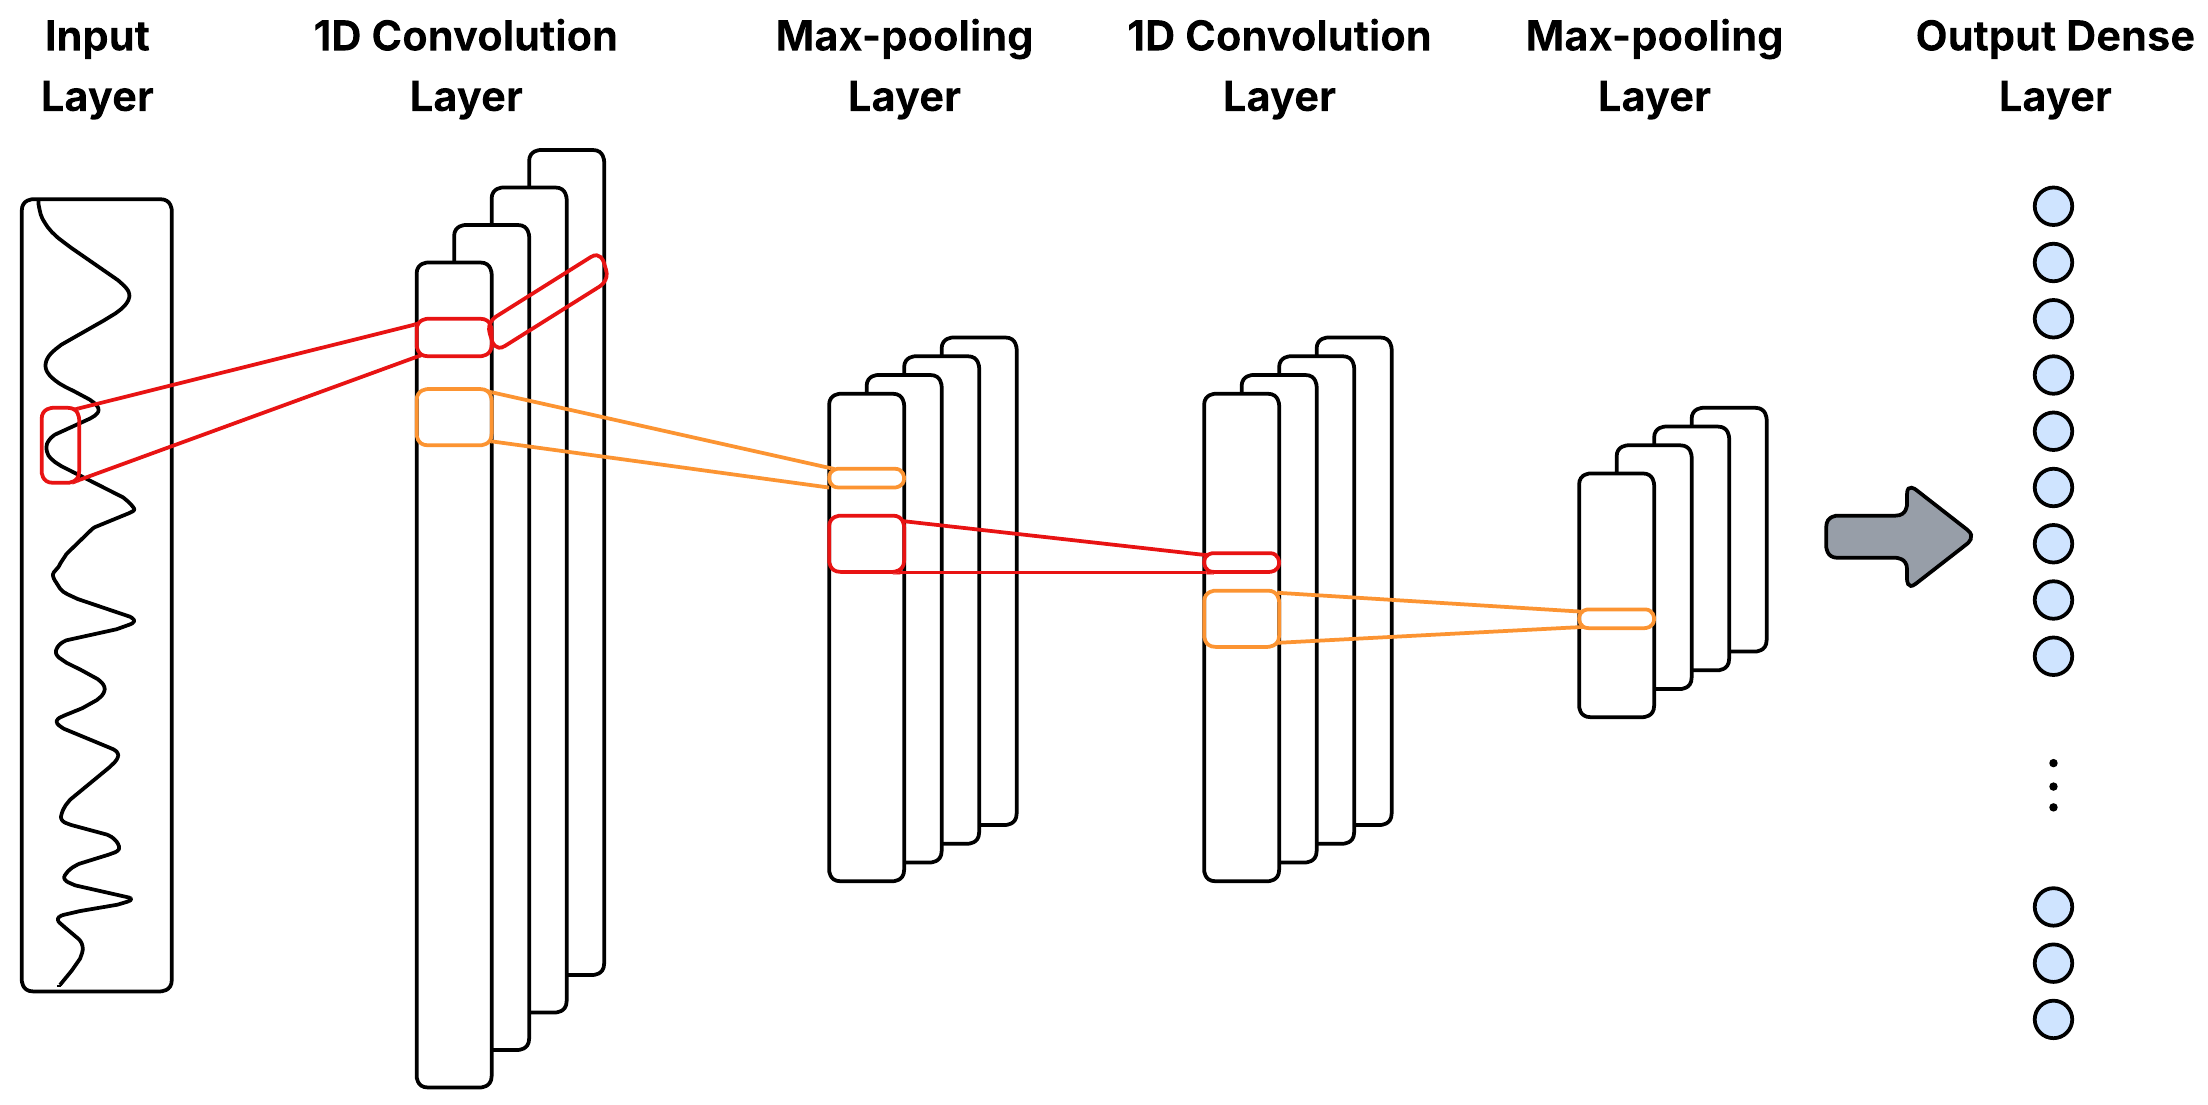
\includegraphics[width=0.9\textwidth]{figures/1D-CNN-Diagram-Pooling.png}
     \caption{Arquitectura general de una 1D-CNN con bloques Conv1D--\textit{pooling} para series temporales multivariadas.}
     \label{fig:1dcnn}
 \end{figure}

Las capas de \textit{pooling} reducen la dimensionalidad de los mapas de características al resumir vecindarios temporales pequeños, mediante \textit{max-pooling} o \textit{average-pooling}, de modo que la representación preserva las características salientes mientras se reduce la resolución. En datos de series temporales, el \textit{pooling} introduce una invariancia limitada a pequeños desplazamientos temporales, suprime el ruido de alta frecuencia mediante agregación local y disminuye el número de activaciones que se transmiten a las capas más profundas, mejorando tanto la generalización como la eficiencia computacional~\cite{Zhou2022WRR_FloodInundation_DL}.

Adicionalmente, las 1D-CNN son robustas frente al ruido y eficaces para reconocer patrones temporales dentro de segmentos cortos de datos, lo que las hace particularmente adecuadas para el preprocesamiento de señales CGM ruidosas o intermitentes antes de su análisis por modelos recurrentes o basados en atención~\cite{alkanhel2024hybrid}. Estudios recientes también han demostrado que los modelos híbridos que combinan CNN con capas recurrentes, como las GRU, pueden mejorar aún más la precisión en la predicción de glucosa en sangre, evidenciando su potencial para aplicaciones de manejo de la diabetes en tiempo real~\cite{alkanhel2024hybrid}.

\subsection{Modelos Basados en Transformers}
\label{subsec:transformer}

Los modelos basados en Transformer se han vuelto cada vez más populares para la predicción de series temporales debido a su capacidad de modelar dependencias de largo alcance sin recurrencia. Estos modelos se apoyan en un mecanismo de auto-atención que pondera dinámicamente la relevancia de los distintos elementos de la secuencia. La operación central es la atención por producto punto escalado:

\begin{equation}
\label{eq:attention}
\mathrm{Attention}(Q, K, V) = \mathrm{softmax}\!\left( \frac{Q K^{T}}{\sqrt{d_k}} \right) V,
\end{equation}

donde $Q$, $K$ y $V$ son las matrices de consulta (\textit{query}), clave (\textit{key}) y valor (\textit{value}), y $d_k$ es la dimensión de la clave. La atención multi-cabeza extiende este mecanismo como:

\begin{equation}
\label{eq:multihead}
\mathrm{MultiHead}(Q, K, V) = \mathrm{Concat}(\mathrm{head}_1, \ldots, \mathrm{head}_h) W^{O},
\end{equation}

donde cada cabeza se calcula a partir de proyecciones lineales independientes siguiendo la Ecuación~\eqref{eq:attention}. Las codificaciones posicionales, ya sean fijas (sinusoidales) o aprendibles, se suman a las representaciones de entrada (\textit{embeddings}) para preservar el orden de la secuencia.

Una representación esquemática de un bloque codificador (\textit{Encoder Block}) general de un Transformer se muestra en la Figura~\ref{fig:transformer_encoder}, ilustrando los componentes centrales de la arquitectura descritos en esta sección.

 \begin{figure}[h]
     \centering
     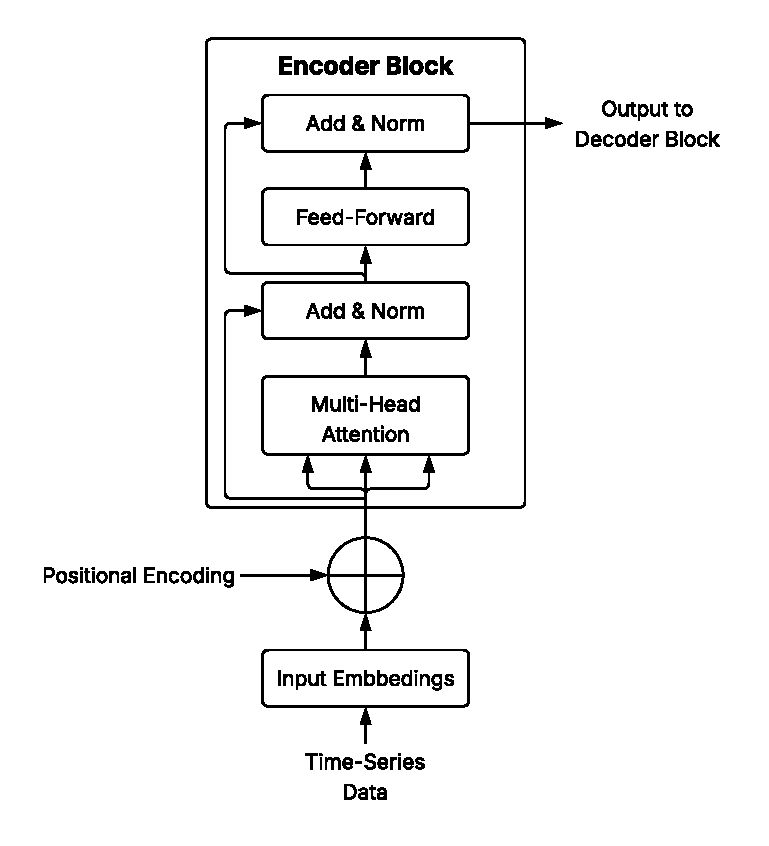
\includegraphics[width=0.7\textwidth]{figures/Transformer_Encoder.pdf}
     \caption{Diagrama esquemático de un bloque codificador (\textit{Encoder Block}) de Transformer aplicado a series temporales.}
     \label{fig:transformer_encoder}
 \end{figure}

Las capas de atención en los Transformers capturan dependencias de largo alcance e interacciones entre los elementos dentro de la ventana de observación. Cuando se combinan con arquitecturas recurrentes, modelan conjuntamente la estructura global y secuencial. Avances recientes incluyen mecanismos de atención jerárquicos y a múltiples escalas, así como adaptaciones que mejoran la eficiencia para secuencias largas y conjuntos de datos pequeños~\cite{wen2023survey}.

\section{Detección de fallos basada en error de modelo}

\section{Calidad del dato y normas internacionales (ISO 15197)}

\section {Estado del arte: trabajos relacionados} % (del protocolo, sec. II — Antecedentes)

\section{Trabajo previo del grupo de investigación} %  (referencia explícita al paper Algorithms 2025 como punto de partida)

% =================================================
% CAPÍTULO 3. METODOLOGÍA
% =================================================
\chapter{Metodología}

\section{Visión general del sistema} % (diagrama de la "Metodología Actual")


\section{Conjuntos de datos} %(del paper, sec. 2.1)
\label{sec:datasets}
La validación de un sistema de detección de fallos e imputación en línea para CGM requiere disponer de fuentes de datos con propiedades complementarias. Por un lado, se necesita un entorno en el que se conozca con exactitud el valor verdadero de la glucosa y la naturaleza de los fallos presentes en la señal, condición indispensable para cuantificar el error de imputación y la exactitud de la detección mediante métricas objetivas. Por otro lado, se requieren registros clínicos reales que reflejen la variabilidad fisiológica de pacientes con diabetes tipo 1 y los modos de fallo característicos del uso ambulatorio de los dispositivos comerciales de CGM, condición indispensable para evaluar la generalización del sistema fuera del entorno de entrenamiento.

En consecuencia, este trabajo emplea dos fuentes de datos complementarias. La primera consiste en datos sintéticos generados a partir del modelo fisiológico multicompartimental de Sorensen~\cite{ruiz2018sorensen}, los cuales se utilizan tanto para el entrenamiento de las arquitecturas profundas como para una evaluación cuantitativa controlada con fallos inyectados de manera artificial sobre un conjunto de prueba independiente. La segunda corresponde al conjunto clínico OhioT1DM~\cite{marling2020ohiot1dm}, que reúne registros reales de pacientes con diabetes tipo 1 y se emplea para validar el comportamiento del sistema bajo las condiciones no controladas del uso clínico cotidiano. Esta estrategia bifásica permite combinar el rigor cuantitativo, posible únicamente cuando se dispone de una señal de referencia, con la evidencia de generalización a datos reales, donde no es posible cuantificar el error de reconstrucción pero sí evaluar el comportamiento del detector y de la imputación de manera cualitativa y mediante métricas de clasificación.

\subsection{Datos sintéticos: modelo fisiológico de Sorensen}
\label{subsec:datos_sinteticos}
Para reproducir la dinámica glucosa--insulina--carbohidratos en un adulto con diabetes mellitus tipo 1 (DT1) se utilizó el modelo fisiológico compartimental de Sorensen~\cite{ruiz2018sorensen}. Este modelo está conformado por 19 ecuaciones diferenciales ordinarias (EDO) que representan los flujos de glucosa, insulina, glucagón y otros procesos metabólicos a través de los principales compartimentos del organismo --hígado, riñón, tejidos periféricos y región subcutánea--, capturando las interacciones fisiológicas no lineales descritas en el Apéndice~\ref{app:sorensen}.

La simulación contempla absorción continua tanto para la insulina como para los carbohidratos, en lugar de impulsos instantáneos, reflejando así la dinámica biológica realista del organismo. La concentración de glucosa $G_{CGM}(t)$ representa la glucosa plasmática medida por un sensor CGM (mg/dL); la concentración de insulina $I(t)$ denota la insulina plasmática tras la administración basal y de bolos (mU/L); y la ingesta de carbohidratos $\mathit{CHO}(t)$ modela las tasas de absorción gastrointestinal (mg/min).

Se generaron 1\,400 observaciones muestreadas cada 5~min sobre un horizonte simulado de 5~días, proporcionando una granularidad temporal suficiente para capturar la variabilidad de la glucosa, la dinámica de la insulina y la absorción de los alimentos, como se ilustra en la Figura~\ref{fig:datos_sinteticos}. Al incorporar retardos fisiológicos de absorción y respuestas metabólicas no lineales, el modelo de Sorensen produce datos realistas y libres de artefactos, lo que constituye un entorno virtual confiable para evaluar estrategias de detección de fallos, algoritmos de control y métodos de imputación en línea bajo condiciones cercanas a las clínicas. Este conjunto se emplea para el entrenamiento y la validación interna de las redes neuronales. Adicionalmente, una segunda simulación independiente del modelo, descrita en la Sección~\ref{subsec:inyeccion_fallos}, se utiliza como conjunto de prueba con fallos inyectados de manera controlada para la evaluación cuantitativa final del sistema.

 \begin{figure}[h]
     \centering
     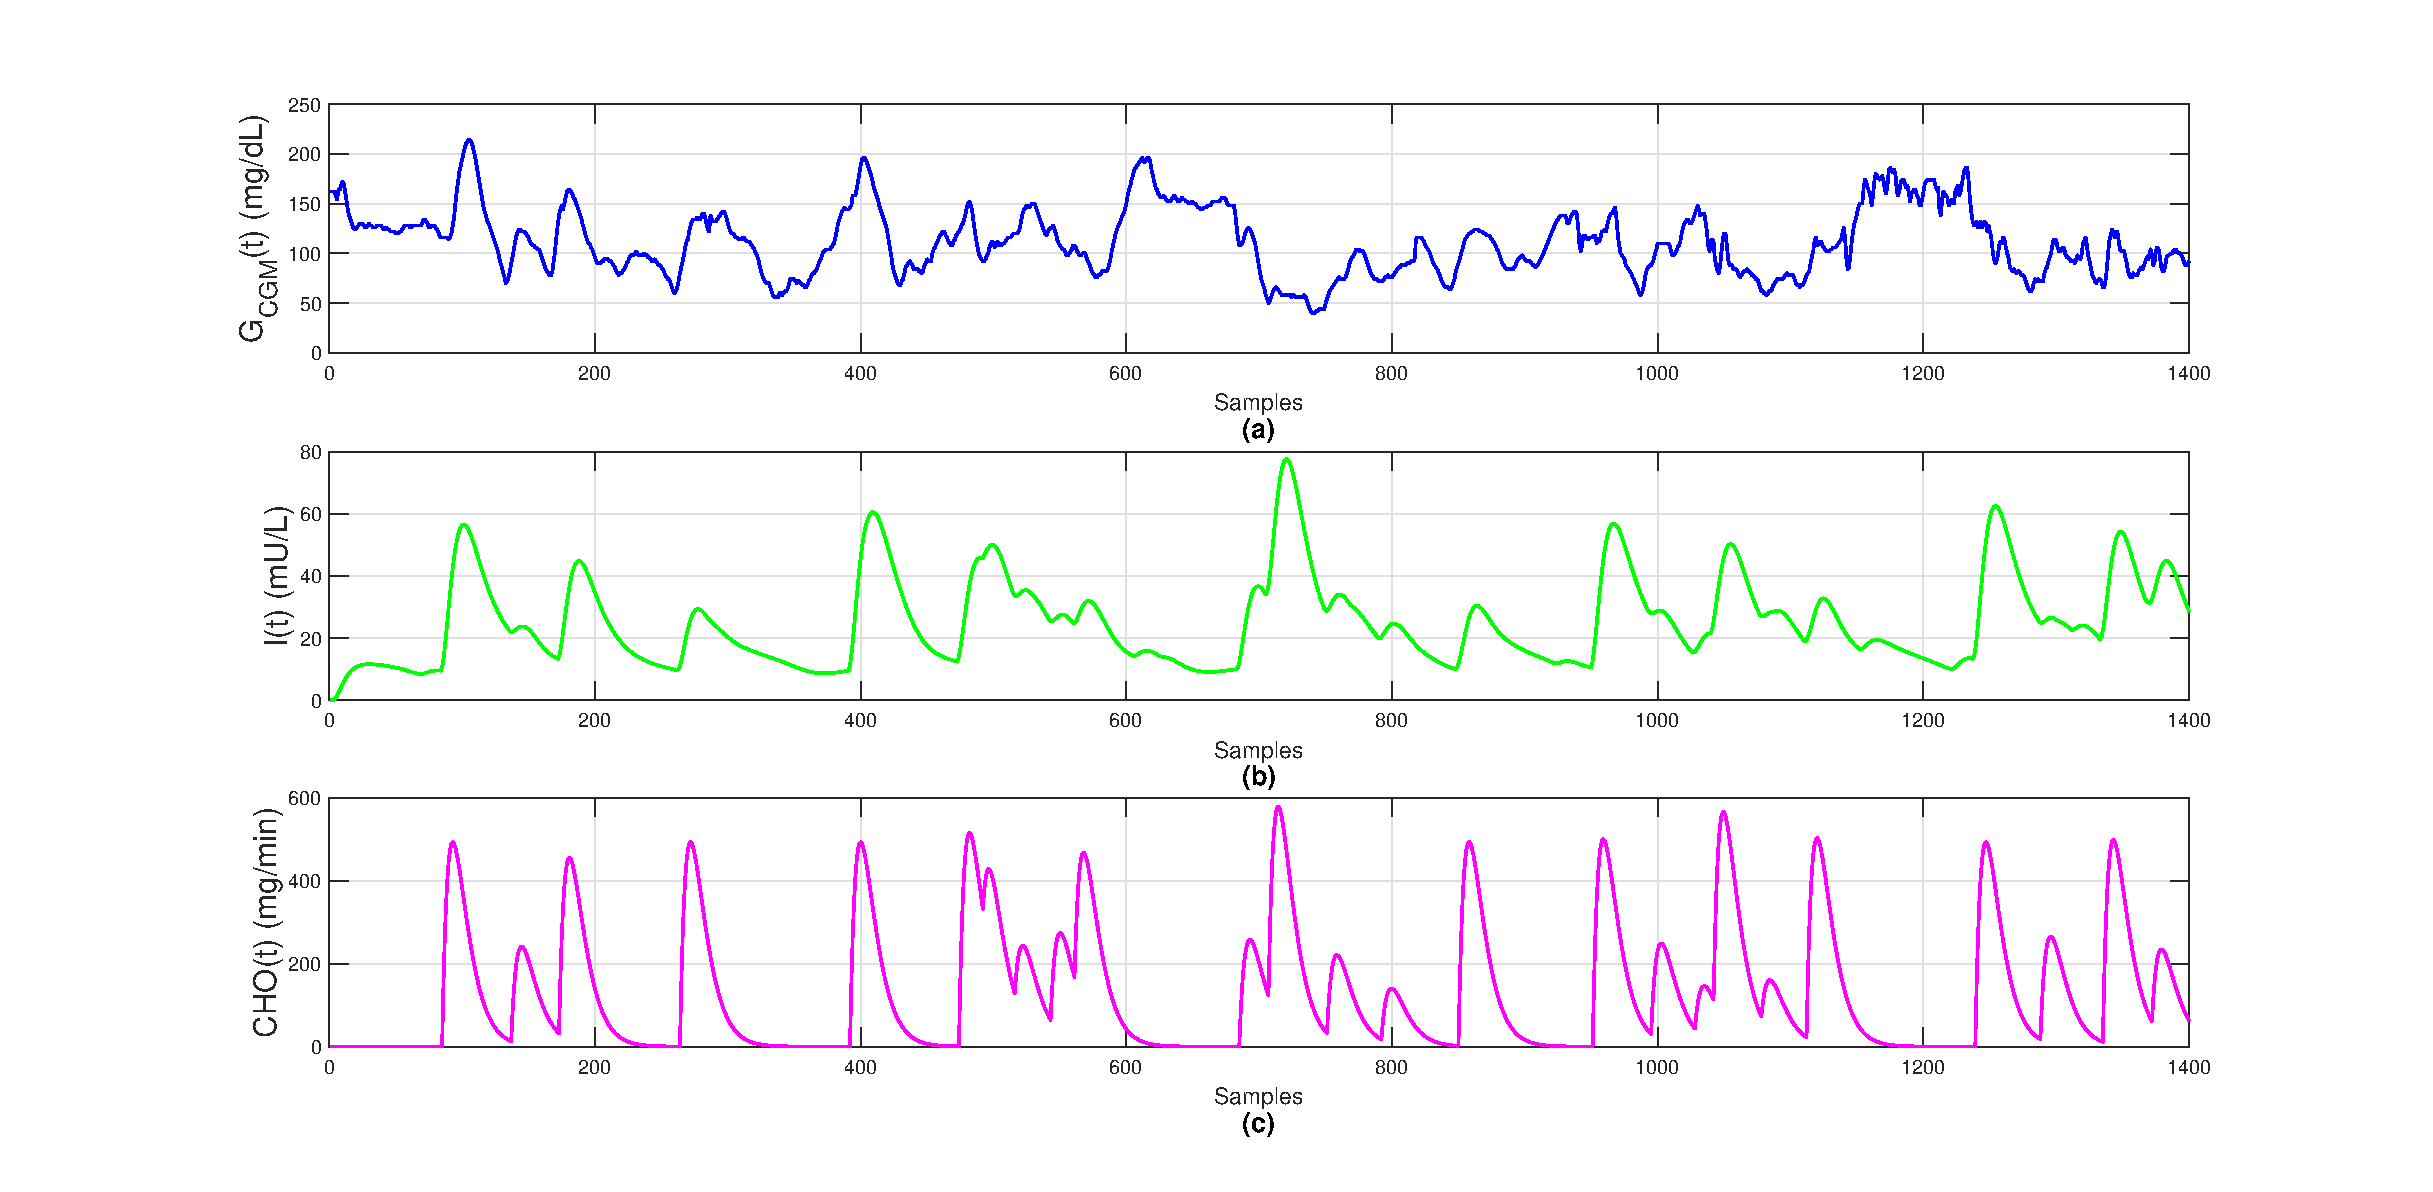
\includegraphics[width=0.9\textwidth]{figures/Datos_sinteticos.eps}
     \caption{Datos simulados con el modelo de Sorensen: (a) glucosa en sangre $G_{CGM}(t)$; (b) insulina plasmática $I(t)$; (c) absorción de carbohidratos $\mathit{CHO}(t)$.}
     \label{fig:datos_sinteticos}
 \end{figure}
\subsubsection*{Variables fisiológicas de entrada}

La insulina exógena reduce la glucosa plasmática con un efecto retardado determinado por la cinética de absorción y eliminación subcutánea, mientras que las comidas afectan la glicemia mediante la digestión de carbohidratos y su absorción intestinal. Por lo tanto, incluir la dosis de insulina y la ingesta de carbohidratos como entradas del modelo es fisiológicamente apropiado, y expresarlas como perfiles de absorción alinea las entradas con su temporalidad causal, simplificando el aprendizaje en los modelos recurrentes y mejorando la precisión predictiva~\cite{munoz2021learning}.

En consecuencia, el vector de entrada del sistema propuesto incluye señales de insulina y carbohidratos como variables exógenas que rigen la glicemia y las estructura de manera que reflejen las respuestas fisiológicas retardadas. Esta representación permite que los modelos profundos aprendan la temporalidad real de la dinámica posprandial~\cite{munoz2021learning}. Más allá del total de carbohidratos, la composición de las comidas también influye en las fases tardías de la excursión glucémica, mejorando las predicciones a horizontes de 30 a 60~min y favoreciendo el modelado específico por sujeto~\cite{annuzzi2023impact}.

\subsection{Datos clínicos reales: OhioT1DM}
\label{subsec:datos_reales}

El conjunto OhioT1DM contiene ocho semanas de registros para cada uno de doce pacientes con diabetes mellitus tipo 1, aportados de manera anónima e identificados únicamente por un número aleatorio. Todos los participantes utilizaban terapia con bomba de insulina y monitoreo continuo de glucosa, equipados con bombas Medtronic 530G o 630G y sensores Medtronic Enlite. La cohorte se distribuye en dos grupos liberados en años distintos: el primero, conformado por seis pacientes que utilizaban la pulsera de actividad Basis Peak, fue publicado en 2018 con motivo del primer \textit{Blood Glucose Level Prediction Challenge}; el segundo, conformado por seis pacientes que utilizaban la pulsera Empatica Embrace, se incorporó en 2020 para la segunda edición de dicho reto. La Tabla~\ref{tab:ohio_cohort} resume las características demográficas y de instrumentación de los doce pacientes.

\begin{table}[H]
    \centering
    \caption{Composición de la cohorte del conjunto OhioT1DM~\cite{marling2020ohiot1dm}.}
    \label{tab:ohio_cohort}
    \begin{tabular}{ccccc}
        \toprule
        \textbf{ID} & \textbf{Sexo} & \textbf{Rango de edad} & \textbf{Bomba} & \textbf{Pulsera (cohorte)} \\
        \midrule
        540 & Masculino & 20--40 & 630G & Empatica (2020) \\
        544 & Masculino & 40--60 & 530G & Empatica (2020) \\
        552 & Masculino & 20--40 & 630G & Empatica (2020) \\
        567 & Femenino  & 20--40 & 630G & Empatica (2020) \\
        584 & Masculino & 40--60 & 530G & Empatica (2020) \\
        596 & Masculino & 60--80 & 530G & Empatica (2020) \\
        559 & Femenino  & 40--60 & 530G & Basis (2018) \\
        563 & Masculino & 40--60 & 530G & Basis (2018) \\
        570 & Masculino & 40--60 & 530G & Basis (2018) \\
        575 & Femenino  & 40--60 & 530G & Basis (2018) \\
        588 & Femenino  & 40--60 & 530G & Basis (2018) \\
        591 & Femenino  & 40--60 & 530G & Basis (2018) \\
        \bottomrule
    \end{tabular}
\end{table}

Cada paciente cuenta con un volumen de aproximadamente entre 9\,000 y 12\,600 muestras de entrenamiento y entre 2\,300 y 2\,900 muestras de prueba, distribuidas en dos archivos XML por sujeto.

\subsubsection*{Variables registradas}

El conjunto OhioT1DM integra de manera sincronizada múltiples flujos de información asociados al paciente. Las variables principales utilizadas en este trabajo son: la glucosa medida por el sensor CGM con una cadencia de 5~min, las dosis de insulina administradas (basal continua, basal temporal y bolos), y los registros auto-reportados de comidas con su correspondiente estimación de carbohidratos. De manera complementaria, el conjunto incluye otras variables que pueden enriquecer el análisis fisiológico: glucemias capilares de auto-monitoreo (\textit{finger sticks}), reportes de sueño con calificación subjetiva de calidad, periodos de trabajo, episodios de estrés, hipoglucemia sintomática, enfermedad y ejercicio, así como datos provenientes de la pulsera de actividad (frecuencia cardiaca, respuesta galvánica de la piel, temperatura cutánea, conteo de pasos, detección de sueño y magnitud de aceleración, según el modelo de pulsera).

\subsubsection*{Disponibilidad y proceso de obtención}

El conjunto OhioT1DM se distribuye públicamente con fines exclusivamente de investigación a través de un \textit{Data Use Agreement} (DUA) firmado entre la institución del investigador y Ohio University. Los datos fueron desidentificados conforme al método \textit{Safe Harbor} establecido por la regulación HIPAA, y todas las fechas de cada paciente fueron desplazadas de manera uniforme hacia el futuro para preservar los días de la semana y los horarios de cada evento, sin que sea posible inferir efectos estacionales o festividades. Para el desarrollo de esta tesis se siguió el procedimiento formal correspondiente con la Universidad de Guadalajara para obtener el conjunto.

\subsubsection*{Uso del conjunto en este trabajo}

A diferencia de los datos sintéticos, las series del conjunto OhioT1DM contienen fallos de sensor no controlados que se manifiestan como ruido y datos faltantes derivados de desconexiones naturales del dispositivo durante el uso ambulatorio. La Tabla~\ref{tab:ohio_gaps} muestra los cinco intervalos más largos con datos faltantes identificados en el sujeto evaluado en el trabajo previo del grupo, los cuales pueden alcanzar hasta más de 16~h de duración. Cabe señalar que, aunque la presencia de ruido también es esperable en estos registros, no es posible corroborarla directamente, ya que el conjunto no incluye una señal de glucosa de referencia que permita comparar las lecturas del sensor con un valor verdadero.

\begin{table}[H]
    \centering
    \caption{Cinco intervalos más largos con datos faltantes identificados en el sujeto evaluado del conjunto OhioT1DM.}
    \label{tab:ohio_gaps}
    \begin{tabular}{lcc}
        \toprule
        \textbf{Inicio} & \textbf{Fin} & \textbf{Duración (h)} \\
        \midrule
        2021-12-07 00:00 & 2021-12-07 16:20 & 16.4 \\
        2022-01-07 18:30 & 2022-01-08 06:25 & 12.0 \\
        2022-01-09 01:20 & 2022-01-09 06:10 & 4.9 \\
        2021-12-24 02:55 & 2021-12-24 07:00 & 4.2 \\
        2021-12-18 05:00 & 2021-12-18 08:30 & 3.6 \\
        \bottomrule
    \end{tabular}
\end{table}

La ausencia de una traza de glucosa de referencia implica que sobre OhioT1DM solo es posible reportar métricas de clasificación para la detección de fallos, complementadas con un análisis cualitativo del comportamiento de la imputación durante los segmentos faltantes. Esta limitación motiva el uso complementario del conjunto sintético basado en Sorensen, que sí dispone de una señal de referencia y, por lo tanto, permite cuantificar el error de reconstrucción mediante métricas de regresión.

En el trabajo previo del grupo de investigación~\cite{sanchez2025imputation} la validación clínica se realizó sobre un único paciente del conjunto OhioT1DM. En la presente tesis se contempla extender esta validación a un subconjunto de entre tres y cinco pacientes con el objetivo de evaluar la variabilidad inter-sujeto y la capacidad de generalización del sistema bajo condiciones reales heterogéneas, sin requerir un nuevo entrenamiento de los modelos.

\subsection{Inyección controlada de fallos}
\label{subsec:inyeccion_fallos}

Para evaluar la capacidad del sistema de detectar datos anómalos o faltantes y de realizar la imputación en línea, se generó un conjunto de prueba independiente a partir de una nueva simulación del modelo de Sorensen, el cual no se utilizó durante el entrenamiento ni durante el ajuste de hiperparámetros, garantizando así una evaluación imparcial del desempeño final. Este conjunto consta de 1\,400 muestras sintéticas de glucosa generadas bajo condiciones realistas que incluyen variaciones en los patrones de comidas y dosis de insulina, emulando escenarios típicos en personas con DT1.

Posteriormente, se introdujo corrupción en los datos mediante la inyección controlada de anomalías y segmentos faltantes, reproduciendo dos modos de fallo comúnmente observados en sensores CGM~\cite{sanchez2023realtime}:

\begin{itemize}
    \item \textbf{(F1) Ráfagas de ruido blanco:} estos fallos se manifiestan como fluctuaciones bruscas y de corta duración en la señal de glucosa, originadas por ruido electrónico o térmico, degradación del sensor, problemas de cableado, interferencia electromagnética o desplazamientos leves en la interfaz sensor--tejido. Para reproducir este efecto se añadió ruido gaussiano con desviación estándar $\sigma = 5.6$~mg/dL y amplitud máxima de 30~mg/dL en segmentos aleatorios de 20 a 40 muestras.
    
    \item \textbf{(F2) Desconexiones del sensor:} estos fallos se presentan como caídas súbitas de la señal a valores cercanos a cero o indefinidos (NaN), típicamente como consecuencia de problemas severos de hardware tales como pérdida de alimentación, desconexión parcial o total, o interrupción del contacto con el tejido subcutáneo. Para modelar este escenario, las lecturas de glucosa fueron reemplazadas por valores cercanos a cero en dos segmentos de 50 y 20 muestras, correspondientes aproximadamente a 4~h y 1.5~h, respectivamente. Este evento se categoriza como un error de desconexión o dato faltante.
\end{itemize}

Las amplitudes de ruido ($\sigma = 5.6$~mg/dL) y las duraciones de las desconexiones (1.5~h y 4~h) representan perturbaciones típicas en dispositivos CGM comerciales. Análisis de exactitud reportados para el dispositivo FreeStyle Libre Pro indican desviaciones medias del orden de $\pm 15$~mg/dL y pérdidas transitorias de señal de hasta varias horas en entornos clínicos~\cite{huang2022accuracy}, lo cual es consistente con las magnitudes adoptadas en este estudio.

La introducción de estos fallos en el conjunto de prueba genera condiciones realistas para evaluar la robustez y la exactitud de los métodos de detección de fallos e imputación propuestos. La Figura~\ref{fig:test_corrupto} muestra la traza de glucosa sintética del conjunto de prueba, junto con las regiones afectadas por cada uno de los dos tipos de fallo inyectados.

 \begin{figure}[h]
     \centering
     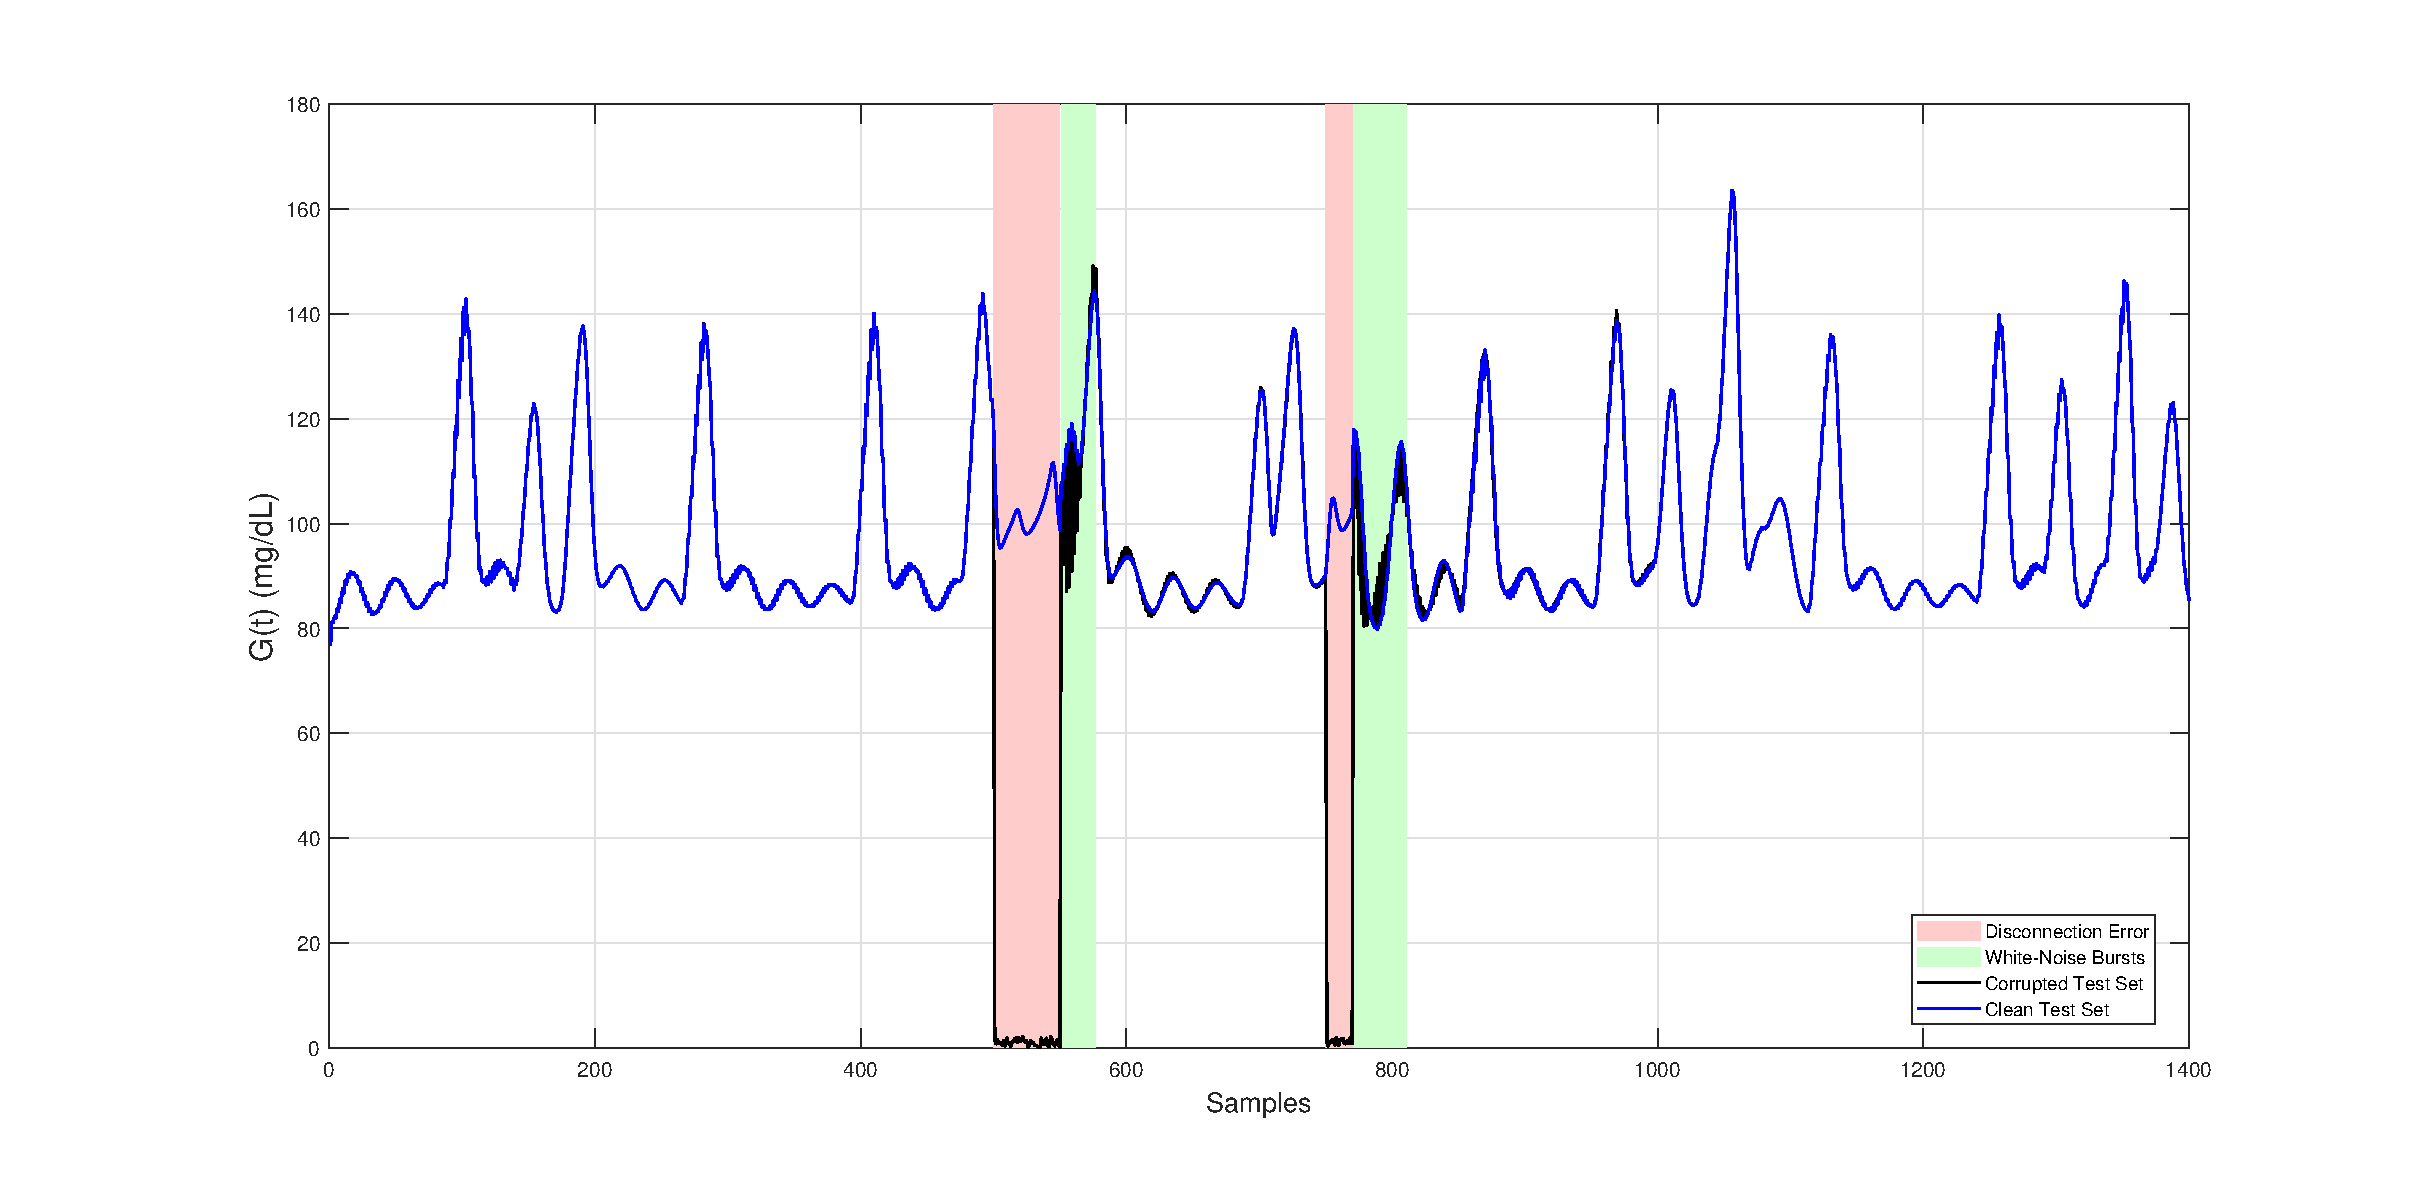
\includegraphics[width=0.9\textwidth]{figures/Test_corrupto.eps}
     \caption{Traza de glucosa CGM simulada utilizada como conjunto de prueba independiente. La señal limpia (azul) representa los niveles fisiológicamente realistas de glucosa generados por el modelo de Sorensen. La señal corrupta (negro) incluye los dos tipos de fallo inyectados: ráfagas de ruido blanco (regiones sombreadas en verde) y desconexiones del sensor (regiones sombreadas en rojo).}
     \label{fig:test_corrupto}
 \end{figure}

\section{Preprocesamiento y ventana deslizante}
\label{sec:preprocesamiento}

Antes de alimentar las arquitecturas neuronales descritas en la Sección~\ref{sec:redes_neuronales_profundas}, las series temporales descritas en la Sección~\ref{sec:datasets} requieren ser organizadas en un formato compatible con la operación punto a punto del sistema. Este preprocesamiento involucra cuatro pasos consecutivos: la partición cronológica del conjunto de datos, una limpieza mínima de la señal, la normalización de las variables de entrada para homogeneizar sus escalas, y la construcción de una representación basada en ventana deslizante que codifica las dependencias temporales en cada vector de entrada. Cada uno de estos pasos se describe a continuación.

\subsection{Partición cronológica del conjunto de datos}
\label{subsec:particion_datos}

El conjunto sintético de Sorensen utilizado para el entrenamiento y la validación interna se dividió de forma cronológica en una proporción 80/20: el primer 80\,\% de las muestras (1\,120 observaciones) se destinó al entrenamiento y el 20\,\% restante (280 observaciones) a la validación interna. Esta partición se realizó de manera determinista, fijando una semilla aleatoria, con el fin de garantizar la reproducibilidad de los experimentos.

A diferencia de las particiones aleatorias empleadas habitualmente en problemas de clasificación o regresión sobre datos i.i.d., una partición cronológica resulta indispensable cuando se trabaja con series temporales. Una división aleatoria permitiría que muestras del futuro se filtraran al conjunto de entrenamiento, generando una fuga de información (\textit{data leakage}) que sobreestima artificialmente el desempeño del modelo y compromete la validez de la evaluación~\cite{scholz2004metabolite}. Al respetar el orden temporal, la partición cronológica preserva la estructura secuencial de las señales fisiológicas y emula la condición real bajo la cual el modelo deberá operar: predecir muestras futuras a partir únicamente de información pasada.

La validación final del sistema se realiza sobre el conjunto de prueba independiente con fallos inyectados, descrito en la Sección~\ref{subsec:inyeccion_fallos}, así como sobre los registros reales del conjunto OhioT1DM (Sección~\ref{subsec:datos_reales}). Ninguno de estos conjuntos participa en el entrenamiento ni en el ajuste de hiperparámetros.

\subsection{Limpieza mínima de la señal}
\label{subsec:limpieza}

Dado que la detección de fallos y la imputación se realizan en línea, el preprocesamiento aplicado a la señal de glucosa se mantiene deliberadamente mínimo. No se aplica eliminación de valores atípicos ni suavizado, ya que un filtrado agresivo podría eliminar variaciones informativas que son precisamente las que el sistema debe aprender a reconocer como genuinas o anómalas en tiempo real~\cite{scholz2004metabolite}.

La única corrección aplicada consiste en reemplazar valores de glucosa inferiores a 10~mg/dL, considerados fisiológicamente inviables y atribuibles a fallos severos del sensor, por la última predicción válida del modelo. Esta sustitución previene inestabilidades numéricas durante el entrenamiento sin alterar la dinámica fisiológica subyacente. El resto de la señal, incluidas las fluctuaciones rápidas y las variaciones inducidas por la dinámica posprandial, se conserva íntegramente para que las redes neuronales puedan aprender los patrones característicos del comportamiento glucémico.

\subsection{Normalización de las variables de entrada}
\label{subsec:normalizacion}

Las tres variables que conforman el vector de entrada del modelo --glucosa, insulina y carbohidratos-- presentan escalas y unidades heterogéneas: la glucosa se expresa en mg/dL y suele oscilar entre 70 y 250~mg/dL, la insulina plasmática se mide en mU/L con valores típicos entre 0 y 80~mU/L, y la absorción de carbohidratos se reporta en mg/min con valores que pueden alcanzar los 600~mg/min durante las excursiones posprandiales. Esta disparidad de escalas, si se introdujera directamente en una red neuronal, llevaría a que las variables con magnitudes mayores dominaran las actualizaciones del gradiente, dificultando la convergencia y sesgando la representación aprendida.

Para evitar este efecto se aplicó una normalización z-score independiente para cada variable, definida como:

\begin{equation}
\label{eq:zscore}
\tilde{v}(k) = \frac{v(k) - \mu_v}{\sigma_v},
\end{equation}

donde $v(k) \in \{g(k), u(k), m(k)\}$ representa el valor original de la variable en el instante $k$, $\tilde{v}(k)$ su valor normalizado, y $\mu_v$ y $\sigma_v$ corresponden a la media y la desviación estándar calculadas exclusivamente sobre el subconjunto de entrenamiento. Estos parámetros estadísticos se almacenan tras la fase de entrenamiento y se reutilizan idénticos durante la operación en línea, garantizando que cualquier nueva muestra se transforme en el mismo espacio sobre el cual fue entrenada la red. Este procedimiento es el estándar para evitar fugas de información estadística desde los conjuntos de validación o prueba.

Tras la predicción, la salida normalizada de la red se reescala al rango original mediante la operación inversa $\hat{g}(k) = \tilde{\hat{g}}(k) \cdot \sigma_g + \mu_g$, recuperando así una estimación de glucosa expresada en mg/dL e interpretable clínicamente.

\subsection{Construcción de la ventana deslizante}
\label{subsec:ventana_deslizante}

Las redes neuronales empleadas en este trabajo utilizan conjuntamente las señales de glucosa, insulina y carbohidratos como entradas para la predicción y la imputación. Las dependencias temporales se capturan mediante un esquema de ventana deslizante que genera un vector de entrada en cada paso de tiempo discreto. Cada vector, o ventana, está conformado por ocho elementos: las seis lecturas más recientes de glucosa, el valor actual de insulina y la ingesta actual de carbohidratos, proporcionando una representación compacta pero informativa de la fisiología reciente.

Formalmente, en cada paso de tiempo $k$ el vector de entrada $\mathbf{x}(k)$ se define como:

\begin{equation}
\label{eq:ventana}
\mathbf{x}(k) = \big[\, g(k\!-\!6),\ g(k\!-\!5),\ g(k\!-\!4),\ g(k\!-\!3),\ g(k\!-\!2),\ g(k\!-\!1),\ u(k),\ m(k)\,\big]^{T},
\end{equation}

donde $g(k\!-\!i)$ representa la medición de glucosa en el instante $k\!-\!i$ (mg/dL), $u(k)$ es la concentración de insulina (mU/L) y $m(k)$ denota la ingesta de carbohidratos (mg/min).

La elección de un horizonte histórico de $d = 6$ pasos no es arbitraria: a una cadencia de muestreo de 5~min, esto corresponde a 30~min de historia reciente de glucosa, intervalo que coincide con la escala temporal típica de las excursiones glucémicas posprandiales y con la respuesta de la insulina exógena de acción rápida. Una ventana sustancialmente menor no capturaría tendencias suficientemente informativas, mientras que una ventana mucho mayor introduciría redundancia y aumentaría el costo computacional sin un beneficio predictivo proporcional. La inclusión de la insulina y los carbohidratos como valores instantáneos --y no como historial-- responde a que estas variables ya están expresadas como perfiles de absorción continuos (Sección~\ref{subsec:datos_sinteticos}) y, por lo tanto, su valor actual incorpora implícitamente la dinámica retardada de su efecto fisiológico.

Aunque las redes neuronales \textit{feedforward} no son intrínsecamente temporales, la formulación basada en ventana deslizante codifica las dependencias temporales directamente en el vector de entrada. De manera general, el mapeo aprendido por cualquiera de las arquitecturas puede expresarse como una función no lineal de la forma:

\begin{equation}
\label{eq:mapeo_general}
\hat{g}(k) = f_{\Theta}\big(\,\mathbf{x}_W(k),\ \mathbf{s}(k-1)\,\big),
\end{equation}

donde

\begin{equation}
\label{eq:ventana_general}
\mathbf{x}_W(k) = \big[\, g(k-d),\ \ldots,\ g(k-1),\ u(k),\ m(k)\,\big]^{T}
\end{equation}

agrupa las últimas $d$ lecturas de glucosa junto con las entradas actuales de insulina y carbohidratos. Esta estructura asegura que tanto la dinámica endógena (historia de la glucosa) como los reguladores fisiológicos exógenos (absorción de insulina y de los alimentos) sean capturados.

La función $f_{\Theta}(\cdot)$, parametrizada por los pesos $\Theta$, representa el mapeo general común a todas las arquitecturas. Los modelos recurrentes (LSTM, GRU) mantienen un estado oculto $\mathbf{s}(k)$ para modelar dependencias de largo plazo; los modelos convolucionales (1D-CNN) infieren correlaciones temporales locales mediante \textit{kernels}; y los modelos basados en atención (Transformer-LSTM) ponderan todos los elementos de la entrada para capturar interacciones globales.

\subsection{Operación deslizante en línea}
\label{subsec:operacion_online}

Durante la fase de entrenamiento, la ventana se desplaza con un paso (\textit{stride}) igual a 1, generando un nuevo par entrada--salida en cada instante de tiempo y asegurando la alineación temporal entre las tendencias de glucosa y los reguladores fisiológicos. Esta configuración garantiza la disponibilidad de un volumen suficiente de pares para el aprendizaje y permite que el modelo aprenda una predicción punto a punto.

Durante la operación en línea, la ventana se actualiza de manera deslizante con cada nueva muestra recibida del sensor: el vector $\mathbf{x}(k)$ se construye descartando la lectura de glucosa más antigua y agregando la más reciente, manteniendo siempre las últimas $d$ lecturas como contexto histórico. Cuando un valor de glucosa dentro de la ventana es identificado como faltante o ha sido marcado como fallo por el detector descrito en la Sección~\ref{sec:deteccion_fallos}, dicho valor se reemplaza por la última predicción válida del modelo antes de incorporar la ventana al siguiente paso de inferencia. Este mecanismo preserva la continuidad de la entrada durante la operación en línea y evita la propagación de fallos a las predicciones subsecuentes.

% \begin{figure}[h]
%     \centering
%     \includegraphics[width=0.85\textwidth]{figures/ventana_deslizante.png}
%     \caption{Esquema de la ventana deslizante de entrada al modelo. En cada paso $k$ se concatenan las seis lecturas más recientes de glucosa con los valores actuales de insulina y absorción de carbohidratos para formar el vector $\mathbf{x}(k)$ de ocho componentes. Durante la operación en línea, los valores marcados como fallo son reemplazados por la predicción del modelo antes de incorporarse a la siguiente ventana.}
%     \label{fig:ventana_deslizante}
% \end{figure}

Esta estructura permite la detección y la imputación punto a punto de los niveles de glucosa en tiempo real, manteniendo la robustez ante fallos del sensor o vacíos de información. La Sección~\ref{sec:arquitecturas_implementadas} describe en detalle las cuatro arquitecturas neuronales implementadas que operan sobre este esquema.

\section{Arquitecturas implementadas} % (del paper, sec. 4.1)
\label{sec:arquitecturas_implementadas}

Sobre el esquema común de preprocesamiento y ventana deslizante descrito en la Sección~\ref{sec:preprocesamiento}, este trabajo implementa cuatro arquitecturas de redes neuronales profundas con paradigmas de procesamiento complementarios: una arquitectura recurrente eficiente (GRU), una arquitectura puramente convolucional (1D-CNN), una arquitectura híbrida que combina convolución y recurrencia (CNN--LSTM) y una arquitectura híbrida que combina atención y recurrencia (Transformer--LSTM). Esta selección no es arbitraria: cada paradigma capta de manera distinta las dependencias temporales en la señal de glucosa, y comparar los cuatro permite evaluar qué tipo de inductive bias resulta más adecuado para la detección de fallos y la imputación en línea de datos de CGM.

Adicionalmente, se incluyen dos modelos de comparación que sirven como referencia: un modelo estadístico clásico (ARIMA) que actúa como línea base lineal y un modelo convolucional causal de uso establecido en series temporales (TCN). Estos modelos no forman parte de las arquitecturas propuestas, pero permiten contextualizar el desempeño de los modelos profundos frente a alternativas tradicionales.

A lo largo de esta sección, todas las arquitecturas reciben como entrada el vector $\mathbf{x}(k) \in \mathbb{R}^{8}$ definido en la Ecuación~\eqref{eq:ventana} y producen como salida la predicción escalar $\hat{g}(k)$ correspondiente al siguiente paso de glucosa. Las configuraciones específicas de cada arquitectura --número de unidades, filtros, tasas de \textit{dropout}-- corresponden a las empleadas en el trabajo previo del grupo de investigación~\cite{sanchez2025imputation} y se mantienen idénticas en esta tesis para garantizar que las extensiones propuestas (Capítulos~\ref{subsec:umbral_adaptativo} y~\ref{sec:pipeline_desacoplado}) se evalúen sobre una base arquitectónica comparable.


\subsection{Red Híbrida CNN-LSTM}
\label{subsec:arq_cnn_lstm}

La arquitectura CNN--LSTM combina ambos paradigmas en una topología secuencial. Una primera capa convolucional unidimensional de 16 filtros y \textit{kernel} 3, seguida por activación ReLU, opera como extractor de características locales sobre el vector de entrada. Las características extraídas son procesadas por una capa LSTM de 32 unidades, cuya salida pasa por una capa de \textit{dropout} del 30\,\%, una capa densa de 64 unidades con activación ReLU, y finalmente una capa densa de salida con una unidad lineal.

La motivación de esta arquitectura es complementar las fortalezas de ambos paradigmas: la capa convolucional extrae patrones locales --por ejemplo, transiciones bruscas entre muestras adyacentes que pueden indicar ruido-- y la capa recurrente LSTM, descrita por las Ecuaciones~\eqref{eq:lstm} de la Sección~\ref{subsec:lstm}, integra esos patrones a lo largo del tiempo, modelando dependencias de plazo más extenso como los efectos retardados de la insulina y la digestión de los carbohidratos. Esta combinación es la que mejor desempeño presentó en el trabajo previo en términos de detección de fallos.


\subsection{GRU}
\label{subsec:arq_gru}

La arquitectura GRU constituye la opción recurrente más eficiente en términos de número de parámetros. Está conformada por una única capa GRU de 32 unidades que procesa secuencialmente el vector de entrada, seguida por una capa de \textit{dropout} con tasa del 30\,\% que mitiga el sobreajuste, una capa densa de 64 unidades con activación ReLU que actúa como bloque de proyección, y una capa densa final con una sola unidad y función de activación lineal que produce la predicción de glucosa $\hat{g}(k)$.

El estado oculto de la celda GRU, descrito por las Ecuaciones~\eqref{eq:gru} de la Sección~\ref{subsec:gru}, encapsula las dependencias temporales acumuladas a lo largo de la secuencia, mientras que el bloque denso final transforma esa representación oculta en una predicción puntual. Al usar un mecanismo de compuertas más compacto que el de LSTM, esta arquitectura ofrece una latencia de inferencia reducida, característica deseable para la operación en línea sobre dispositivos con recursos limitados.


\subsection{1D-CNN}
\label{subsec:arq_1dcnn}

La arquitectura 1D-CNN es puramente convolucional, sin componentes recurrentes ni de atención. La señal de entrada atraviesa dos bloques convolucionales sucesivos: el primero aplica una convolución unidimensional con 32 filtros de \textit{kernel} 5 seguida por activación ReLU, una capa de \textit{dropout} del 20\,\% y una operación de \textit{max-pooling}; el segundo bloque aplica una convolución con 32 filtros de \textit{kernel} 3, seguida nuevamente por ReLU. Posteriormente, una capa de \textit{Global Average Pooling} resume los mapas de características en un vector de tamaño fijo, que es procesado por una capa densa de 64 unidades con activación ReLU y, finalmente, por una capa densa de salida con una unidad lineal.

Esta arquitectura está diseñada para extraer patrones temporales locales sin mantener un estado interno entre pasos de tiempo, lo que la hace particularmente adecuada para identificar la firma característica de las ráfagas de ruido de alta frecuencia descritas en el escenario de fallo F1 (Sección~\ref{subsec:inyeccion_fallos}). El uso de \textit{Global Average Pooling} en lugar de un \textit{flatten} reduce drásticamente el número de parámetros y favorece la generalización, evitando que la red memorice posiciones absolutas dentro de la ventana de entrada.

\subsection{Red Híbrida Transformer-LSTM}
\label{subsec:arq_transformer_lstm}

La arquitectura Transformer--LSTM es la más compleja de las cuatro. Inicia con una capa de \textit{embedding} de 32 dimensiones que proyecta el vector de entrada a un espacio de mayor dimensionalidad, sumándole una codificación posicional para preservar la información de orden temporal. La señal proyectada atraviesa luego dos bloques de atención multi-cabeza con cuatro cabezas de 32 canales cada una, cada bloque acompañado por una conexión residual y una normalización por capa (\textit{LayerNorm}). Posteriormente, la representación obtenida se procesa por dos capas LSTM consecutivas de 32 unidades, intercaladas con \textit{dropout} del 30\,\%, y finalmente una capa densa con una unidad lineal genera la predicción.

Tal como se describe en la Sección~\ref{subsec:transformer}, el mecanismo de auto-atención permite ponderar dinámicamente la relevancia de cada elemento de la ventana de entrada, mientras que las capas LSTM subsecuentes refuerzan la coherencia secuencial del procesamiento. El uso de un enmascaramiento causal asegura un comportamiento autorregresivo que respeta la dirección temporal del flujo de información, condición indispensable para una operación en línea válida.

\subsection{Resumen comparativo de las arquitecturas}
\label{subsec:resumen_arquitecturas}

La Tabla~\ref{tab:arquitecturas} sintetiza la composición y los componentes principales de las cuatro arquitecturas implementadas, permitiendo apreciar de un vistazo sus diferencias estructurales y la diversidad de paradigmas de modelado representados.

\begin{table}[H]
    \centering
    \caption{Resumen de las arquitecturas neuronales implementadas para predicción de glucosa.}
    \label{tab:arquitecturas}
    \renewcommand{\arraystretch}{1.25}
    \begin{tabular}{p{3.2cm} p{5.5cm} p{5.5cm}}
        \toprule
        \textbf{Arquitectura} & \textbf{Componentes principales} & \textbf{Descripción} \\
        \midrule
        Híbrida CNN--LSTM &
        \begin{minipage}[t]{\linewidth}
        \begin{itemize}[leftmargin=*,nosep]
            \item Conv1D (16 filtros, kernel = 3)
            \item ReLU
            \item LSTM (32 unidades)
            \item Dropout (30\,\%)
            \item Densa (64) + ReLU
            \item Densa (1) + regresión
        \end{itemize}
        \end{minipage} &
        Combina capas convolucionales y recurrentes para extraer características locales y capturar dependencias de largo plazo en la predicción punto a punto. \\
        \midrule
        GRU &
        \begin{minipage}[t]{\linewidth}
        \begin{itemize}[leftmargin=*,nosep]
            \item GRU (32 unidades)
            \item Dropout (30\,\%)
            \item Densa (64) + ReLU
            \item Densa (1) + regresión
        \end{itemize}
        \end{minipage} &
        Utiliza unidades recurrentes con compuertas para un modelado temporal eficiente con menos parámetros que LSTM, ofreciendo una alternativa ligera para predicción secuencial. \\
        \midrule
        1D-CNN &
        \begin{minipage}[t]{\linewidth}
        \begin{itemize}[leftmargin=*,nosep]
            \item Conv1D (32, kernel = 5) + ReLU
            \item Dropout (20\,\%), MaxPooling
            \item Conv1D (32, kernel = 3) + ReLU
            \item Global Avg Pooling
            \item Densa (64) + ReLU
            \item Densa (1) + regresión
        \end{itemize}
        \end{minipage} &
        Modelo puramente convolucional que extrae características temporales locales. El \textit{global pooling} resume los mapas de características para una regresión eficiente. \\
        \midrule
        Híbrida Transformer--LSTM &
        \begin{minipage}[t]{\linewidth}
        \begin{itemize}[leftmargin=*,nosep]
            \item \textit{Embedding} (32) + codificación posicional
            \item 2$\times$ Atención multi-cabeza (4 cabezas, 32 ch.)
            \item Residual + LayerNorm
            \item 2$\times$ LSTM (32) + Dropout (30\,\%)
            \item Densa (1) + regresión
        \end{itemize}
        \end{minipage} &
        Integra atención con capas LSTM secuenciales para modelar dependencias de corto y largo plazo. El enmascaramiento causal asegura un comportamiento autorregresivo. \\
        \bottomrule
    \end{tabular}
\end{table}

En términos de complejidad estructural, la arquitectura GRU es la más ligera, seguida por la 1D-CNN, mientras que CNN--LSTM y Transformer--LSTM presentan un mayor número de parámetros entrenables debido a la combinación de múltiples bloques heterogéneos. Esta diversidad de tamaños y paradigmas constituye una de las contribuciones del trabajo previo, ya que permite identificar empíricamente qué configuración resulta más conveniente según el objetivo operativo: minimizar errores grandes, minimizar el error promedio, maximizar la detección de fallos o mantener un equilibrio entre todas las métricas.

\subsection{Modelos de comparación}
\label{subsec:baselines}

Con el fin de contextualizar el desempeño de las arquitecturas profundas frente a estrategias de modelado tradicionales, se implementaron dos modelos adicionales que sirven como línea base. Estos modelos no forman parte de las arquitecturas propuestas, pero su inclusión permite cuantificar la ganancia que aportan los modelos profundos respecto a alternativas más simples o establecidas.

\subsubsection{Modelo ARIMA como línea base estadística}

El modelo \textit{Autoregressive Integrated Moving Average} (ARIMA) constituye una de las técnicas clásicas más utilizadas para el modelado de series temporales univariadas. Un modelo ARIMA$(p, d, q)$ combina tres componentes: un término autorregresivo de orden $p$ que expresa la dependencia con valores pasados, un grado de diferenciación $d$ que estabiliza la media de la serie, y un término de media móvil de orden $q$ que modela el ruido residual. En este trabajo se selecciona la combinación de parámetros $(p, d, q)$ que minimiza el error cuadrático medio (MSE) de validación a un paso, utilizando una estrategia de origen rodante (\textit{rolling-origin}) que respeta el orden temporal de los datos.

ARIMA opera como un modelo determinista lineal y, a diferencia de las redes neuronales, no requiere múltiples corridas de entrenamiento ya que no posee inicialización aleatoria de parámetros. Su inclusión obedece a una doble motivación: por un lado, establecer un piso de desempeño sobre el cual deben mejorar los modelos profundos para justificar su mayor complejidad computacional; por otro, evidenciar las limitaciones de los modelos lineales para capturar la dinámica fundamentalmente no lineal de la glucosa, sometida a interacciones complejas entre la insulina, la ingesta de alimentos y los procesos metabólicos.

\subsubsection{Red Convolucional Temporal (TCN)}

La \textit{Temporal Convolutional Network} (TCN)~\cite{samal2025autoTCN} es una arquitectura convolucional especializada en el modelado de series temporales que incorpora dos mecanismos clave: convoluciones causales, que aseguran que la predicción en el instante $k$ dependa únicamente de información hasta $k-1$, y convoluciones dilatadas, que permiten ampliar el campo receptivo del modelo de manera exponencial sin incrementar proporcionalmente el número de parámetros. Estas características hacen que la TCN sea capaz de capturar dependencias temporales de largo plazo con una eficiencia computacional competitiva frente a las arquitecturas recurrentes.

Para este trabajo, la profundidad de la arquitectura y los factores de dilatación de la TCN se optimizaron mediante una búsqueda en cuadrícula (\textit{grid search}) que balancea la exactitud predictiva y el costo computacional. La inclusión de la TCN como modelo de comparación permite contrastar las redes profundas propuestas no solamente contra una línea base lineal (ARIMA), sino también contra una alternativa convolucional moderna y bien establecida en la literatura, ofreciendo así una evaluación más rigurosa y completa de las contribuciones del enfoque propuesto.

Los resultados cuantitativos obtenidos para ARIMA y TCN se reportan junto a los de las arquitecturas profundas en el Capítulo~\ref{cap:resultados}, permitiendo una comparación directa bajo condiciones experimentales idénticas.

\section{Entrenamiento y validación} % (del paper, sec. 4.2)
\label{sec:entrenamiento}

El proceso de entrenamiento de las arquitecturas descritas en la Sección~\ref{sec:arquitecturas_implementadas} requiere definir cuatro elementos: una función de pérdida que cuantifique el error de predicción, un algoritmo de optimización que ajuste los pesos de la red para minimizarla, un conjunto de mecanismos de regularización que prevengan el sobreajuste, y una estrategia de validación que permita seleccionar el modelo y verificar la estabilidad del proceso. Esta sección describe cada uno de estos elementos y reporta los resultados de la validación interna como evidencia de la calidad del entrenamiento.

Es importante distinguir desde el inicio entre dos tipos de validación que ocurren en este trabajo. La \textbf{validación interna}, descrita en esta sección, opera durante el entrenamiento sobre el subconjunto del 20\,\% reservado del conjunto sintético (Sección~\ref{subsec:particion_datos}) y utiliza el error cuadrático medio (MSE) como criterio para detectar sobreajuste, ajustar la \textit{early stopping} y reportar la estabilidad del proceso entre semillas. La \textbf{validación externa}, descrita en el Capítulo~\ref{cap:resultados}, se realiza posteriormente sobre el conjunto de prueba independiente con fallos inyectados (Sección~\ref{subsec:inyeccion_fallos}) y sobre los registros reales de OhioT1DM (Sección~\ref{subsec:datos_reales}), empleando métricas de regresión y clasificación que evalúan el desempeño final del sistema. Ambos tipos de validación cumplen funciones distintas y complementarias.

\subsection{Función de pérdida y algoritmo de optimización}
\label{subsec:loss_optimizer}

Dado que la tarea consiste en predecir un valor continuo de glucosa $\hat{g}(k)$ a partir del vector de entrada $\mathbf{x}(k)$, se adopta como función de pérdida el error cuadrático medio (MSE) entre la predicción y la glucosa de referencia normalizada:

\begin{equation}
\label{eq:loss_mse}
\mathcal{L}(\Theta) = \frac{1}{N} \sum_{k=1}^{N} \big(\, \tilde{g}(k) - \tilde{\hat{g}}(k;\Theta) \,\big)^{2},
\end{equation}

donde $\tilde{g}(k)$ y $\tilde{\hat{g}}(k;\Theta)$ son los valores normalizados de la glucosa real y predicha en el instante $k$, $\Theta$ representa el conjunto de pesos entrenables de la red, y $N$ es el número de muestras del lote (\textit{mini-batch}). El uso del MSE penaliza cuadráticamente las desviaciones grandes, lo cual es deseable en el contexto de la imputación: un error puntual de 30~mg/dL es clínicamente mucho más significativo que tres errores consecutivos de 10~mg/dL, y la formulación cuadrática refleja correctamente esta asimetría.

Para la minimización de $\mathcal{L}(\Theta)$ se utiliza el optimizador Adam~\cite{kingma2017adam} con una tasa de aprendizaje inicial de $\eta = 10^{-3}$. Adam combina dos técnicas que lo hacen particularmente adecuado para el entrenamiento de redes recurrentes y convolucionales: el cómputo de momentos de primer orden, que suaviza la dirección del gradiente, y el cómputo de momentos de segundo orden, que adapta automáticamente la magnitud de los pasos de actualización por parámetro. Esta adaptación es especialmente beneficiosa cuando los gradientes presentan magnitudes heterogéneas entre capas, como ocurre en arquitecturas profundas con bloques de naturaleza distinta (convolucionales, recurrentes, atencionales).

\subsection{Mecanismos de regularización}
\label{subsec:regularizacion}

El conjunto de entrenamiento utilizado, conformado por 1\,120 muestras tras el \textit{split} cronológico, es relativamente reducido frente al número de parámetros de algunas de las arquitecturas implementadas. En consecuencia, la prevención del sobreajuste constituye un aspecto crítico del proceso de entrenamiento. Se emplean tres mecanismos complementarios de regularización:

\begin{itemize}
    \item \textbf{Regularización L2}: se añade a la función de pérdida un término proporcional al cuadrado de la norma de los pesos, $\lambda \|\Theta\|_2^2$, con coeficiente $\lambda = 10^{-3}$. Este término penaliza configuraciones de pesos de gran magnitud y favorece soluciones más suaves y mejor condicionadas, reduciendo la sensibilidad de la red ante perturbaciones en la entrada.

    \item \textbf{\textit{Dropout}}: incorporado de manera explícita en cada arquitectura, con tasas del 20\,\% (1D-CNN) o 30\,\% (CNN--LSTM, GRU, Transformer--LSTM), tal como se detalla en la Tabla~\ref{tab:arquitecturas}. Durante el entrenamiento, una fracción aleatoria de las activaciones se establece en cero en cada paso, forzando a la red a no depender de neuronas específicas y promoviendo representaciones más robustas.

    \item \textbf{Recorte de gradiente} (\textit{gradient clipping}): se aplica un límite superior a la norma del vector de gradiente en cada iteración. Este mecanismo previene actualizaciones excesivamente grandes que podrían desestabilizar el entrenamiento, problema particularmente relevante en redes recurrentes donde el gradiente puede crecer de manera abrupta debido al fenómeno de \textit{exploding gradients}~\cite{exploding2020gradient}.
\end{itemize}

\subsection{Estrategia de entrenamiento por lotes y \textit{early stopping}}
\label{subsec:training_strategy}

El entrenamiento se realiza mediante descenso de gradiente estocástico por lotes (\textit{mini-batch}) con un tamaño de lote de 32 muestras. Al inicio de cada época se realiza un reordenamiento aleatorio (\textit{shuffling}) de los datos de entrenamiento para que la secuencia de lotes presentados a la red varíe entre épocas, evitando que el modelo memorice un orden particular y mejorando las propiedades de generalización del descenso estocástico.

Se establece un máximo de 300 épocas como límite superior del entrenamiento. No obstante, este límite raramente se alcanza gracias a la incorporación de un mecanismo de \textit{early stopping} basado en la pérdida de validación interna. Concretamente, el entrenamiento se detiene automáticamente si el MSE evaluado sobre el subconjunto de validación no presenta mejora durante 30 evaluaciones consecutivas (\textit{validation patience} $=30$). Este criterio detiene el proceso en el momento en que el modelo deja de mejorar su capacidad de generalización, devolviendo los pesos correspondientes al mínimo MSE de validación observado durante toda la corrida. De esta manera, la \textit{early stopping} actúa simultáneamente como mecanismo de regularización implícita y como criterio automático para la selección del mejor estado del modelo.

\subsection{Resumen de los hiperparámetros de entrenamiento}
\label{subsec:hiperparametros}

La Tabla~\ref{tab:hiperparametros} consolida los valores de todos los hiperparámetros utilizados durante el entrenamiento. Estos valores se mantienen idénticos para las cuatro arquitecturas neuronales con el fin de asegurar la comparabilidad de los resultados: cualquier diferencia observada en el desempeño es atribuible a la arquitectura misma y no a discrepancias en el procedimiento de entrenamiento.

\begin{table}[h]
    \centering
    \caption{Hiperparámetros utilizados en el entrenamiento de las cuatro arquitecturas neuronales.}
    \label{tab:hiperparametros}
    \begin{tabular}{ll}
        \toprule
        \textbf{Hiperparámetro} & \textbf{Valor} \\
        \midrule
        Función de pérdida & MSE (error cuadrático medio) \\
        Optimizador & Adam \\
        Tasa de aprendizaje inicial & $10^{-3}$ \\
        Coeficiente de regularización L2 & $10^{-3}$ \\
        Tamaño de lote (\textit{batch size}) & 32 \\
        Épocas máximas & 300 \\
        Paciencia de \textit{early stopping} & 30 evaluaciones \\
        Recorte de gradiente & Activado \\
        Reordenamiento por época (\textit{shuffle}) & Activado \\
        Proporción de validación interna & 20\,\% \\
        Número de corridas por arquitectura & 5 \\
        \bottomrule
    \end{tabular}
\end{table}

\subsection{Reproducibilidad y evaluación de la estabilidad}
\label{subsec:reproducibilidad}

Las redes neuronales son sensibles a la inicialización aleatoria de sus pesos y al orden en el que se procesan los datos durante el entrenamiento, dos fuentes de variabilidad que pueden conducir a desempeños distintos entre corridas idénticas. Reportar el resultado de una única corrida puede inducir a conclusiones engañosas, sobre todo si esa corrida resulta ser un caso atípico (favorable o desfavorable) dentro del rango de comportamientos posibles de la arquitectura.

Para mitigar esta limitación, cada arquitectura se entrena cinco veces de manera independiente utilizando un conjunto fijo de semillas aleatorias: $\{42, 100, 2024, 7, 1337\}$. Antes de cada corrida se reinicializa el generador de números aleatorios con la semilla correspondiente, lo cual garantiza dos propiedades simultáneas: la \textbf{variabilidad} entre corridas, ya que cada inicialización produce pesos iniciales distintos y un \textit{shuffling} distinto de los datos; y la \textbf{reproducibilidad}, ya que la fijación explícita de las semillas permite reproducir cualquier resultado individual de manera exacta.

Los resultados se reportan a lo largo de toda la tesis como la media $\pm$ una desviación estándar sobre las cinco corridas, lo que permite distinguir entre el desempeño promedio del modelo y su variabilidad inherente. Una baja varianza entre corridas es indicio de un entrenamiento estable y de una arquitectura robusta; una varianza elevada, en cambio, sugiere que la arquitectura es sensible a la inicialización o a perturbaciones del conjunto de datos.

\subsection{Resultados de la validación interna}
\label{subsec:resultados_validacion_interna}

La Tabla~\ref{tab:val_mse} reporta el MSE mínimo de validación obtenido por cada arquitectura, promediado sobre las cinco corridas independientes. Estos valores se utilizan exclusivamente como indicador agregado de la estabilidad del proceso de entrenamiento; las métricas de desempeño final del sistema (MAE, RMSE, MARD, Accuracy, F1, AUC) se reportan en el Capítulo~\ref{cap:resultados} sobre el conjunto de prueba independiente.

\begin{table}[h]
    \centering
    \caption{MSE mínimo de validación interna sobre cinco corridas independientes por arquitectura. Valores en escala normalizada.}
    \label{tab:val_mse}
    \begin{tabular}{lcc}
        \toprule
        \textbf{Arquitectura} & \textbf{MSE de validación (media)} & \textbf{Desviación estándar} \\
        \midrule
        CNN--LSTM           & 0.0143 & 0.0008 \\
        GRU                 & 0.0132 & 0.0004 \\
        1D--CNN             & 0.0239 & 0.0012 \\
        Transformer--LSTM   & 0.0160 & 0.0005 \\
        \bottomrule
    \end{tabular}
\end{table}

La baja varianza observada entre repeticiones (desviaciones estándar entre $4 \times 10^{-4}$ y $1.2 \times 10^{-3}$) confirma que el entrenamiento es estable y reproducible con independencia de la inicialización. La arquitectura GRU obtiene el menor MSE de validación interna y la menor variabilidad, lo cual es consistente con su mecanismo de compuertas compacto y con su menor número de parámetros respecto a las arquitecturas híbridas. Las arquitecturas CNN--LSTM y Transformer--LSTM también convergen a valores competitivos de MSE de validación, mientras que la 1D-CNN exhibe el MSE más alto, comportamiento esperable dado que su capacidad de modelado temporal se limita a las correlaciones locales capturadas por las convoluciones, sin un estado interno que acumule información a lo largo de la secuencia.

Es importante señalar que el MSE de validación interna no es un predictor directo del desempeño final del sistema en operación. Como se discutirá en el Capítulo~\ref{cap:resultados}, una arquitectura puede obtener un MSE de validación interna superior y aun así rendir mejor que otra durante la operación en línea con fallos inyectados, ya que las dos tareas de interés --la imputación bajo corrupción y la detección de fallos-- imponen demandas distintas a las representaciones aprendidas por la red. Por ello, la evaluación final se realiza con un conjunto amplio de métricas sobre el conjunto de prueba independiente, y no sobre el MSE de validación interna.

\section{Esquema de detección e imputación en línea}
\label{sec:deteccion_fallos}

Una vez entrenadas las arquitecturas neuronales descritas en la Sección~\ref{sec:arquitecturas_implementadas}, la red opera en línea como un \textit{predictor punto a punto} de glucosa. Sobre esta predicción se construye el esquema de detección e imputación de fallos descrito en esta sección.

El esquema sigue un paradigma conceptualmente sencillo: en cada instante, se compara la lectura del sensor CGM con la predicción del modelo y la magnitud de la discrepancia se utiliza para decidir si el dato del sensor es confiable o si debe ser sustituido por un valor imputado. Este mecanismo es común a las dos formulaciones consideradas en este trabajo --el umbral fijo del trabajo previo del grupo de investigación~\cite{sanchez2025imputation} y el umbral adaptativo propuesto como extensión en esta tesis-- y se describe a continuación. Lo único que distingue ambas formulaciones es la manera en que se calcula el umbral de tolerancia $\tau$, aspecto que se aborda en las Subsecciones~\ref{subsec:umbral_fijo} y~\ref{subsec:umbral_adaptativo}.

\subsection*{Detección basada en error residual}
\label{subsec:principio_deteccion}

El esquema de detección se fundamenta en el error residual entre la lectura del sensor y la predicción de la red. Formalmente, en cada instante de tiempo $k$ se calcula el error absoluto de detección:

\begin{equation}
\label{eq:error_deteccion}
e(k) = \big|\, g(k) - \hat{g}(k) \,\big|,
\end{equation}

donde $g(k)$ es la lectura instantánea del sensor CGM y $\hat{g}(k)$ es la predicción de la red obtenida a partir del vector de entrada $\mathbf{x}(k)$ definido en la Ecuación~\eqref{eq:ventana}. La predicción $\hat{g}(k)$ representa la \textit{expectativa fisiológica} sobre el valor de glucosa en ese instante, dado el historial reciente de glucosa, la insulina actual y la ingesta actual de carbohidratos.

A partir de este error se construye una variable binaria de fallo $f(k) \in \{0, 1\}$ mediante una regla de decisión:

\begin{equation}
\label{eq:regla_deteccion}
f(k) = 
\begin{cases}
1, & \text{si } e(k) > \tau, \\
0, & \text{en caso contrario,}
\end{cases}
\end{equation}

donde $\tau$ es el umbral de tolerancia que define el límite máximo de error tolerable antes de declarar la lectura como anómala. La elección de $\tau$ es el aspecto crítico del esquema y constituye precisamente el eje sobre el que se diferencian las dos formulaciones tratadas en este trabajo.

\subsection*{Clasificación del fallo según su magnitud}
\label{subsec:clasificacion_fallos}

Una vez detectado un fallo, el sistema clasifica su tipo en función de la magnitud del error residual, dado que las dos modalidades de fallo descritas en la Sección~\ref{subsec:inyeccion_fallos} producen residuos de escalas muy distintas. Las ráfagas de ruido blanco generan desviaciones moderadas con respecto a la predicción, típicamente del orden de decenas de mg/dL pero raramente superiores a 30~mg/dL en su amplitud individual; en cambio, las desconexiones del sensor producen lecturas cercanas a cero, lo que da lugar a errores residuales muy grandes con respecto a un nivel fisiológico normal de glucosa.

Para discriminar entre ambos casos se introduce un umbral secundario $\tau_{\mathrm{D}} = 60$~mg/dL, de modo que el fallo se categoriza como:

\begin{equation}
\label{eq:clasificacion_fallo}
\text{tipo}(k) = 
\begin{cases}
\text{ruido blanco (F1)}, & \text{si } e(k) < \tau_{\mathrm{D}}, \\
\text{desconexión (F2)}, & \text{si } e(k) \geq \tau_{\mathrm{D}}.
\end{cases}
\end{equation}

La elección de $\tau_{\mathrm{D}} = 60$~mg/dL responde a un margen de seguridad respecto a las tolerancias normativas: dado que tanto el ruido típico de los sensores comerciales (del orden de $\pm 15$~mg/dL) como las propias tolerancias de la norma ISO 15197:2013~\cite{27} ($\pm 15$~mg/dL o $\pm 15\%$) operan en una escala notablemente menor a los 60~mg/dL, errores residuales que excedan este valor resultan claramente atribuibles a un evento de pérdida de señal y no a un ruido genuino del sensor.

\subsection*{Estrategia de imputación}
\label{subsec:estrategia_imputacion}

La estrategia de imputación se adapta al tipo de fallo identificado, ya que cada modalidad requiere un tratamiento distinto para preservar la dinámica fisiológica de la señal reconstruida. Asimismo, en ausencia de fallo, la salida del sistema mantiene una operación específica para suavizar las fluctuaciones de alta frecuencia inherentes al CGM.

\paragraph{Imputación de ráfagas de ruido blanco (F1).} En presencia de ruido blanco, la lectura del sensor contiene aún información parcialmente válida, ya que la perturbación se monta sobre una señal subyacente cercana a la fisiológicamente correcta. En lugar de descartar por completo la lectura, se aplica un \textit{suavizado adaptativo} que combina la predicción de la red con la imputación del paso anterior mediante un coeficiente $\alpha(k) \in (0, 1)$:

\begin{equation}
\label{eq:imputacion_ruido}
g_{\mathrm{imp}}(k) = \alpha(k)\, \hat{g}(k) + \big(1 - \alpha(k)\big)\, g_{\mathrm{imp}}(k\!-\!1),
\end{equation}

con

\begin{equation}
\label{eq:alpha_adaptativo}
\alpha(k) = \frac{1}{1 + \mathrm{Var}\big(\, e(k\!-\!w_{\mathrm{init}}),\,\ldots,\,e(k\!-\!1) \,\big)},
\end{equation}

donde $\mathrm{Var}(\cdot)$ es la varianza muestral del error residual sobre una ventana de tamaño $w_{\mathrm{init}}$. La interpretación es directa: cuando los residuos recientes son estables (varianza baja) el sistema confía más en la predicción de la red ($\alpha$ se acerca a 1); cuando los residuos recientes son erráticos (varianza alta) el sistema otorga mayor peso a la continuidad de la trayectoria reconstruida ($\alpha$ se acerca a 0).

\paragraph{Imputación de desconexiones del sensor (F2).} Cuando la magnitud del error residual indica una desconexión, la lectura del sensor carece por completo de valor informativo y se reemplaza íntegramente por la predicción del modelo:

\begin{equation}
\label{eq:imputacion_desconexion}
g_{\mathrm{imp}}(k) = \hat{g}(k).
\end{equation}

Este reemplazo directo es además consistente con el mecanismo de propagación descrito en la Sección~\ref{subsec:operacion_online}: la predicción imputada se incorpora a la ventana deslizante para los pasos siguientes, evitando que valores inválidos cercanos a cero contaminen las predicciones subsecuentes.

\paragraph{Operación en ausencia de fallo.} Cuando $e(k) \leq \tau$, la lectura del sensor se considera válida pero la salida del sistema se calcula como una combinación convexa entre la predicción de la red y la imputación previa, con el fin de suavizar las fluctuaciones de alta frecuencia inherentes al CGM y mantener una estimación coherente con la trayectoria reconstruida:

\begin{equation}
\label{eq:imputacion_no_fallo}
g_{\mathrm{imp}}(k) = 0.8\,\hat{g}(k) + 0.2\,g_{\mathrm{imp}}(k\!-\!1).
\end{equation}

Los pesos 0.8 y 0.2 reflejan la decisión de privilegiar la información actual de la red sobre la inercia del estado anterior, sin descartar por completo el efecto regularizador de la continuidad temporal.

\subsection*{Algoritmo consolidado}
\label{subsec:algoritmo_general}

El Algoritmo~\ref{alg:deteccion_imputacion} sintetiza la operación del esquema completo, desde la recepción de cada nueva lectura del sensor hasta la generación de la salida imputada. Este algoritmo opera de manera causal y punto a punto, en consistencia con los requisitos de operación en línea descritos en la Sección~\ref{subsec:operacion_online}, y es válido tanto para el esquema con umbral fijo como para el esquema con umbral adaptativo: la única diferencia entre ambos radica en cómo se determina el valor de $\tau$ utilizado en la línea~3.

\begin{algorithm}[h]
\caption{Detección de fallos e imputación en línea (esquema común).}
\label{alg:deteccion_imputacion}
\begin{algorithmic}[1]
\Require Lectura actual $g(k)$, ventana $\mathbf{x}(k)$, red entrenada $f_{\Theta}$, umbral $\tau$, umbral de tipo $\tau_{\mathrm{D}}$, ventana de varianza $w_{\mathrm{init}}$, historial de errores $\mathcal{H}_e$
\Ensure Salida imputada $g_{\mathrm{imp}}(k)$, indicador de fallo $f(k)$

\State $\hat{g}(k) \gets f_{\Theta}(\mathbf{x}(k))$ \Comment{Predicción de la red}
\State $e(k) \gets |g(k) - \hat{g}(k)|$ \Comment{Error residual}
\State Determinar $\tau$ según el esquema (fijo o adaptativo)

\If{$e(k) > \tau$}
    \State $f(k) \gets 1$ \Comment{Fallo detectado}
    \If{$e(k) < \tau_{\mathrm{D}}$}
        \State $\alpha(k) \gets 1 / \big(1 + \mathrm{Var}(\mathcal{H}_e)\big)$
        \State $g_{\mathrm{imp}}(k) \gets \alpha(k)\,\hat{g}(k) + (1 - \alpha(k))\,g_{\mathrm{imp}}(k\!-\!1)$ \Comment{Ruido blanco}
    \Else
        \State $g_{\mathrm{imp}}(k) \gets \hat{g}(k)$ \Comment{Desconexión}
    \EndIf
\Else
    \State $f(k) \gets 0$ \Comment{Lectura válida}
    \State $g_{\mathrm{imp}}(k) \gets 0.8\,\hat{g}(k) + 0.2\,g_{\mathrm{imp}}(k\!-\!1)$
\EndIf

\State Actualizar $\mathcal{H}_e$ con $e(k)$
\State Actualizar ventana $\mathbf{x}(k\!+\!1)$ con $g_{\mathrm{imp}}(k)$ \Comment{Reemplazo en ventana deslizante}
\State \textbf{return} $g_{\mathrm{imp}}(k)$, $f(k)$

\end{algorithmic}
\end{algorithm}

\subsection{Línea base con umbral fijo}
\label{subsec:umbral_fijo}

En el trabajo previo del grupo de investigación, el umbral de detección se establece como una constante:

\begin{equation}
\label{eq:umbral_fijo}
\tau = 10 \ \text{mg/dL}.
\end{equation}

Esta elección se sustenta en dos referentes normativos del ámbito clínico. La norma ISO 15197:2013~\cite{iso15197_2013} exige que las lecturas se mantengan dentro de $\pm 15$~mg/dL para concentraciones inferiores a 100~mg/dL y dentro de $\pm 15\%$ para concentraciones iguales o superiores. De manera complementaria, el análisis del Clarke Error Grid (CEG)~\cite{clarke1987evaluating} clasifica como \textit{zona A} (clínicamente aceptable) aquellas desviaciones que se encuentran dentro de las mismas tolerancias. Un umbral de 10~mg/dL es, por lo tanto, más estricto que las tolerancias normativas y garantiza que únicamente las lecturas cómodamente ubicadas dentro de la zona A del CEG sean aceptadas como válidas.

A pesar de su simplicidad y de su fundamento normativo, esta formulación presenta tres limitaciones que motivan el desarrollo de un esquema adaptativo. Primero, un umbral absoluto introduce una asimetría no deliberada en el rango glucémico: 10~mg/dL representan un error relativo del 14\,\% a 70~mg/dL pero solo del 5\,\% a 180~mg/dL, lo cual contradice la lógica heteroscedástica de la propia ISO 15197 (tolerancia absoluta en hipoglucemia y relativa en hiperglucemia). Segundo, el umbral no se ajusta a la dinámica instantánea de la señal: durante excursiones glucémicas rápidas las predicciones de la red presentan un mayor margen transitorio de error, lo que puede generar falsos positivos que reemplazan lecturas válidas por predicciones del modelo, descartando información real del paciente. Tercero, el carácter constante del umbral lo desacopla de la lógica subyacente al referente clínico que pretende emular.

Estas limitaciones convergen en una misma observación de fondo: la \textit{exactitud esperable} de las lecturas CGM no es una constante, sino una función del nivel de glucosa y de su tasa de cambio instantánea. La Sección~\ref{subsec:umbral_adaptativo} presenta la formulación de un umbral adaptativo que incorpora explícitamente ambas dependencias y constituye la primera contribución original de esta tesis.

\subsection{Umbral adaptativo basado en glucosa y tasa de cambio (B+ROC)}
\label{subsec:umbral_adaptativo}

Las limitaciones del umbral fijo identificadas en la Sección~\ref{subsec:umbral_fijo} comparten una observación de fondo: la \textit{exactitud esperable} de las lecturas CGM no es una constante, sino una función conjunta del nivel de glucosa instantáneo y de su tasa de cambio. La formulación propuesta en esta tesis incorpora explícitamente ambas dependencias, dando lugar a un umbral $\tau(k)$ que se actualiza en cada paso de la operación en línea según las condiciones glucémicas presentes en ese instante. Esta formulación se denomina \textbf{B+ROC} por sus dos términos constitutivos: una componente proporcional al \textbf{B}aseline glucémico y una componente proporcional a la \textbf{R}ate \textbf{o}f \textbf{C}hange de la glucosa.

\subsubsection{Formulación matemática}
\label{subsec:formulacion_adaptativa}

El umbral adaptativo B+ROC se define como:

\begin{equation}
\label{eq:umbral_adaptativo}
\tau(k) = \max\!\Big(\, \tau_{\min},\ \ \beta \cdot G_{\mathrm{ref}}(k) \cdot \big(1 + \gamma\,|\mathrm{ROC}(k)|\big) \,\Big),
\end{equation}

donde $G_{\mathrm{ref}}(k)$ representa el nivel de glucosa de referencia en el instante $k$, $\mathrm{ROC}(k)$ es la tasa de cambio reciente de la glucosa, y $\tau_{\min}$, $\beta$, $\gamma$ son tres parámetros ajustables que se discuten en las Subsecciones~\ref{subsec:interpretacion_parametros} y~\ref{subsec:seleccion_parametros}.

La elección de la referencia $G_{\mathrm{ref}}(k)$ requiere una consideración cuidadosa. Utilizar directamente la lectura instantánea del sensor $g(k)$ resultaría problemático: si esa lectura está corrupta por un fallo --precisamente el escenario que el umbral pretende detectar-- entonces el propio umbral se contaminaría con el fallo, generando un comportamiento circular indeseable. Por ello, en este trabajo se utiliza la predicción del modelo neuronal como referencia:

\begin{equation}
\label{eq:g_ref}
G_{\mathrm{ref}}(k) = \hat{g}(k),
\end{equation}

con la motivación de que $\hat{g}(k)$ representa la mejor estimación disponible del nivel fisiológico de glucosa en el instante $k$, independiente del estado de salud del sensor.

La tasa de cambio se calcula a partir del historial reciente de glucosa contenido en la ventana deslizante (Sección~\ref{subsec:ventana_deslizante}). Empleando una primera diferencia normalizada por el periodo de muestreo $T_s = 5$~min, se obtiene:

\begin{equation}
\label{eq:roc}
\mathrm{ROC}(k) = \frac{g(k-1) - g(k-d)}{(d - 1)\, T_s} \quad \big[\text{mg/dL/min}\big],
\end{equation}

donde $d = 6$ es el horizonte de la ventana deslizante. Esta formulación produce una estimación robusta de la tendencia reciente al promediar implícitamente sobre los últimos 25~min, atenuando el ruido de alta frecuencia que podría afectar a una primera diferencia entre dos muestras consecutivas. Se utiliza el valor absoluto $|\mathrm{ROC}(k)|$ en la Ecuación~\eqref{eq:umbral_adaptativo} dado que tanto las excursiones ascendentes (posprandiales) como las descendentes (acción de la insulina) generan errores transitorios de magnitud comparable en las predicciones de la red, independientemente del signo de la pendiente glucémica.

\subsubsection{Interpretación física de los parámetros}
\label{subsec:interpretacion_parametros}

Cada uno de los tres parámetros de la Ecuación~\eqref{eq:umbral_adaptativo} cumple un rol específico, y su interpretación física justifica tanto su presencia en la fórmula como los rangos de valores en los que resulta razonable buscar su configuración óptima.

\paragraph{Parámetro $\beta$: proporcionalidad con el nivel de glucosa.} El término $\beta \cdot G_{\mathrm{ref}}(k)$ confiere al umbral su carácter heteroscedástico, en directa correspondencia con la lógica de la norma ISO 15197:2013~\cite{iso15197_2013}. Bajo esta norma, la tolerancia clínica de los sistemas CGM es absoluta ($\pm 15$~mg/dL) en el rango hipoglucémico y relativa ($\pm 15\%$) en los rangos normo- e hiperglucémico. La elección de $\beta = 0.10$ aproxima esta proporcionalidad a la mitad del límite normativo, dando como resultado un umbral más estricto que el que la norma considera aceptable. Adicionalmente, este valor está alineado con valores típicos del MARD (\textit{Mean Absolute Relative Difference}) reportados para sistemas CGM modernos, los cuales se sitúan habitualmente entre el 8\% y el 12\%~\cite{huang2022accuracy}.

\paragraph{Parámetro $\tau_{\min}$: piso de seguridad en hipoglucemia severa.} Cuando el nivel de glucosa es muy bajo, la pura proporcionalidad $\beta \cdot G_{\mathrm{ref}}(k)$ produciría umbrales excesivamente pequeños que resultarían vulnerables al ruido inherente del sensor. Por ejemplo, a 50~mg/dL --un nivel de hipoglucemia clínicamente significativo-- el término proporcional sería de apenas 5~mg/dL, comparable a las fluctuaciones de ruido típicas. Para evitar este escenario, se introduce un piso $\tau_{\min} = 7$~mg/dL que garantiza que el umbral nunca descienda por debajo de un valor compatible con el nivel de ruido esperable, preservando la robustez de la detección incluso en condiciones de hipoglucemia severa.

\paragraph{Parámetro $\gamma$: peso del término de dinámica.} El factor $(1 + \gamma\,|\mathrm{ROC}(k)|)$ relaja el umbral durante periodos de cambio rápido de la glucosa. Esta relajación responde a una observación empírica: durante excursiones rápidas (posprandiales o por administración de bolo de insulina), las predicciones de la red exhiben un mayor error transitorio porque deben seguir trayectorias que cambian rápidamente. Bajo un umbral que no contemple este efecto, esos errores transitorios serían clasificados como fallos, produciendo falsos positivos sistemáticos que reemplazarían lecturas válidas por predicciones del modelo. La elección de $\gamma = 0.05$ permite que, durante una excursión típica de 2~mg/dL/min, el umbral se relaje aproximadamente un 10\,\%, una corrección moderada pero suficiente para absorber los errores transitorios de predicción sin comprometer la sensibilidad ante fallos genuinos. Valores mayores de $\gamma$ relajarían el umbral en exceso durante las excursiones, abriendo la puerta a falsos negativos; el valor seleccionado representa el punto de equilibrio identificado empíricamente.

\subsubsection{Comportamiento del umbral a través del rango glucémico}
\label{subsec:comportamiento_umbral}

Con los parámetros $\beta = 0.10$, $\gamma = 0.05$ y $\tau_{\min} = 7$~mg/dL, el umbral adaptativo presenta un comportamiento intuitivo a lo largo del rango glucémico clínicamente relevante. La Tabla~\ref{tab:umbral_rangos} resume los valores que toma el umbral en distintos escenarios representativos, mostrando tanto el comportamiento en glucosa estable ($\mathrm{ROC} = 0$) como durante una excursión típica ($|\mathrm{ROC}| = 2$~mg/dL/min).

\begin{table}[h]
    \centering
    \caption{Valores del umbral adaptativo $\tau(k)$ en distintos escenarios glucémicos, con $\beta = 0.10$, $\gamma = 0.05$ y $\tau_{\min} = 7$~mg/dL.}
    \label{tab:umbral_rangos}
    \begin{tabular}{lccc}
        \toprule
        \textbf{Rango glucémico} & $G_{\mathrm{ref}}(k)$ \textbf{[mg/dL]} & $\tau$ \textbf{con ROC = 0 [mg/dL]} & $\tau$ \textbf{con $|$ROC$|$ = 2 [mg/dL]} \\
        \midrule
        Hipoglucemia severa  & 50  & 7.0  & 7.0  \\
        Hipoglucemia leve    & 70  & 7.0  & 7.7  \\
        Normoglucemia baja   & 100 & 10.0 & 11.0 \\
        Normoglucemia alta   & 140 & 14.0 & 15.4 \\
        Hiperglucemia leve   & 180 & 18.0 & 19.8 \\
        Hiperglucemia severa & 250 & 25.0 & 27.5 \\
        \bottomrule
    \end{tabular}
\end{table}

Tres observaciones se desprenden de esta tabla. Primero, en condiciones de glucosa estable y normoglucemia (100~mg/dL), el umbral adaptativo produce exactamente el mismo valor que el umbral fijo del paper original (10~mg/dL), lo cual permite afirmar que la formulación adaptativa no altera arbitrariamente el punto de operación clínico tradicional, sino que lo extiende a otros rangos glucémicos. Segundo, en hipoglucemia severa el piso $\tau_{\min}$ se activa, garantizando una sensibilidad mínima incluso cuando la pura proporcionalidad sería insuficiente. Tercero, el factor de relajación dinámica es deliberadamente modesto --del orden del 10\,\% para una excursión típica-- de modo que la tasa de cambio modula el umbral sin llegar a dominarlo, descartando cualquier riesgo de que las excursiones rápidas conviertan al detector en insensible a fallos genuinos.

\subsubsection{Selección empírica de los parámetros}
\label{subsec:seleccion_parametros}

Los valores $\beta = 0.10$, $\gamma = 0.15$ y $\tau_{\min} = 7$~mg/dL se obtuvieron mediante una exploración sistemática del espacio de parámetros sobre el conjunto de prueba sintético independiente (Sección~\ref{subsec:inyeccion_fallos}). El criterio de selección consideró simultáneamente cuatro objetivos: maximizar la precisión (minimizar falsos positivos), preservar la capacidad de detección (alto recall), mantener la coherencia con los referentes normativos clínicos, y garantizar estabilidad en el comportamiento del umbral a lo largo del rango glucémico.

Un hallazgo particularmente relevante de esta exploración es que el componente de tasa de cambio resulta indispensable para alcanzar los objetivos de diseño. Al fijar $\gamma = 0$ --eliminando así el efecto de la tasa de cambio y dejando un umbral que es función únicamente del nivel de glucosa-- los falsos positivos reaparecen durante periodos de excursiones glucémicas rápidas, particularmente en las transiciones posprandiales. Este comportamiento constituye una validación empírica del rol específico del término de dinámica: la heteroscedasticidad respecto al nivel de glucosa, por sí sola, es necesaria pero no suficiente para una detección robusta en operación en línea. Estos resultados se discuten cuantitativamente en el Capítulo~\ref{cap:resultados}.

\subsubsection{Integración con el algoritmo de detección}
\label{subsec:integracion_algoritmo}

La incorporación del umbral adaptativo al esquema descrito en el Algoritmo~\ref{alg:deteccion_imputacion} requiere únicamente sustituir la línea correspondiente al cálculo de $\tau$ por las operaciones que evalúan la Ecuación~\eqref{eq:umbral_adaptativo}. El resto del flujo --la regla de detección, la clasificación del fallo, las estrategias de imputación y la actualización de la ventana deslizante-- permanece sin modificaciones. Esto evidencia que el umbral adaptativo no es una restructuración del esquema completo, sino una extensión modular del mecanismo de decisión.

El Algoritmo~\ref{alg:umbral_adaptativo} detalla las operaciones específicas asociadas al cálculo del umbral adaptativo en línea. Se incluyen además las operaciones de inicialización para los primeros $d$ instantes, donde la ventana deslizante aún no contiene suficientes muestras para calcular un $\mathrm{ROC}(k)$ representativo y se utiliza un valor de glucosa promedio como referencia transitoria.

\begin{algorithm}[h]
\caption{Cómputo del umbral adaptativo B+ROC en línea.}
\label{alg:umbral_adaptativo}
\begin{algorithmic}[1]
\Require Predicción actual $\hat{g}(k)$, ventana de glucosa $\{g(k-d), \ldots, g(k-1)\}$, parámetros $\beta$, $\gamma$, $\tau_{\min}$, periodo de muestreo $T_s$
\Ensure Umbral adaptativo $\tau(k)$
\If{$k \leq d$}
    \State $G_{\mathrm{ref}}(k) \gets \mathrm{mean}\big(g(1), \ldots, g(d)\big)$ \Comment{Inicialización con promedio}
    \State $\tau(k) \gets \max\!\big(\tau_{\min},\ \beta \cdot G_{\mathrm{ref}}(k)\big)$ \Comment{Sin término ROC en la inicialización}
\Else
    \State $G_{\mathrm{ref}}(k) \gets \hat{g}(k)$ \Comment{Referencia: predicción del modelo}
    \State $\mathrm{ROC}(k) \gets \big(g(k-1) - g(k-d)\big) / \big((d-1) \cdot T_s\big)$ \Comment{Tasa de cambio reciente}
    \State $\tau(k) \gets \max\!\big(\tau_{\min},\ \beta \cdot G_{\mathrm{ref}}(k) \cdot (1 + \gamma\,|\mathrm{ROC}(k)|)\big)$
\EndIf
\State \textbf{return} $\tau(k)$
\end{algorithmic}
\end{algorithm}

Combinando los Algoritmos~\ref{alg:deteccion_imputacion} y~\ref{alg:umbral_adaptativo}, se obtiene el esquema completo de detección e imputación en línea con umbral adaptativo, primera contribución original de esta tesis. Los resultados experimentales correspondientes a esta extensión se reportan en el Capítulo~\ref{cap:resultados}, donde se cuantifica empíricamente la mejora respecto a la línea base con umbral fijo.

\section{Pipeline Desacoplado Detector--Imputador}% extensión tesis #1
\label{sec:pipeline_desacoplado}

El esquema de detección e imputación descrito en la Sección~\ref{sec:deteccion_fallos} emplea una \textit{única} arquitectura neuronal que cumple simultáneamente dos funciones: generar la predicción contra la cual se evalúa el error de detección, y generar el valor de reemplazo cuando se identifica un fallo. Esta sección presenta la segunda contribución original de esta tesis: un pipeline que desacopla ambas funciones, asignándolas a dos arquitecturas independientes seleccionadas de manera específica para cada tarea.

\subsection{Motivación: detección e imputación como tareas diferenciadas}
\label{subsec:motivacion_pipeline}

La detección de fallos y la imputación de datos son, en esencia, tareas de naturaleza distinta. La detección es fundamentalmente un problema de \textit{clasificación}: decidir, en cada instante, si la lectura del sensor es confiable o anómala. La imputación, en cambio, es un problema de \textit{regresión}: reconstruir el valor de glucosa fisiológicamente correcto cuando la lectura es inválida. Estas dos tareas imponen demandas diferentes sobre la representación aprendida por una red neuronal: la detección privilegia la capacidad de discriminar desviaciones respecto a la expectativa fisiológica, mientras que la imputación privilegia la fidelidad en la reconstrucción de la trayectoria glucémica.

El propio trabajo previo del grupo de investigación ofrece evidencia de que ninguna arquitectura domina simultáneamente ambas tareas. Como se documentó en la Sección~\ref{subsec:resultados_validacion_interna}, la arquitectura GRU obtuvo el menor error de validación interna, pero la arquitectura CNN--LSTM resultó la más equilibrada en la detección de fallos. Esta divergencia sugiere que la elección óptima de arquitectura depende de la tarea, y plantea de manera natural una pregunta de investigación: \textit{¿puede mejorarse el desempeño global del sistema asignando la detección y la imputación a arquitecturas distintas, cada una seleccionada por su fortaleza específica?}

El pipeline desacoplado detector--imputador se propone precisamente para responder esta pregunta. El término \textit{desacoplado} hace referencia al hecho de que las dos etapas son ejecutadas por arquitecturas neuronales independientes, cada una seleccionada por su fortaleza específica en la tarea correspondiente, aunque operan de manera conjunta y secuencial dentro de un mismo flujo de procesamiento en línea.

\subsection{Arquitectura del pipeline}
\label{subsec:arquitectura_pipeline}

El pipeline está conformado por dos modelos neuronales independientes que operan de manera secuencial sobre cada nueva muestra recibida del sensor:

\begin{itemize}
    \item El \textbf{detector} es la arquitectura responsable de generar la predicción $\hat{g}_{\mathrm{det}}(k)$ contra la cual se evalúa el error de detección $e(k)$ y se aplica la regla de decisión con el umbral adaptativo B+ROC (Sección~\ref{subsec:umbral_adaptativo}).
    \item El \textbf{imputador} es la arquitectura responsable de generar el valor de reemplazo $\hat{g}_{\mathrm{imp}}(k)$, el cual se utiliza únicamente cuando el detector ha identificado un fallo en el instante $k$.
\end{itemize}

Ambos modelos son completamente independientes en su operación. Cada uno construye su propia ventana deslizante de entrada, aplica sus propios parámetros de normalización $(\mu, \sigma)$ --calculados durante su entrenamiento individual-- y puede, en principio, emplear un horizonte histórico $d$ distinto. Esta independencia es una propiedad de diseño deliberada: garantiza que cada arquitectura opere exactamente en las condiciones bajo las cuales fue entrenada y validada en la Sección~\ref{sec:entrenamiento}, sin necesidad de reentrenamiento ni de adaptación alguna al ser incorporada al pipeline.

El umbral de detección utilizado en todo el pipeline es exclusivamente el umbral adaptativo B+ROC, con los parámetros $\beta = 0.10$, $\gamma = 0.05$ y $\tau_{\min} = 7$~mg/dL ya validados en la Sección~\ref{subsec:seleccion_parametros}. El umbral fijo no se considera en esta etapa, dado que el objetivo del pipeline es estudiar el efecto del desacople arquitectónico, manteniendo fija la estrategia de detección como variable controlada.

\subsection{Flujo de operación}
\label{subsec:flujo_pipeline}

En cada instante de tiempo $k$, el pipeline ejecuta tres pasos secuenciales. El Algoritmo~\ref{alg:pipeline} detalla el procedimiento completo.

\paragraph{Paso 1 --- Predicción del detector.} El detector construye su ventana deslizante $\mathbf{x}_{\mathrm{det}}(k)$ a partir del historial reciente de glucosa, corrigiendo los valores fisiológicamente inviables con sus propias predicciones previas, y la normaliza con sus parámetros estadísticos. A partir de esta entrada genera la predicción $\hat{g}_{\mathrm{det}}(k)$.

\paragraph{Paso 2 --- Cálculo del error y del umbral.} Se calcula el error de detección $e(k) = |\hat{g}_{\mathrm{det}}(k) - g(k)|$ y el umbral adaptativo $\tau(k)$ según la Ecuación~\eqref{eq:umbral_adaptativo}, utilizando la predicción del detector como referencia glucémica y su ventana histórica para el cómputo de la tasa de cambio.

\paragraph{Paso 3 --- Decisión e imputación.} Si $e(k) > \tau(k)$, se declara un fallo y se activa el imputador: este construye su \textit{propia} ventana deslizante $\mathbf{x}_{\mathrm{imp}}(k)$, la normaliza con sus propios parámetros y genera la predicción de reemplazo $\hat{g}_{\mathrm{imp}}(k)$. El valor final imputado se obtiene aplicando la estrategia de imputación descrita en la Sección~\ref{subsec:estrategia_imputacion}: suavizado adaptativo para ráfagas de ruido blanco ($e(k) < \tau_{\mathrm{D}}$) y reemplazo directo para desconexiones ($e(k) \geq \tau_{\mathrm{D}}$). Si, por el contrario, $e(k) \leq \tau(k)$, la lectura del sensor se considera válida y se conserva sin modificación, $g_{\mathrm{final}}(k) = g(k)$; en este caso el imputador no se ejecuta.

\begin{algorithm}[h]
\caption{Operación en línea del pipeline desacoplado detector--imputador.}
\label{alg:pipeline}
\begin{algorithmic}[1]
\Require Lectura actual $g(k)$, detector $f_{\Theta}^{\mathrm{det}}$, imputador $f_{\Theta}^{\mathrm{imp}}$, parámetros del umbral adaptativo, umbral de tipo $\tau_{\mathrm{D}}$
\Ensure Salida final $g_{\mathrm{final}}(k)$, indicador de fallo $f(k)$

\Statex \textit{// Paso 1: predicción del detector}
\State Construir y normalizar ventana $\mathbf{x}_{\mathrm{det}}(k)$ con parámetros del detector
\State $\hat{g}_{\mathrm{det}}(k) \gets f_{\Theta}^{\mathrm{det}}(\mathbf{x}_{\mathrm{det}}(k))$

\Statex \textit{// Paso 2: error y umbral adaptativo}
\State $e(k) \gets |\hat{g}_{\mathrm{det}}(k) - g(k)|$
\State $\tau(k) \gets$ umbral adaptativo B+ROC \Comment{Algoritmo~\ref{alg:umbral_adaptativo}}

\Statex \textit{// Paso 3: decisión e imputación}
\If{$e(k) > \tau(k)$}
    \State $f(k) \gets 1$ \Comment{Fallo detectado}
    \State Construir y normalizar ventana $\mathbf{x}_{\mathrm{imp}}(k)$ con parámetros del imputador
    \State $\hat{g}_{\mathrm{imp}}(k) \gets f_{\Theta}^{\mathrm{imp}}(\mathbf{x}_{\mathrm{imp}}(k))$
    \If{$e(k) < \tau_{\mathrm{D}}$}
        \State $\alpha(k) \gets 1 / \big(1 + \mathrm{Var}(\mathcal{H}_e)\big)$
        \State $g_{\mathrm{final}}(k) \gets \alpha(k)\,\hat{g}_{\mathrm{imp}}(k) + (1 - \alpha(k))\,g_{\mathrm{final}}(k\!-\!1)$
    \Else
        \State $g_{\mathrm{final}}(k) \gets \hat{g}_{\mathrm{imp}}(k)$
    \EndIf
\Else
    \State $f(k) \gets 0$ \Comment{Lectura válida}
    \State $g_{\mathrm{final}}(k) \gets g(k)$ \Comment{Se conserva la lectura del sensor}
\EndIf

\State Actualizar historiales y ventanas de ambos modelos
\State \textbf{return} $g_{\mathrm{final}}(k)$, $f(k)$

\end{algorithmic}
\end{algorithm}

\subsection{Diseño experimental: evaluación exhaustiva de las dieciséis combinaciones}
\label{subsec:diseno_pipeline}

Para responder la pregunta de investigación planteada en la Sección~\ref{subsec:motivacion_pipeline}, se evalúan de manera exhaustiva todas las combinaciones posibles entre las cuatro arquitecturas en el rol de detector y las mismas cuatro arquitecturas en el rol de imputador. Esto da lugar a $4 \times 4 = 16$ configuraciones del pipeline, las cuales se resumen en la matriz de la Tabla~\ref{tab:combinaciones_pipeline}.

\begin{table}[h]
    \centering
    \caption{Las dieciséis configuraciones del pipeline desacoplado evaluadas. Cada celda representa una combinación detector--imputador.}
    \label{tab:combinaciones_pipeline}
    \renewcommand{\arraystretch}{1.3}
    \begin{tabular}{c|cccc}
        \toprule
        \diagbox{\textbf{Detector}}{\textbf{Imputador}} & \textbf{CNN--LSTM} & \textbf{GRU} & \textbf{1D--CNN} & \textbf{Transf.--LSTM} \\
        \midrule
        \textbf{CNN--LSTM}      & $\bullet$ & $\circ$ & $\circ$ & $\circ$ \\
        \textbf{GRU}            & $\circ$ & $\bullet$ & $\circ$ & $\circ$ \\
        \textbf{1D--CNN}        & $\circ$ & $\circ$ & $\bullet$ & $\circ$ \\
        \textbf{Transf.--LSTM}  & $\circ$ & $\circ$ & $\circ$ & $\bullet$ \\
        \bottomrule
    \end{tabular}
    \\[0.5em]
    {\footnotesize $\bullet$ Combinaciones diagonales (detector = imputador) \quad $\circ$ Combinaciones cruzadas}
\end{table}

Las cuatro combinaciones de la diagonal principal, en las que el detector y el imputador comparten la misma arquitectura, cumplen un rol particular dentro del diseño experimental: constituyen el punto de comparación natural frente a las doce combinaciones cruzadas, ya que equivalen funcionalmente al pipeline unificado de la Sección~\ref{sec:deteccion_fallos} operando con umbral adaptativo. De esta manera, cualquier mejora observada en una combinación cruzada respecto a su contraparte diagonal puede atribuirse específicamente al desacople arquitectónico.

La evaluación de las dieciséis combinaciones --y no únicamente de la diagonal o de un subconjunto considerado prometedor a priori-- responde a un principio de rigor experimental. Restringir la evaluación a un subconjunto seleccionado expondría los resultados a un sesgo de selección y dejaría sin responder preguntas relevantes sobre el comportamiento del sistema. La evaluación exhaustiva, en cambio, permite caracterizar de manera completa el espacio de configuraciones y sustentar las conclusiones sobre evidencia sistemática.

Cada una de las dieciséis combinaciones se evalúa utilizando las cinco redes entrenadas de manera independiente para cada arquitectura (Sección~\ref{subsec:reproducibilidad}). Las redes se emparejan por índice de corrida: la $i$-ésima red del detector opera junto a la $i$-ésima red del imputador, produciendo cinco realizaciones del pipeline por combinación. Los resultados se reportan, como en el resto del trabajo, en términos de la media $\pm$ una desviación estándar sobre estas cinco realizaciones.

\subsection{Independencia y acoplamiento entre las etapas}
\label{subsec:acoplamiento_pipeline}

La estructura del pipeline plantea dos preguntas analíticas que el diseño experimental exhaustivo permite responder de manera directa. La primera es si la elección de la arquitectura del imputador influye sobre las métricas de detección. Conceptualmente no debería existir tal influencia, ya que la decisión de fallo depende exclusivamente de la predicción del detector y del umbral adaptativo; el imputador actúa únicamente \textit{después} de que la decisión ya fue tomada. La segunda pregunta, de respuesta menos evidente, es si la elección de la arquitectura del detector influye sobre las métricas de imputación.

Esta segunda relación sí admite un acoplamiento, aunque indirecto. El detector determina \textit{cuáles} muestras son clasificadas como fallo y, por lo tanto, \textit{cuáles} son procesadas por el imputador. Dos detectores con un desempeño ligeramente distinto enviarán al imputador conjuntos de muestras ligeramente diferentes, y dado que la estrategia de imputación incorpora una componente de suavizado que depende del historial reciente (Ecuación~\eqref{eq:imputacion_ruido}), esta diferencia puede propagarse y producir un acoplamiento residual en las métricas de reconstrucción. La magnitud de este acoplamiento, así como la independencia esperada en sentido inverso, se cuantifican empíricamente en el Capítulo~\ref{cap:resultados}.


\section{Métricas de Evaluación}
\label{sec:metricas}

La evaluación del sistema de detección e imputación propuesto se realiza con tres familias de métricas complementarias, cada una de las cuales captura un aspecto distinto del desempeño global. Las \textbf{métricas de regresión} cuantifican la calidad de la reconstrucción de la señal de glucosa durante los segmentos imputados, midiendo la fidelidad de la salida del sistema frente a la señal de referencia. Las \textbf{métricas de clasificación} cuantifican la calidad de la decisión de detección, midiendo la capacidad del sistema para identificar correctamente las muestras anómalas sin generar falsos positivos sistemáticos. Las \textbf{métricas clínicas} cuantifican el impacto del sistema en términos de los indicadores recomendados internacionalmente para la interpretación de datos de CGM, midiendo la utilidad terapéutica real de la señal reconstruida más allá del error puramente estadístico.

Las dos primeras familias se encontraban ya incorporadas en el trabajo previo del grupo de investigación~\cite{sanchez2025imputation}. La tercera familia --las métricas clínicas-- constituye la \textbf{tercera contribución original} de esta tesis y permite evaluar el sistema bajo el lenguaje y los criterios de los profesionales del manejo clínico de la diabetes.

A lo largo de esta sección se denotará como $g(k)$ la señal de glucosa de referencia (ground truth), como $g_{\mathrm{final}}(k)$ la salida final del sistema tras la detección y eventual imputación, y como $T$ el número total de muestras del conjunto de evaluación. Todas las métricas se reportan como la media $\pm$ una desviación estándar sobre las cinco corridas independientes (Sección~\ref{subsec:reproducibilidad}).

\subsection{Métricas de regresión: calidad de la imputación}
\label{subsec:metricas_regresion}

Las métricas de regresión evalúan qué tan bien la señal reconstruida $g_{\mathrm{final}}(k)$ aproxima a la señal de referencia $g(k)$. Se reportan cuatro métricas de uso establecido en la literatura de monitoreo de glucosa y de series temporales en general.

\paragraph{Error Absoluto Medio (MAE).} Representa la magnitud promedio del error de reconstrucción en unidades clínicamente interpretables (mg/dL):

\begin{equation}
\label{eq:mae}
\mathrm{MAE} = \frac{1}{T} \sum_{k=1}^{T} \big|\, g(k) - g_{\mathrm{final}}(k) \,\big|.
\end{equation}

Su principal virtud es la interpretabilidad directa: un MAE de 5~mg/dL significa que, en promedio, la señal reconstruida se desvía 5~mg/dL del valor real. Esta métrica no penaliza desproporcionadamente los errores grandes, lo cual la hace robusta ante valores atípicos.

\paragraph{Raíz del Error Cuadrático Medio (RMSE).} Mide la dispersión del error con penalización cuadrática:

\begin{equation}
\label{eq:rmse}
\mathrm{RMSE} = \sqrt{\frac{1}{T} \sum_{k=1}^{T} \big(\, g(k) - g_{\mathrm{final}}(k) \,\big)^{2}}.
\end{equation}

A diferencia del MAE, el RMSE penaliza con mayor severidad los errores grandes. La comparación entre MAE y RMSE de un mismo modelo es informativa: una brecha amplia entre ambos sugiere la presencia de errores atípicos elevados, mientras que valores cercanos indican un comportamiento del error más uniforme.

\paragraph{Diferencia Relativa Absoluta Media (MARD).} Es la métrica de exactitud más utilizada en la literatura específica de sistemas CGM~\cite{huang2022accuracy}, ya que normaliza el error por el nivel de glucosa, reflejando su carácter heteroscedástico:

\begin{equation}
\label{eq:mard}
\mathrm{MARD} = \frac{100}{T'} \sum_{\substack{k=1 \\ g(k) \geq 20}}^{T'} \frac{\big|\, g(k) - g_{\mathrm{final}}(k) \,\big|}{g(k)} \quad [\%],
\end{equation}

donde la suma se restringe a las $T'$ muestras con $g(k) \geq 20$~mg/dL para evitar la inestabilidad numérica que produciría la división por valores muy pequeños. En este trabajo se reportan dos variantes del MARD: una \textbf{global}, calculada sobre todas las muestras del conjunto de evaluación, y una restringida \textbf{únicamente a las muestras imputadas}, calculada sobre los instantes en los que el detector identificó un fallo. Esta segunda variante es de particular interés porque cuantifica directamente la calidad de la imputación, aislando el efecto del sistema sobre los segmentos en los que efectivamente actúa.

\paragraph{Coeficiente de determinación ($R^2$).} Mide la proporción de la varianza de la señal de referencia que es explicada por la señal reconstruida:

\begin{equation}
\label{eq:r2}
R^{2} = 1 - \frac{\sum_{k=1}^{T} \big(\, g(k) - g_{\mathrm{final}}(k) \,\big)^{2}}{\sum_{k=1}^{T} \big(\, g(k) - \bar{g} \,\big)^{2}},
\end{equation}

donde $\bar{g}$ es la media de la señal de referencia. Un $R^2$ cercano a uno indica que la señal reconstruida sigue fielmente la dinámica de la referencia; valores cercanos a cero indican que la reconstrucción no es mejor que predecir simplemente la media de la señal.

\subsection{Métricas de clasificación: calidad de la detección}
\label{subsec:metricas_clasificacion}

La detección de fallos es un problema de clasificación binaria: en cada instante $k$, el sistema decide si la lectura del sensor es válida ($f(k) = 0$) o anómala ($f(k) = 1$). Esta decisión puede contrastarse con las etiquetas verdaderas $f^{*}(k)$ disponibles en el conjunto de prueba sintético (Sección~\ref{subsec:inyeccion_fallos}), generando los cuatro resultados posibles que conforman la matriz de confusión: verdaderos positivos (TP), falsos positivos (FP), verdaderos negativos (TN) y falsos negativos (FN). Sobre estos cuatro contadores se construyen las cinco métricas reportadas.

\paragraph{Exactitud (Accuracy).} Proporción de muestras correctamente clasificadas sobre el total:

\begin{equation}
\label{eq:accuracy}
\mathrm{Accuracy} = \frac{\mathrm{TP} + \mathrm{TN}}{\mathrm{TP} + \mathrm{TN} + \mathrm{FP} + \mathrm{FN}}.
\end{equation}

Aunque es la métrica más intuitiva, la exactitud puede resultar engañosa en problemas con clases desbalanceadas como el presente, donde la mayoría de las muestras corresponden a lecturas válidas y una proporción menor a fallos. En este escenario, una exactitud elevada puede obtenerse simplemente clasificando casi toda muestra como válida.

\paragraph{Precisión (Precision).} Proporción de las detecciones de fallo que efectivamente correspondieron a fallos genuinos:

\begin{equation}
\label{eq:precision}
\mathrm{Precision} = \frac{\mathrm{TP}}{\mathrm{TP} + \mathrm{FP}}.
\end{equation}

Una precisión baja indica un sistema propenso a generar falsos positivos, es decir, a clasificar como anómalas lecturas que en realidad eran válidas. Como se argumentó en la Sección~\ref{subsec:limitaciones_umbral_fijo}, los falsos positivos son particularmente indeseables en este contexto porque reemplazan información real del paciente por estimaciones del modelo, pudiendo enmascarar tendencias clínicamente relevantes.

\paragraph{Sensibilidad (Recall).} Proporción de los fallos genuinos que el sistema identificó correctamente:

\begin{equation}
\label{eq:recall}
\mathrm{Recall} = \frac{\mathrm{TP}}{\mathrm{TP} + \mathrm{FN}}.
\end{equation}

Una sensibilidad baja indica un sistema permisivo que deja pasar fallos sin detectar. En aplicaciones de monitoreo clínico, los fallos no detectados pueden contaminar el análisis posterior con datos corruptos y comprometer decisiones terapéuticas basadas en la señal.

\paragraph{F1-Score.} Media armónica entre precisión y sensibilidad:

\begin{equation}
\label{eq:f1}
\mathrm{F1} = 2 \cdot \frac{\mathrm{Precision} \cdot \mathrm{Recall}}{\mathrm{Precision} + \mathrm{Recall}}.
\end{equation}

El F1-Score balancea ambos tipos de error y constituye la métrica de referencia cuando se busca un compromiso entre la cobertura de detección y la confiabilidad de las detecciones generadas.

\paragraph{Área bajo la curva ROC (AUC).} Mide la capacidad discriminativa del sistema independientemente del umbral de decisión específico. La curva ROC se construye variando el umbral aplicado al error residual $e(k)$ --tratado como un \textit{score} continuo de anomalía-- y registrando, para cada valor del umbral, la sensibilidad y la tasa de falsos positivos resultantes. El AUC corresponde al área bajo esta curva y toma valores entre 0.5 (clasificación aleatoria) y 1.0 (clasificación perfecta). El AUC es particularmente útil para evaluar la calidad intrínseca del \textit{score} producido por el sistema, antes de fijar un umbral de operación específico.

\subsection{Métricas clínicas: utilidad terapéutica de la señal reconstruida}
\label{subsec:metricas_clinicas}

Las métricas de regresión y clasificación capturan el desempeño técnico del sistema, pero no cuantifican directamente la utilidad terapéutica de la señal reconstruida. La tercera familia de métricas reportadas en este trabajo se compone de los indicadores clínicos que los profesionales del manejo de la diabetes utilizan para interpretar datos de CGM, y constituye la \textbf{tercera contribución original} de esta tesis.

\subsubsection{Marco de referencia: consenso internacional sobre interpretación de CGM}

Los indicadores empleados siguen las recomendaciones del consenso internacional sobre interpretación de datos de CGM publicado en 2019~\cite{battelino2019}, complementadas por el \textit{Glucose Management Indicator} propuesto por Bergenstal y colaboradores~\cite{bergenstal2018}. En conjunto, estos indicadores describen tres dimensiones complementarias del control glucémico: la \textit{distribución temporal} de la glucosa a través de los rangos clínicos (TIR, TBR, TAR), la \textit{variabilidad} de la señal (CV) y la \textit{exposición glucémica global} (GMI). La Tabla~\ref{tab:rangos_clinicos} resume estos siete indicadores con sus objetivos terapéuticos para adultos con diabetes tipo 1.

\begin{table}[h]
    \centering
    \caption{Indicadores clínicos derivados del consenso ADA/EASD 2019~\cite{battelino2019} y del Glucose Management Indicator~\cite{bergenstal2018}.}
    \label{tab:rangos_clinicos}
    \begin{tabular}{llcc}
        \toprule
        \textbf{Indicador} & \textbf{Descripción} & \textbf{Rango / fórmula} & \textbf{Objetivo} \\
        \midrule
        TIR     & Tiempo en rango              & $70 \leq g \leq 180$ mg/dL & $\geq 70\%$ \\ 
        TBR$_1$ & Tiempo bajo rango nivel 1    & $g < 70$ mg/dL             & $< 4\%$ \\
        TBR$_2$ & Tiempo bajo rango nivel 2    & $g < 54$ mg/dL             & $< 1\%$ \\
        TAR$_1$ & Tiempo sobre rango nivel 1   & $180 < g \leq 250$ mg/dL   & $< 25\%$ \\
        TAR$_2$ & Tiempo sobre rango nivel 2   & $g > 250$ mg/dL            & $< 5\%$ \\
        CV      & Coeficiente de variación     & $\sigma_g / \mu_g \times 100$ & $\leq 36\%$ \\
        GMI     & Glucose Management Indicator & $3.31 + 0.02392\, \mu_g$   & $< 7\%$ \\
        \bottomrule
    \end{tabular}
\end{table}

Los dos niveles de hipoglucemia presentan una estructura \textit{anidada} por convención del consenso: TBR$_2$ corresponde a glucosa por debajo de 54~mg/dL y constituye un subconjunto de TBR$_1$, que abarca toda glucosa por debajo de 70~mg/dL. Los dos niveles de hiperglucemia, en cambio, se definen como \textit{disjuntos}: TAR$_1$ corresponde al rango estricto entre 180 y 250~mg/dL, y TAR$_2$ a glucosas estrictamente superiores a 250~mg/dL.

\subsubsection{Definición formal de las métricas}

Sea $\mathcal{V} = \{k : g(k)\ \text{es válida}\}$ el conjunto de instantes con lecturas válidas y $n_{\mathrm{val}} = |\mathcal{V}|$ su cardinalidad. Una lectura se considera válida si no es \texttt{NaN} y se encuentra en el rango fisiológicamente plausible $[20, 400]$~mg/dL; las lecturas fuera de este intervalo se descartan del cálculo, ya que típicamente corresponden a fallos severos del sensor que distorsionarían los porcentajes reportados.

Las cinco métricas de distribución temporal se obtienen aplicando la siguiente expresión al rango clínico correspondiente $\mathcal{R}$:

\begin{equation}
\label{eq:tir_general}
\mathrm{T\mathcal{R}} = \frac{100}{n_{\mathrm{val}}} \sum_{k \in \mathcal{V}} \mathbb{1}_{\mathcal{R}}\big(g(k)\big) \quad [\%],
\end{equation}

donde $\mathbb{1}_{\mathcal{R}}(g)$ vale 1 si $g \in \mathcal{R}$ y 0 en caso contrario. Las dos métricas adicionales (CV y GMI) se derivan de los momentos de la distribución glucémica:

\begin{equation}
\label{eq:mean_sd}
\mu_g = \frac{1}{n_{\mathrm{val}}} \sum_{k \in \mathcal{V}} g(k), 
\qquad
\sigma_g = \sqrt{\frac{1}{n_{\mathrm{val}}} \sum_{k \in \mathcal{V}} \big(g(k) - \mu_g\big)^{2}}.
\end{equation}

\paragraph{Tiempo en rango (TIR).} Proporción del tiempo en que la glucosa permanece dentro del rango objetivo $[70, 180]$~mg/dL. Es el indicador primario del control glucémico: cada incremento del 5\,\% en el TIR se asocia con reducciones medibles del riesgo de complicaciones a largo plazo.

\paragraph{Tiempo bajo rango nivel 1 (TBR$_1$).} Proporción del tiempo en hipoglucemia ($g < 70$~mg/dL), incluyendo la hipoglucemia severa. Refleja la exposición global a riesgos hipoglucémicos como temblor, sudoración, confusión y, en casos extremos, pérdida de consciencia.

\paragraph{Tiempo bajo rango nivel 2 (TBR$_2$).} Proporción del tiempo en hipoglucemia severa ($g < 54$~mg/dL). Por construcción es un subconjunto de TBR$_1$ y representa el evento clínicamente más urgente del manejo glucémico: la hipoglucemia severa puede desencadenar convulsiones o coma, y constituye el principal factor de mortalidad aguda en diabetes tipo 1.

\paragraph{Tiempo sobre rango nivel 1 (TAR$_1$).} Proporción del tiempo en hiperglucemia leve, definida estrictamente como $180 < g \leq 250$~mg/dL. Refleja la exposición a niveles glucémicos que, sostenidos, contribuyen al desarrollo de complicaciones microvasculares y macrovasculares.

\paragraph{Tiempo sobre rango nivel 2 (TAR$_2$).} Proporción del tiempo en hiperglucemia severa ($g > 250$~mg/dL). A diferencia de los niveles de TBR, TAR$_2$ es disjunto de TAR$_1$ y representa eventos agudos asociados a riesgo de cetoacidosis diabética, particularmente cuando se sostienen durante horas.

\paragraph{Coeficiente de variación (CV).} Cuantifica la estabilidad glucémica relativa al nivel medio:

\begin{equation}
\label{eq:cv}
\mathrm{CV} = 100 \cdot \frac{\sigma_g}{\mu_g} \quad [\%].
\end{equation}

Es una métrica complementaria al TIR: dos pacientes con un mismo TIR pueden presentar perfiles muy distintos en términos de variabilidad, lo cual se traduce en riesgos clínicos diferenciados. El consenso establece un CV $\leq 36\%$ como objetivo de estabilidad.

\paragraph{Glucose Management Indicator (GMI).} Estimador del control glucémico equivalente a la hemoglobina glucosilada (HbA1c) calculado exclusivamente a partir de datos de CGM~\cite{bergenstal2018}:

\begin{equation}
\label{eq:gmi}
\mathrm{GMI} = 3.31 + 0.02392 \cdot \mu_g \quad [\%].
\end{equation}

Es importante remarcar que el GMI \textbf{no es} la HbA1c sino una estimación derivada del CGM; el propio término fue acuñado para evitar la confusión entre el indicador computado y la medición de laboratorio. El objetivo terapéutico es un GMI menor al 7\,\%.

\paragraph{Disponibilidad de datos.} Indicador auxiliar definido como la proporción de muestras válidas sobre el total del horizonte de evaluación:

\begin{equation}
\label{eq:data_avail}
\mathrm{Datos\ disponibles} = \frac{100\, n_{\mathrm{val}}}{T} \quad [\%].
\end{equation}

Es particularmente informativo en escenarios donde los fallos del sensor se descartan en lugar de imputarse, ya que cuantifica directamente la fracción del horizonte que queda disponible para el análisis clínico.

\subsubsection{Evaluación del impacto del sistema}

Las métricas clínicas se calculan en tres configuraciones complementarias sobre el mismo conjunto de datos:

\begin{enumerate}
    \item La \textbf{señal de referencia} $g(k)$, patrón clínico ideal sin fallos.
    \item La \textbf{señal sin imputación} $g_{\mathrm{no\_imp}}(k)$: la señal de referencia con los instantes etiquetados como fallo reemplazados por \texttt{NaN}, simulando la práctica clínica habitual de descartar muestras anómalas.
    \item La \textbf{señal reconstruida} $g_{\mathrm{final}}(k)$: la salida del sistema tras detección e imputación.
\end{enumerate}

Un sistema efectivo debe producir indicadores sobre $g_{\mathrm{final}}(k)$ significativamente más cercanos a los de $g(k)$ que los obtenidos sobre $g_{\mathrm{no\_imp}}(k)$, y simultáneamente recuperar la mayor cantidad posible de información que de otro modo se perdería al descartar los fallos.

Tres contrastes resultan particularmente informativos: $\Delta\mathrm{TIR}$, $\Delta\mathrm{CV}$ y $\Delta\mathrm{GMI}$, definidos como la diferencia entre cada configuración y la referencia. $\Delta\mathrm{TIR}$ cuantifica la distorsión del indicador primario; $\Delta\mathrm{CV}$ es relevante porque las desconexiones imputadas pueden introducir suavizado que reduzca artificialmente la variabilidad reportada; y $\Delta\mathrm{GMI}$ verifica la consistencia de los indicadores de exposición global. Un sistema clínicamente útil minimiza los tres contrastes en la configuración con pipeline.

\subsubsection{Aplicabilidad en el conjunto sintético y motivación para la validación en datos reales}
\label{subsec:cobertura_clinica}

La utilidad informativa de las métricas clínicas depende críticamente de la diversidad glucémica de la señal sobre la que se calculan. Cuando la señal de referencia se concentra dentro del rango objetivo --es decir, cuando el paciente simulado exhibe un control glucémico prácticamente ideal-- las métricas TBR$_1$, TBR$_2$, TAR$_1$, TAR$_2$ son trivialmente cero, el TIR es trivialmente 100\,\%, y los indicadores de variabilidad y exposición global quedan acotados a un rango estrecho que limita las comparaciones entre configuraciones.

La simulación del modelo de Sorensen utilizada en este trabajo produce una traza confinada al rango normoglucémico durante la mayor parte del horizonte, con excursiones hipo- o hiperglucémicas genuinas escasas. Sobre este conjunto, las métricas clínicas son informativas únicamente para evaluar la disponibilidad de datos, la capacidad del sistema para evitar que las desconexiones inflen artificialmente TBR$_2$, y la consistencia de CV y GMI entre configuraciones. \textit{No} permiten discriminar entre arquitecturas con desempeños técnicos próximos ni cuantificar el manejo de excursiones glucémicas genuinas.

Por esta razón, las métricas clínicas se conciben en esta tesis fundamentalmente como un instrumento para la validación del sistema sobre datos reales. El conjunto OhioT1DM (Sección~\ref{subsec:datos_reales}) contiene el rango completo de excursiones glucémicas características del uso clínico ambulatorio y, por lo tanto, constituye el escenario donde estas métricas alcanzan su máxima capacidad informativa. Los resultados correspondientes a ambos contextos se reportan en el Capítulo~\ref{cap:resultados}.

%% agregar 
%% \subsection{Métricas clínicas (TIR, Lvl 1/2 hipo, hiperglucemia)}

\paragraph{Autoencoders}

Los Autoencoders representan una de las ramas más fascinantes del aprendizaje no supervisado, diseñados con el propósito fundamental de aprender codificaciones eficientes de datos de entrada. 


% =================================================
% CAPÍTULO 4. RESULTADOS
% =================================================
\chapter{Resultados}
\label{cap:resultados}

% ============================================================
%  SECCIÓN 4.1 — Resultados de entrenamiento  (versión corregida)
% ============================================================

\section{Resultados de entrenamiento}
\label{sec:resultados_entrenamiento}

Las cuatro arquitecturas evaluadas en esta tesis —CNN-LSTM, GRU, 1D-CNN y
Transformer-LSTM— fueron entrenadas siguiendo la misma configuración reportada
en el trabajo publicado \cite{pascoe2025algorithms}: optimizador Adam con tasa de
aprendizaje $\eta = 0.001$, regularización L2 con $\lambda = 10^{-3}$, mini-lotes
de 32 muestras, máximo de 300 épocas y parada anticipada (\textit{early stopping})
con paciencia de 30 épocas sin mejora en la pérdida de validación. Para evaluar la
estabilidad ante distintas condiciones iniciales, cada arquitectura fue entrenada
cinco veces con semillas aleatorias independientes $\{42,\, 100,\, 2024,\, 7,\,
1337\}$.

La Tabla~\ref{tab:training_mse} reporta el MSE mínimo de validación obtenido
en cada uno de los cinco entrenamientos, junto con la media y la desviación
estándar como indicadores agregados de estabilidad.

\begin{table}[htbp]
\centering
\caption{MSE de validación por semilla para cada arquitectura
         (unidades: mg$^2$/dL$^2$).}
\label{tab:training_mse}
\begin{tabular}{lrrrrrrr}
\toprule
\textbf{Arquitectura} &
\textbf{S1} & \textbf{S2} & \textbf{S3} & \textbf{S4} & \textbf{S5} &
\textbf{Media} & \textbf{Std} \\
\midrule
CNN-LSTM          & 0.0149 & 0.0137 & 0.0145 & 0.0156 & 0.0145
                  & 0.0146 & 0.0007 \\
GRU               & 0.0137 & 0.0138 & 0.0138 & 0.0133 & 0.0135
                  & 0.0136 & 0.0002 \\
1D-CNN            & 0.0252 & 0.0230 & 0.0237 & 0.0269 & 0.0252
                  & 0.0248 & 0.0015 \\
Transformer-LSTM  & 0.0149 & 0.0155 & 0.0158 & 0.0171 & 0.0161
                  & 0.0159 & 0.0008 \\
\bottomrule
\end{tabular}
\end{table}

Los resultados muestran que el entrenamiento fue estable y reproducible en las
cuatro arquitecturas. La GRU obtuvo el menor MSE de validación promedio
($0.0136 \pm 0.0002$\,mg$^2$/dL$^2$) y la dispersión más baja entre semillas,
lo que refleja una convergencia robusta propia de su arquitectura recurrente
compacta. CNN-LSTM y Transformer-LSTM presentan variabilidades comparables
($\sigma = 0.0007$ y $0.0008$, respectivamente), mientras que 1D-CNN registra
el MSE promedio más alto ($0.0248$), coherente con su naturaleza puramente
convolucional y su menor capacidad para capturar dependencias temporales de
largo alcance. Estos resultados son consistentes con los reportados en
\cite{sanchez2025imputation}, donde se observó el mismo ordenamiento relativo
entre arquitecturas.\footnote{Diferencias menores al 4\% respecto a los valores
de la Tabla~2 del trabajo publicado son atribuibles a variaciones estocásticas
propias de sesiones de entrenamiento independientes, y no alteran el ranking
relativo de las arquitecturas ni las conclusiones del análisis.}

La ausencia de sobreajuste puede inferirse a partir de tres evidencias
complementarias. En primer lugar, el mecanismo de \textit{early stopping}
garantiza por diseño que el entrenamiento se interrumpe antes de que la pérdida
de validación comience a diverger de la pérdida de entrenamiento. En segundo
lugar, la baja varianza entre semillas indica que los modelos no memorizaron
patrones específicos de una inicialización particular; un modelo sobreajustado
típicamente exhibe mayor sensibilidad a las condiciones iniciales. En tercer
lugar, el desempeño reportado en las secciones siguientes se obtuvo sobre un
conjunto de prueba completamente independiente, nunca expuesto durante el
entrenamiento ni la selección de hiperparámetros, lo que constituye la evidencia
más directa de capacidad de generalización.

% ============================================================
%  SECCIÓN 4.2 — Pipeline unificado con umbral fijo
% ============================================================

\section{Pipeline unificado con umbral fijo}
\label{sec:pipeline_unificado_fijo}

Esta sección presenta los resultados del pipeline unificado operando con umbral
fijo $\tau = 10$\,mg/dL, configuración correspondiente al trabajo publicado
\cite{sanchez2025imputation} y que constituye la línea base de comparación para
las contribuciones de esta tesis. En este esquema, cada arquitectura actúa
simultáneamente como detector e imputador: la misma red genera la predicción
$\hat{g}(k)$ que se compara contra la lectura del sensor para decidir si existe
fallo y, en caso afirmativo, se emplea como valor imputado.

Las Tablas~\ref{tab:bloque_a_deteccion} y~\ref{tab:bloque_a_imputacion}
resumen las métricas de detección e imputación, respectivamente, expresadas
como media $\pm$ desviación estándar sobre cinco semillas independientes.

% ------ Tabla detección ------
\begin{table}[htbp]
\centering
\caption{Métricas de detección de fallos — pipeline unificado con umbral fijo
         ($\tau = 10$\,mg/dL). Valores expresados como media $\pm$ std sobre
         cinco semillas.}
\label{tab:bloque_a_deteccion}
\begin{tabular}{lrrrrr}
\toprule
\textbf{Arquitectura} &
\textbf{Accuracy} & \textbf{Precision} & \textbf{Recall} &
\textbf{F1-score} & \textbf{AUC} \\
\midrule
CNN-LSTM         & $0.978 \pm 0.002$ & $0.971 \pm 0.034$ & $0.778 \pm 0.040$
                 & $0.863 \pm 0.015$ & $0.967 \pm 0.012$ \\
GRU              & $0.976 \pm 0.002$ & $0.921 \pm 0.034$ & $0.808 \pm 0.016$
                 & $0.860 \pm 0.009$ & $0.972 \pm 0.005$ \\
1D-CNN           & $0.967 \pm 0.001$ & $0.968 \pm 0.020$ & $0.660 \pm 0.007$
                 & $0.785 \pm 0.006$ & $0.882 \pm 0.027$ \\
Transformer-LSTM & $0.971 \pm 0.008$ & $0.891 \pm 0.089$ & $0.789 \pm 0.013$
                 & $0.835 \pm 0.040$ & $0.960 \pm 0.013$ \\
\bottomrule
\end{tabular}
\end{table}

% ------ Tabla imputación ------
\begin{table}[htbp]
\centering
\caption{Métricas de imputación — pipeline unificado con umbral fijo
         ($\tau = 10$\,mg/dL). Valores expresados como media $\pm$ std sobre
         cinco semillas. MAE y RMSE en mg/dL; MARD en \%; $R^2$ adimensional.}
\label{tab:bloque_a_imputacion}
\begin{tabular}{lrrrr}
\toprule
\textbf{Arquitectura} &
\textbf{MAE} & \textbf{RMSE} & \textbf{MARD (\%)} & $\boldsymbol{R^2}$ \\
\midrule
CNN-LSTM         & $2.99 \pm 0.63$ & $5.99 \pm 1.75$ & $1.42 \pm 0.43$
                 & $0.879 \pm 0.078$ \\
GRU              & $2.92 \pm 0.26$ & $6.25 \pm 0.85$ & $1.60 \pm 0.27$
                 & $0.857 \pm 0.055$ \\
1D-CNN           & $3.00 \pm 0.51$ & $3.82 \pm 0.44$ & $0.71 \pm 0.026$
                 & $0.976 \pm 0.003$ \\
Transformer-LSTM & $3.42 \pm 1.44$ & $7.01 \pm 5.68$ & $1.57 \pm 1.32$
                 & $0.741 \pm 0.472$ \\
\bottomrule
\end{tabular}
\end{table}

\subsection*{Desempeño en detección}

En la tarea de detección, CNN-LSTM y GRU se posicionan como las arquitecturas más sólidas, con F1-scores de $0.863$ y $0.860$, respectivamente, y valores de AUC superiores a $0.967$. Ambas combinan una precisión elevada con un recall razonable, lo que se traduce en pocos falsos positivos y una detección efectiva de la mayoría de los fallos inyectados. GRU obtiene el AUC más alto ($0.972 \pm 0.005$), con la menor dispersión entre semillas, lo que refleja su convergencia estable observada también en el entrenamiento.

La arquitectura 1D-CNN muestra el comportamiento más conservador: su recall de $0.660$ indica que aproximadamente un tercio de los fallos no son detectados, y su AUC de $0.882$ es notablemente inferior al resto. Este comportamiento es consistente con la naturaleza puramente convolucional del modelo, que extrae características locales de la señal pero carece de mecanismos explícitos para modelar dependencias temporales de largo alcance, necesarias para anticipar desviaciones sostenidas respecto al valor fisiológico esperado.

Transformer-LSTM presenta la mayor dispersión en precisión
($0.891 \pm 0.089$), evidencia de que algunos modelos —dentro de sus cinco
semillas— incurren en un número considerablemente mayor de falsas alarmas
que otros. Este comportamiento de alta varianza entre semillas es consistente con la inestabilidad observada en sus métricas de imputación.

\subsection*{Desempeño en imputación}

Los resultados de imputación revelan un patrón inverso al observado en
detección: 1D-CNN, la arquitectura con menor capacidad detectora, obtiene las mejores métricas de reconstrucción de señal, con RMSE de $3.82 \pm 0.44$\,mg/dL, MARD de $0.71\%$ y $R^2 = 0.976 \pm 0.003$. Este último valor, prácticamente sin varianza entre semillas, indica que la arquitectura convolucional genera predicciones muy consistentes y precisas en términos de forma y magnitud de la señal imputada. La razón de esta aparente paradoja radica en la naturaleza de ambas tareas: la detección requiere sensibilidad ante cambios abruptos en el error de predicción, mientras que la imputación premia la estabilidad y suavidad de las predicciones; el sesgo conservador de 1D-CNN favorece la segunda tarea en detrimento de la primera.

GRU y CNN-LSTM obtienen MAE comparables ($2.92$ y $2.99$\,mg/dL,
respectivamente) con dispersiones moderadas, lo que confirma su estabilidad
tanto en entrenamiento como en evaluación. Transformer-LSTM, en contraste,
exhibe la mayor variabilidad en todas las métricas de imputación
($\text{RMSE} = 7.01 \pm 5.68$\,mg/dL, $R^2 = 0.741 \pm 0.472$), lo que
sugiere que al menos uno de sus cinco modelos tuvo dificultades para
generalizar correctamente sobre el conjunto de prueba, fenómeno ya anticipado por la alta desviación estándar en sus valores de MSE de validación (Tabla~\ref{tab:training_mse}).

\subsection*{Consistencia con el trabajo publicado}

Los resultados obtenidos son consistentes con los reportados en
\cite{sanchez2025imputation} en cuanto al ordenamiento relativo de las
arquitecturas: CNN-LSTM y GRU lideran en detección, mientras que 1D-CNN
destaca en imputación, y Transformer-LSTM muestra la mayor variabilidad.
Diferencias numéricas menores son atribuibles a variaciones estocásticas entre sesiones de entrenamiento independientes, según lo discutido en la
Sección~\ref{sec:resultados_entrenamiento}. Estos resultados sirven como
línea base para evaluar el impacto del umbral adaptativo en la sección
siguiente.

% ============================================================
%  SECCIÓN 4.3 — Pipeline unificado con umbral adaptativo
% ============================================================

\section{Pipeline unificado con umbral adaptativo}
\label{sec:pipeline_unificado_adaptativo}

Esta sección presenta la primera contribución original de la tesis: la
sustitución del umbral fijo $\tau = 10$\,mg/dL por el umbral adaptativo
definido en la Sección~\ref{subsec:umbral_adaptativo} como:
\begin{equation}
    \tau(k) = \tau_{\min} + \beta \cdot \hat{g}(k)
              \cdot \bigl(1 + \gamma \cdot |\text{ROC}(k)|\bigr)
    \label{eq:umbral_adaptativo_resultados}
\end{equation}
con parámetros optimizados $\beta = 0.10$, $\tau_{\min} = 7.0$\,mg/dL y
$\gamma = 0.05$. El resto de la configuración —arquitecturas, datos de prueba
y protocolo de evaluación— es idéntico al de la sección anterior, lo que
permite una comparación directa y aislada del efecto del umbral.

% La Figura~\ref{fig:comparativa_fijo_adaptativo} ilustra de forma comparativa 
% el efecto del umbral adaptativo sobre las nueve métricas evaluadas para las 
% cuatro arquitecturas.


% \begin{figure}[htbp]
% \centering
% 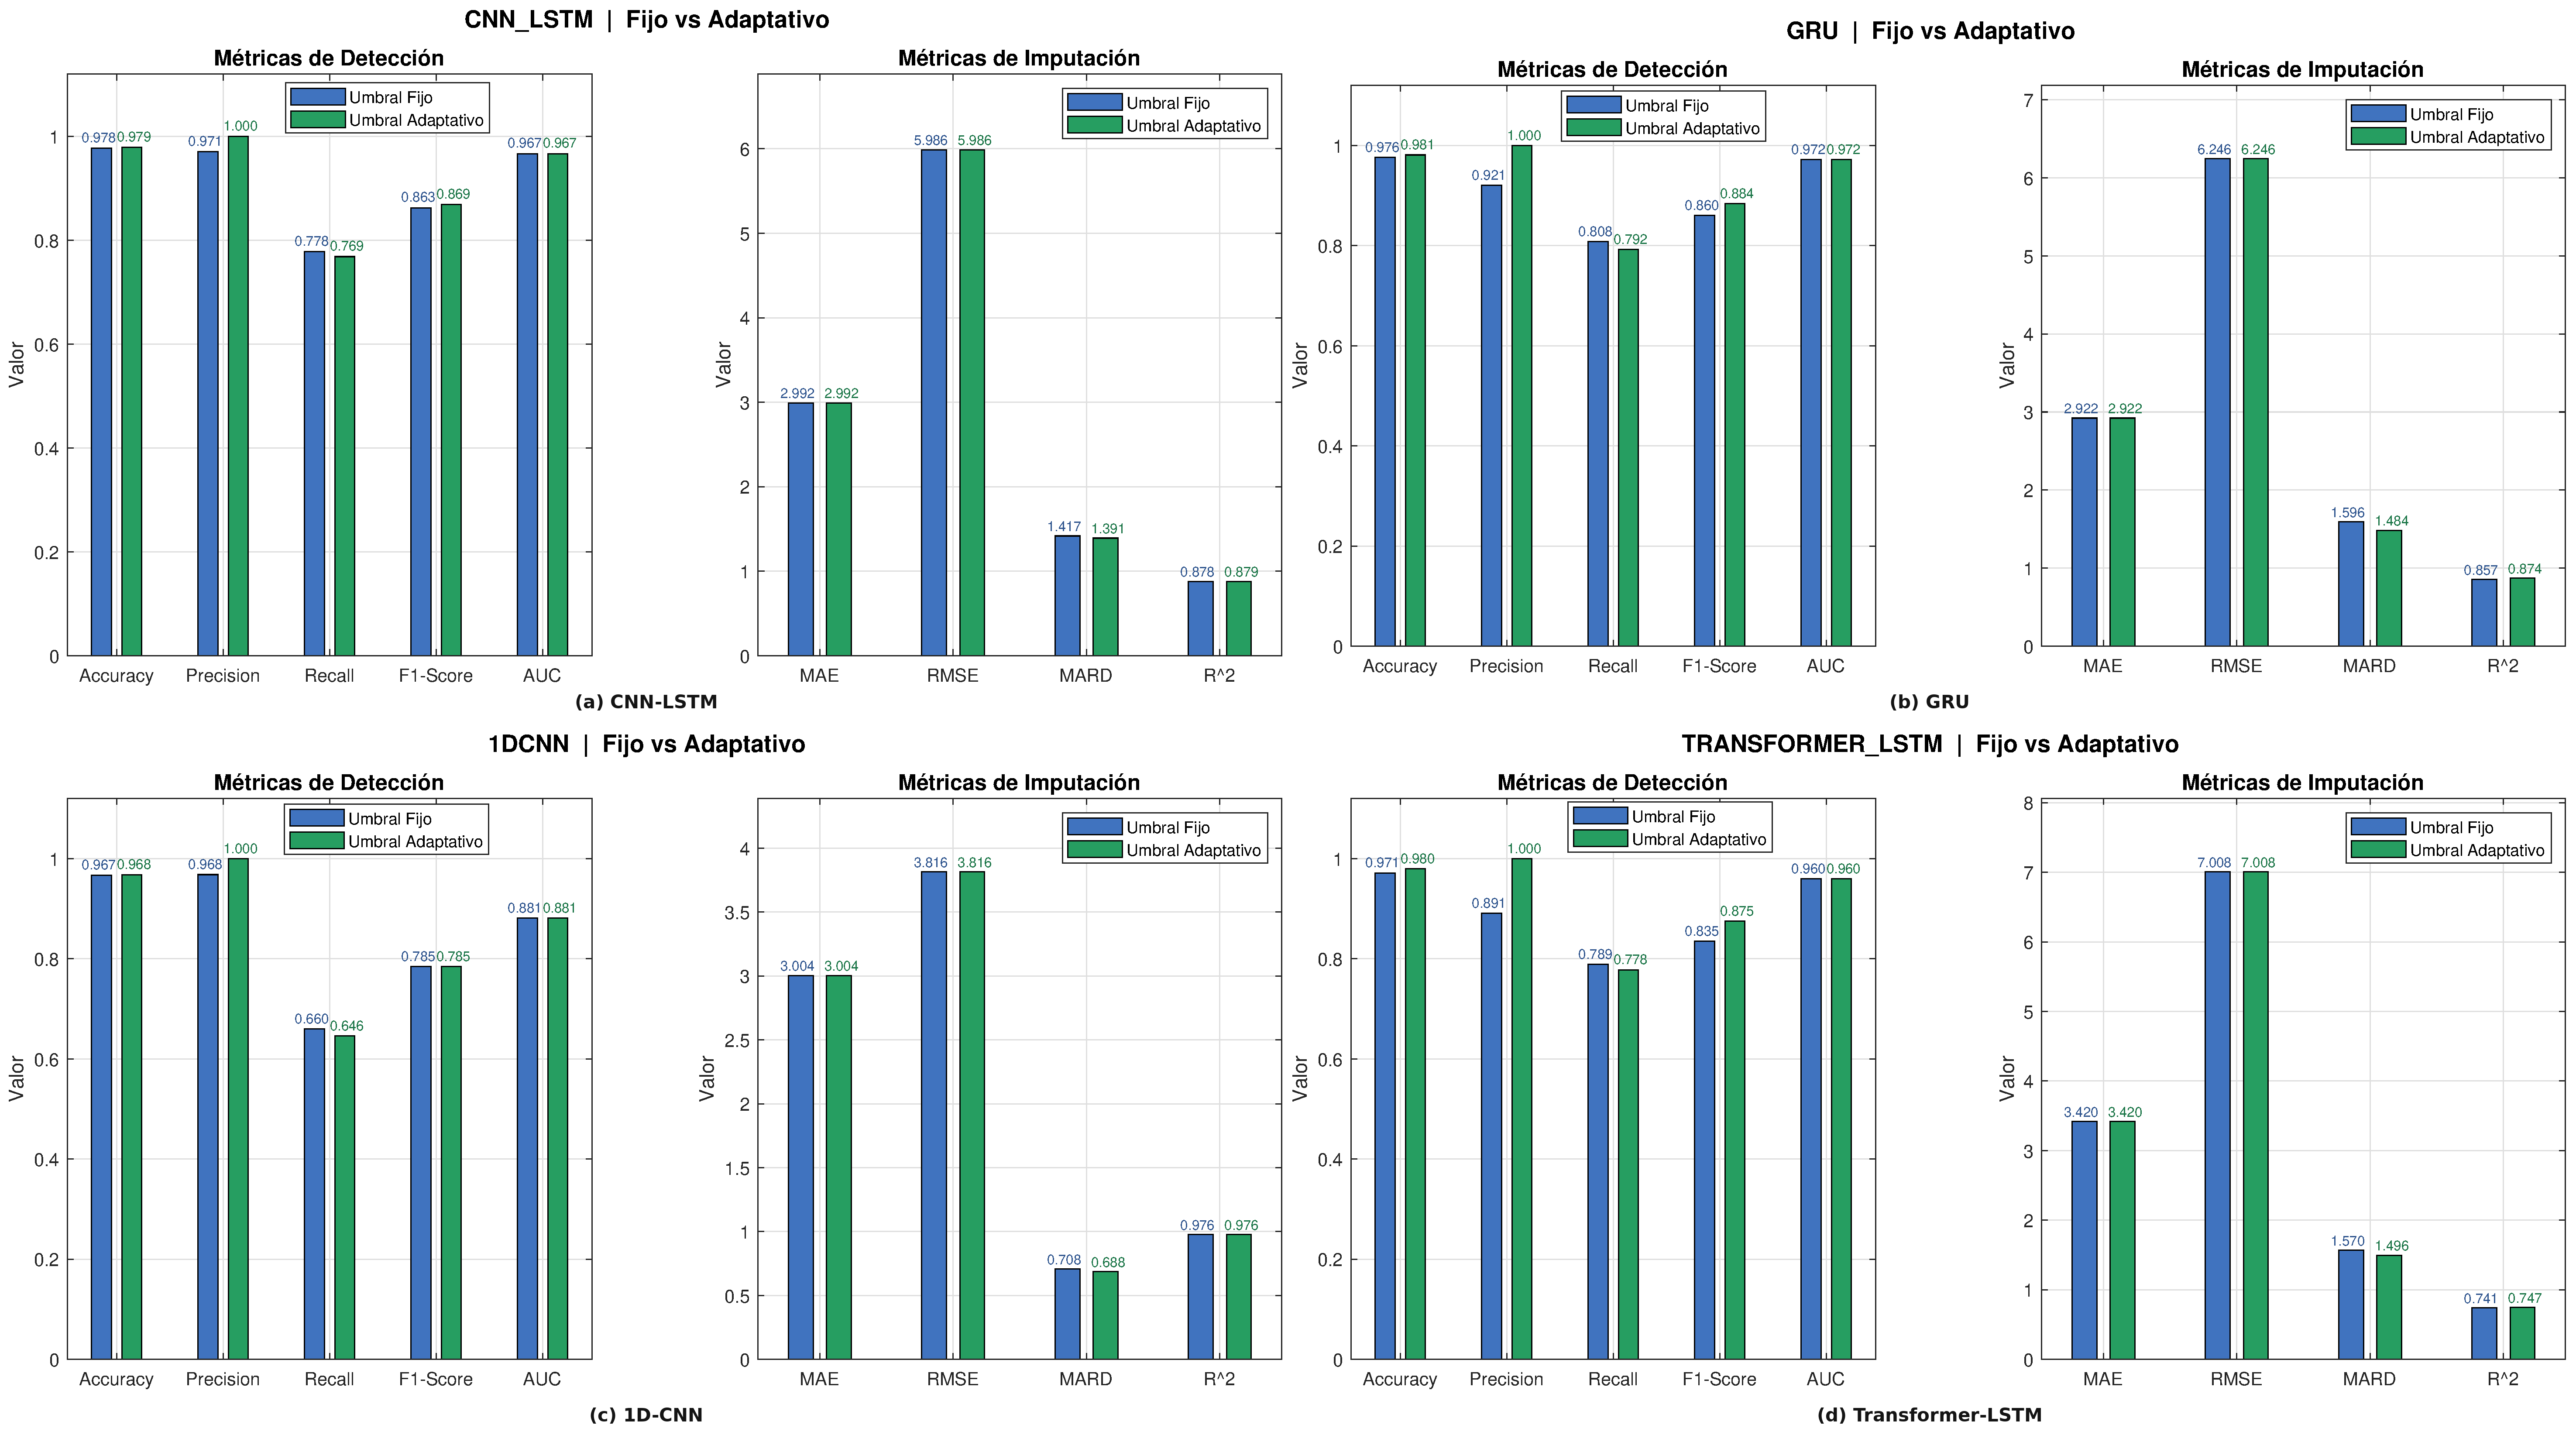
\includegraphics[width=\textwidth]{figures/figura_comparativa_fijo_vs_adaptativo.png}
% \caption{Comparación de métricas de detección e imputación entre umbral fijo 
%          ($\tau = 10$\,mg/dL) y umbral adaptativo para las cuatro arquitecturas 
%          evaluadas: (a) CNN-LSTM, (b) GRU, (c) 1D-CNN y (d) Transformer-LSTM.}
% \label{fig:comparativa_fijo_adaptativo}
% \end{figure}

Las Tablas~\ref{tab:bloque_b_deteccion} y~\ref{tab:bloque_b_imputacion}
presentan las métricas de detección e imputación bajo el umbral adaptativo,
manteniendo el mismo formato que las tablas de la sección anterior para
facilitar la comparación visual.

% ------ Tabla detección ------
\begin{table}[htbp]
\centering
\caption{Métricas de detección de fallos — pipeline unificado con umbral
         adaptativo ($\beta=0.10$, $\tau_{\min}=7.0$\,mg/dL, $\gamma=0.05$).
         Valores expresados como media $\pm$ std sobre cinco semillas.}
\label{tab:bloque_b_deteccion}
\begin{tabular}{lrrrrr}
\toprule
\textbf{Arquitectura} &
\textbf{Accuracy} & \textbf{Precision} & \textbf{Recall} &
\textbf{F1-score} & \textbf{AUC} \\
\midrule
CNN-LSTM         & $0.979 \pm 0.003$ & $1.000 \pm 0.000$ & $0.769 \pm 0.027$
                 & $0.869 \pm 0.017$ & $0.967 \pm 0.012$ \\
GRU              & $0.981 \pm 0.001$ & $1.000 \pm 0.000$ & $0.792 \pm 0.012$
                 & $0.884 \pm 0.007$ & $0.972 \pm 0.005$ \\
1D-CNN           & $0.968 \pm 0.001$ & $1.000 \pm 0.000$ & $0.646 \pm 0.010$
                 & $0.785 \pm 0.007$ & $0.882 \pm 0.027$ \\
Transformer-LSTM & $0.980 \pm 0.002$ & $1.000 \pm 0.000$ & $0.778 \pm 0.017$
                 & $0.875 \pm 0.011$ & $0.960 \pm 0.013$ \\
\bottomrule
\end{tabular}
\end{table}

% ------ Tabla imputación ------
\begin{table}[htbp]
\centering
\caption{Métricas de imputación — pipeline unificado con umbral adaptativo.
         Valores expresados como media $\pm$ std sobre cinco semillas.
         MAE y RMSE en mg/dL; MARD en \%; $R^2$ adimensional.}
\label{tab:bloque_b_imputacion}
\begin{tabular}{lrrrr}
\toprule
\textbf{Arquitectura} &
\textbf{MAE} & \textbf{RMSE} & \textbf{MARD (\%)} & $\boldsymbol{R^2}$ \\
\midrule
CNN-LSTM         & $2.99 \pm 0.63$ & $5.99 \pm 1.75$ & $1.39 \pm 0.41$
                 & $0.879 \pm 0.077$ \\
GRU              & $2.92 \pm 0.26$ & $6.25 \pm 0.85$ & $1.48 \pm 0.19$
                 & $0.874 \pm 0.040$ \\
1D-CNN           & $3.00 \pm 0.51$ & $3.82 \pm 0.44$ & $0.69 \pm 0.023$
                 & $0.976 \pm 0.003$ \\
Transformer-LSTM & $3.42 \pm 1.44$ & $7.01 \pm 5.68$ & $1.50 \pm 1.27$
                 & $0.748 \pm 0.464$ \\
\bottomrule
\end{tabular}
\end{table}

\subsection*{Efecto sobre la detección}

El resultado más destacado del umbral adaptativo es la eliminación completa de los falsos positivos: las cuatro arquitecturas alcanzan una precisión de $1.000 \pm 0.000$ de forma consistente en todas las semillas evaluadas. Este comportamiento se debe a que el umbral $\tau(k)$ se escala con el nivel de glucosa predicho $\hat{g}(k)$ y con la tasa de cambio $|\text{ROC}(k)|$, adaptándose al contexto glucémico instantáneo. En regiones de glucosa elevada o con dinámica rápida —donde el error de predicción es intrínsecamente mayor aún en ausencia de fallo— el umbral se amplía proporcionalmente, evitando clasificar variaciones fisiológicas normales como anomalías del sensor.

Este efecto contrasta con el umbral fijo, cuyo valor constante de $10$\,mg/dL resulta demasiado restrictivo en determinados contextos glucémicos, generando falsos positivos que se traducen en precisiones inferiores a la unidad (entre $0.891$ y $0.971$ según la arquitectura, véase Tabla~\ref{tab:bloque_a_deteccion}).

Como contrapartida esperada, el recall disminuye levemente en todas las arquitecturas (entre $0.009$ y $0.016$ puntos), dado que un umbral más exigente puede dejar sin detectar algunos fallos de menor magnitud relativa. Sin embargo, el balance neto medido por el F1-score es favorable en tres de las cuatro arquitecturas: GRU pasa de $0.860$ a $0.884$ ($\Delta = +0.024$), Transformer-LSTM de $0.835$ a $0.875$ ($\Delta = +0.040$) y CNN-LSTM de $0.863$ a $0.869$ ($\Delta = +0.006$). Únicamente 1D-CNN mantiene su F1-score en $0.785$, sin cambio apreciable, lo que es consistente con su perfil conservador: al tener el recall más bajo desde el inicio, la ganancia en precisión no alcanza a compensar la pequeña pérdida adicional de sensibilidad.

El AUC permanece idéntico al del umbral fijo en todas las arquitecturas ($0.967$, $0.972$, $0.882$ y $0.960$, respectivamente). Este resultado es metodológicamente esperable: el AUC se calcula a partir del error de predicción continuo como puntuación discriminante, y es invariante respecto al umbral de binarización empleado. Su invarianza confirma que el umbral adaptativo no modifica la capacidad discriminativa intrínseca de los modelos, sino únicamente el punto de operación sobre la curva ROC.

La reducción de la dispersión en precisión del Transformer-LSTM ($\sigma: 0.089 \to 0.000$) merece una mención particular: bajo el umbral fijo, distintas semillas de este modelo producían tasas de falsos positivos considerablemente distintas entre sí, lo que se reflejaba en una alta varianza en precisión. El umbral adaptativo elimina esta variabilidad, homogeneizando el comportamiento de detección independientemente de la inicialización.

\subsection*{Efecto sobre la imputación}

Las métricas MAE y RMSE son idénticas a las del umbral fijo en todas las arquitecturas. Este resultado es consecuencia directa del diseño del pipeline unificado: el umbral únicamente determina si una muestra se clasifica como fallo o no; el valor imputado —cuando se activa la imputación— es siempre la predicción $\hat{g}(k)$ del modelo, independientemente de qué umbral la activó. Por tanto, cualquier muestra que era correctamente imputada bajo el umbral fijo lo sigue siendo bajo el umbral adaptativo, y viceversa.

El MARD, sin embargo, mejora de forma consistente en todas las arquitecturas (GRU: $-0.111$\,pp; Transformer-LSTM: $-0.074$\,pp; CNN-LSTM: $-0.026$\,pp; 1D-CNN: $-0.020$\,pp). Esta mejora, aparentemente contradictoria con la invarianza de MAE y RMSE, se explica por la naturaleza relativa del MARD: al eliminarse los falsos positivos, el sistema ya no imputa muestras que en realidad son correctas, evitando así introducir sustituciones en regiones de glucosa baja donde el error relativo es mayor. El efecto es sutil pero sistemático y consistente en las cuatro arquitecturas.

\subsection*{Rol del componente de tasa de cambio}

El parámetro $\gamma = 0.05$, que pondera la contribución de $|\text{ROC}(k)|$ al umbral, fue validado comparando su comportamiento frente a $\gamma = 0.00$ (umbral sin componente de tasa de cambio). En el  caso $\gamma = 0.00$, el umbral se reduce a $\tau(k) = \tau_{\min} + \beta \cdot \hat{g}(k)$, proporcional únicamente al nivel de glucosa, lo que reintroduce falsos positivos en transiciones glucémicas rápidas —como las ocurridas durante episodios postprandiales— donde el error de predicción aumenta transitoriamente sin que exista un fallo real del sensor. La inclusión del término $\gamma \cdot |\text{ROC}(k)|$ amplía el umbral precisamente en estos instantes, confirmando que la componente de tasa de cambio es esencial para alcanzar la precisión unitaria de forma robusta.

\subsection*{Síntesis comparativa}

El umbral adaptativo mejora de forma sistemática el perfil de detección del pipeline unificado sin degradar las métricas de imputación. La ganancia principal es la eliminación completa de falsos positivos, con una pérdida marginal de recall que el F1-score absorbe favorablemente en la mayoría de las arquitecturas. Estos resultados validan la hipótesis de diseño del umbral adaptativo y justifican su adopción como configuración estándar en todas las evaluaciones subsecuentes de esta tesis, incluyendo el pipeline desacoplado presentado en la Sección~\ref{sec:pipeline_desacoplado}.


%\section{Resultados de imputación de las 4 arquitecturas} % (paper sec. 5.1)
% =====================================================================
%  Sección 4.4 — Pipeline desacoplado: análisis de las 16 combinaciones
%  Requiere en el preámbulo: booktabs, caption (labelfont=bf),
%  \addto\captionsspanish{\renewcommand{\tablename}{Tabla}}
%  Numeración de tablas automática por capítulo (Tabla 4.X).
%  La figura fig_44_frente_pareto.eps se genera aparte (pendiente).
% =====================================================================

\section{Pipeline desacoplado: análisis de las 16 combinaciones}
\label{sec:pipeline-desacoplado}

En las secciones~\ref{sec:pipeline_unificado_fijo} y~\ref{sec:pipeline_unificado_adaptativo} el detector y el imputador compartían arquitectura, configuración a la que denominamos \emph{pipeline unificado}. Esta sección elimina dicha restricción: cada una de las cuatro arquitecturas puede desempeñar el rol de detector y, de forma independiente, el rol de imputador, dando lugar a las $4\times 4 = 16$ combinaciones del \emph{pipeline desacoplado}. El análisis persigue dos objetivos. Primero, verificar empíricamente la hipótesis de desacoplamiento, es decir, que el desempeño de detección y el de imputación son atribuibles a módulos distintos y no interactúan entre sí. Segundo, determinar si desacoplar ambos módulos aporta una ventaja frente al esquema unificado, que en este pipeline corresponde a la diagonal (detector = imputador).

Las métricas de imputación se reportan bajo la definición~D1, $|\hat{y}_{\text{imp}} - g_{\text{real}}|$ evaluada en \emph{todas} las muestras, idéntica a la empleada en esquema unificado con umbral adaptativo (Sección~\ref{sec:pipeline_unificado_adaptativo}) y en el trabajo publicado de referencia; esto garantiza la comparabilidad entre secciones. De forma complementaria se incluye la métrica~D3, $|g_{\text{final}} - g_{\text{real}}|$ restringida a las muestras con fallo real inyectado ($\texttt{true\_f}=1$), como métrica \emph{diagnóstica} de la calidad de reconstrucción justo donde la imputación actúa. La métrica~D3 no es comparable con el trabajo de referencia, que reporta~D1, y se presenta únicamente con fines de análisis.

\subsection{Independencia entre detección e imputación}
\label{subsec:independencia}

El resultado central de esta sección es la confirmación empírica \emph{exacta} de la independencia entre ambos módulos. En la Tabla~\ref{tab:44-f1}, las cuatro columnas de cada fila son idénticas: el $F_1$ de detección depende exclusivamente de la arquitectura del detector y es completamente insensible a qué imputador se acople. De forma simétrica, en la Tabla~\ref{tab:44-mae-d1} las cuatro filas son idénticas: el MAE de imputación depende exclusivamente del imputador. La misma estructura fila-idéntica se observa en el RMSE (Tabla~\ref{tab:44-rmse-d1}). En otras palabras, el error de detección y el error de imputación se factorizan por completo, lo que valida de manera directa la hipótesis de desacoplamiento y justifica tratar el diseño del detector y del imputador como problemas separables.

\begin{table}[htbp]
\centering
\caption{$F_1$ de detección para las 16 combinaciones. Las cuatro columnas de cada fila son idénticas: el desempeño de detección depende únicamente del detector. Valores como media $\pm$ desviación estándar.}
\label{tab:44-f1}
\small
\begin{tabular}{lcccc}
\toprule
 & \multicolumn{4}{c}{\textbf{Imputador}} \\
\cmidrule(lr){2-5}
\textbf{Detector} & CNN-LSTM & GRU & 1D-CNN & Transformer-LSTM \\
\midrule
CNN-LSTM          & $0.869 \pm 0.017$ & $0.869 \pm 0.017$ & $0.869 \pm 0.017$ & $0.869 \pm 0.017$ \\
GRU               & $0.884 \pm 0.007$ & $0.884 \pm 0.007$ & $0.884 \pm 0.007$ & $0.884 \pm 0.007$ \\
1D-CNN            & $0.785 \pm 0.007$ & $0.785 \pm 0.007$ & $0.785 \pm 0.007$ & $0.785 \pm 0.007$ \\
Transformer-LSTM  & $0.875 \pm 0.011$ & $0.875 \pm 0.011$ & $0.875 \pm 0.011$ & $0.875 \pm 0.011$ \\
\bottomrule
\end{tabular}
\end{table}

\begin{table}[htbp]
\centering
\caption{MAE de imputación (D1, mg/dL) para las 16 combinaciones. Las cuatro filas son idénticas: el error de imputación depende únicamente del imputador. Valores como media $\pm$ desviación estándar.}
\label{tab:44-mae-d1}
\small
\begin{tabular}{lcccc}
\toprule
 & \multicolumn{4}{c}{\textbf{Imputador}} \\
\cmidrule(lr){2-5}
\textbf{Detector} & CNN-LSTM & GRU & 1D-CNN & Transformer-LSTM \\
\midrule
CNN-LSTM          & $3.00 \pm 0.64$ & $2.92 \pm 0.26$ & $3.00 \pm 0.51$ & $3.43 \pm 1.47$ \\
GRU               & $3.00 \pm 0.64$ & $2.92 \pm 0.26$ & $3.00 \pm 0.51$ & $3.43 \pm 1.47$ \\
1D-CNN            & $3.00 \pm 0.64$ & $2.92 \pm 0.26$ & $3.00 \pm 0.51$ & $3.43 \pm 1.47$ \\
Transformer-LSTM  & $3.00 \pm 0.64$ & $2.92 \pm 0.26$ & $3.00 \pm 0.51$ & $3.43 \pm 1.47$ \\
\bottomrule
\end{tabular}
\end{table}

Conviene ser preciso respecto al alcance de esta independencia. Es \emph{exacta} en las tres métricas anteriores ($F_1$, MAE y RMSE bajo~D1), donde las tablas son idénticas por fila o por columna. En cambio, en el coeficiente de determinación~$R^2$ (Tabla~\ref{tab:44-r2}), en el MARD (Tabla~\ref{tab:44-mard}) y en la métrica diagnóstica~D3 (Tabla~\ref{tab:44-mae-d3}) se observa una dependencia \emph{residual} del detector: estas métricas se calculan sobre la señal de salida $g_{\text{final}}$ o sobre el subconjunto de muestras válidas, cuya composición varía marginalmente según las muestras que cada detector señale. La variación afecta a la tercera o cuarta cifra decimal y no altera ninguno de los ordenamientos, por lo que la conclusión de independencia se mantiene en la práctica para todas las métricas.

\subsection{Desempeño del detector}
\label{subsec:detector-f1}

El ordenamiento de detectores según $F_1$ (Tabla~\ref{tab:44-f1}) es:
GRU ($0.884 \pm 0.007$), seguido de Transformer-LSTM ($0.875 \pm 0.011$),
CNN-LSTM ($0.869 \pm 0.017$) y, con una diferencia apreciable, 1D-CNN
($0.785 \pm 0.007$). Las cuatro arquitecturas mantienen una precisión de $1.000$ (cero falsos positivos), propiedad ya validada en la Sección~\ref{sec:pipeline_unificado_adaptativo} como consecuencia del umbral adaptativo; las diferencias en $F_1$ provienen por tanto íntegramente de la sensibilidad (recall). GRU ofrece el mejor compromiso de detección, mientras que 1D-CNN, pese a su solvencia como imputador (Sección~\ref{subsec:imputador}), es el detector más débil.

\subsection{Desempeño del imputador}
\label{subsec:imputador}

El análisis del imputador revela un compromiso claro entre dos perfiles. GRU alcanza el menor MAE ($2.92 \pm 0.26$~mg/dL, Tabla~\ref{tab:44-mae-d1}), es decir, el mejor error absoluto puro. 1D-CNN, en cambio, domina el ajuste global: obtiene el menor RMSE ($3.82 \pm 0.44$~mg/dL, Tabla~\ref{tab:44-rmse-d1}), el mayor $R^2$ ($0.975$–$0.980$, Tabla~\ref{tab:44-r2}) y el menor MARD ($0.66$–$0.69$\,\%, Tabla~\ref{tab:44-mard}). CNN-LSTM presenta un MAE comparable ($3.00 \pm 0.64$) pero un RMSE elevado ($6.00 \pm 1.78$) y un $R^2$ moderado ($\approx 0.88$), con mayor varianza. Transformer-LSTM es el peor imputador en todas las métricas (MAE $3.43 \pm 1.47$, RMSE $7.04 \pm 5.75$, $R^2 \approx 0.74$–$0.75$); su elevada desviación estándar es coherente con la inestabilidad de entrenamiento documentada en la Sección~\ref{sec:resultados_entrenamiento}.

El contraste entre MAE y RMSE es informativo. GRU minimiza el MAE pero no el RMSE, lo que indica errores pequeños y frecuentes acompañados de algunos errores grandes; 1D-CNN, con el menor RMSE, se comporta de forma más consistente y penaliza menos los casos atípicos. Esta distinción es la base del compromiso entre configuraciones que se discute en la Sección~\ref{subsec:co-optimas}.

\begin{table}[htbp]
\centering
\caption{RMSE de imputación (D1, mg/dL) para las 16 combinaciones. Filas idénticas: depende únicamente del imputador. Valores como media $\pm$ desviación estándar.}
\label{tab:44-rmse-d1}
\small
\begin{tabular}{lcccc}
\toprule
 & \multicolumn{4}{c}{\textbf{Imputador}} \\
\cmidrule(lr){2-5}
\textbf{Detector} & CNN-LSTM & GRU & 1D-CNN & Transformer-LSTM \\
\midrule
CNN-LSTM          & $6.00 \pm 1.78$ & $6.25 \pm 0.85$ & $3.82 \pm 0.44$ & $7.04 \pm 5.75$ \\
GRU               & $6.00 \pm 1.78$ & $6.25 \pm 0.85$ & $3.82 \pm 0.44$ & $7.04 \pm 5.75$ \\
1D-CNN            & $6.00 \pm 1.78$ & $6.25 \pm 0.85$ & $3.82 \pm 0.44$ & $7.04 \pm 5.75$ \\
Transformer-LSTM  & $6.00 \pm 1.78$ & $6.25 \pm 0.85$ & $3.82 \pm 0.44$ & $7.04 \pm 5.75$ \\
\bottomrule
\end{tabular}
\end{table}

\begin{table}[htbp]
\centering
\caption{Coeficiente de determinación $R^2$ (sobre la señal de salida $g_{\text{final}}$) para las 16 combinaciones. Se aprecia una dependencia residual del detector en la tercera cifra decimal, sin efecto sobre el ordenamiento.}
\label{tab:44-r2}
\small
\begin{tabular}{lcccc}
\toprule
 & \multicolumn{4}{c}{\textbf{Imputador}} \\
\cmidrule(lr){2-5}
\textbf{Detector} & CNN-LSTM & GRU & 1D-CNN & Transformer-LSTM \\
\midrule
CNN-LSTM          & $0.8798$ & $0.8790$ & $0.9801$ & $0.7516$ \\
GRU               & $0.8776$ & $0.8753$ & $0.9787$ & $0.7426$ \\
1D-CNN            & $0.8749$ & $0.8734$ & $0.9752$ & $0.7439$ \\
Transformer-LSTM  & $0.8758$ & $0.8741$ & $0.9752$ & $0.7469$ \\
\bottomrule
\end{tabular}
\end{table}

\begin{table}[htbp]
\centering
\caption{MARD de imputación (D1, \%). Dependencia residual del detector por la exclusión de muestras con $g_{\text{real}} < 20$~mg/dL, cuyo conjunto varía marginalmente según el detector.}
\label{tab:44-mard}
\small
\begin{tabular}{lcccc}
\toprule
 & \multicolumn{4}{c}{\textbf{Imputador}} \\
\cmidrule(lr){2-5}
\textbf{Detector} & CNN-LSTM & GRU & 1D-CNN & Transformer-LSTM \\
\midrule
CNN-LSTM          & $1.38$ & $1.43$ & $0.66$ & $1.45$ \\
GRU               & $1.39$ & $1.46$ & $0.67$ & $1.48$ \\
1D-CNN            & $1.40$ & $1.46$ & $0.69$ & $1.48$ \\
Transformer-LSTM  & $1.40$ & $1.47$ & $0.70$ & $1.49$ \\
\bottomrule
\end{tabular}
\end{table}

\subsection{Reconstrucción en fallos reales (métrica diagnóstica)}
\label{subsec:d3}

La métrica~D3 (Tabla~\ref{tab:44-mae-d3}) evalúa el error de la señal de salida únicamente en las muestras con fallo real, aislando la calidad de reconstrucción del promediado con las muestras limpias. El resultado refuerza el hallazgo anterior: 1D-CNN reconstruye con un error de $5.2$–$5.7$~mg/dL, frente a los $13$–$14.5$~mg/dL del resto de imputadores. Esta ventaja de aproximadamente un factor de tres es coherente con su $R^2$ superior y confirma que 1D-CNN es el imputador que mejor recupera la señal justo donde la imputación es necesaria. Se reitera que~D3 se emplea como métrica diagnóstica y no como cifra comparable con el trabajo de referencia.

\begin{table}[htbp]
\centering
\caption{MAE de reconstrucción (D3, mg/dL) sobre las muestras con fallo real
($\texttt{true\_f}=1$). Métrica diagnóstica. Valores como media $\pm$ desviación
estándar.}
\label{tab:44-mae-d3}
\small
\begin{tabular}{lcccc}
\toprule
 & \multicolumn{4}{c}{\textbf{Imputador}} \\
\cmidrule(lr){2-5}
\textbf{Detector} & CNN-LSTM & GRU & 1D-CNN & Transformer-LSTM \\
\midrule
CNN-LSTM          & $13.33 \pm 4.82$ & $14.03 \pm 2.09$ & $5.24 \pm 0.31$ & $14.07 \pm 14.34$ \\
GRU               & $13.46 \pm 4.84$ & $14.33 \pm 2.06$ & $5.37 \pm 0.36$ & $14.49 \pm 14.88$ \\
1D-CNN            & $13.63 \pm 4.69$ & $14.41 \pm 2.41$ & $5.61 \pm 0.35$ & $14.54 \pm 14.36$ \\
Transformer-LSTM  & $13.63 \pm 4.71$ & $14.50 \pm 2.32$ & $5.73 \pm 0.91$ & $14.57 \pm 14.84$ \\
\bottomrule
\end{tabular}
\end{table}

\subsection{Configuraciones co-óptimas}
\label{subsec:co-optimas}

El análisis anterior no arroja un único ganador, sino dos configuraciones no dominadas que comparten el mejor detector (GRU) y se distinguen por el criterio de imputación priorizado:

\begin{itemize}
  \item \textbf{GRU\,$\rightarrow$\,GRU}: mejor $F_1$ de detección ($0.884$) y menor MAE de imputación ($2.92$~mg/dL). Recomendada cuando se prioriza el error absoluto.
  \item \textbf{GRU\,$\rightarrow$\,1D-CNN}: mejor $F_1$ de detección ($0.884$) junto con el mejor RMSE ($3.82$~mg/dL), el mejor $R^2$ ($0.9787$) y el mejor D3 ($5.37$~mg/dL).   Recomendada cuando se prioriza la calidad de reconstrucción global.
\end{itemize}

La elección entre ambas depende del objetivo clínico: minimizar el error medio favorece GRU\,$\rightarrow$\,GRU, mientras que privilegiar la fidelidad de la señal reconstruida y la robustez frente a errores grandes favorece GRU\,$\rightarrow$\,1D-CNN. La Figura~\ref{fig:44-frente} sitúa las 16 combinaciones en el plano detección–imputación y resalta ambas configuraciones.

\begin{figure}[htbp]
\centering
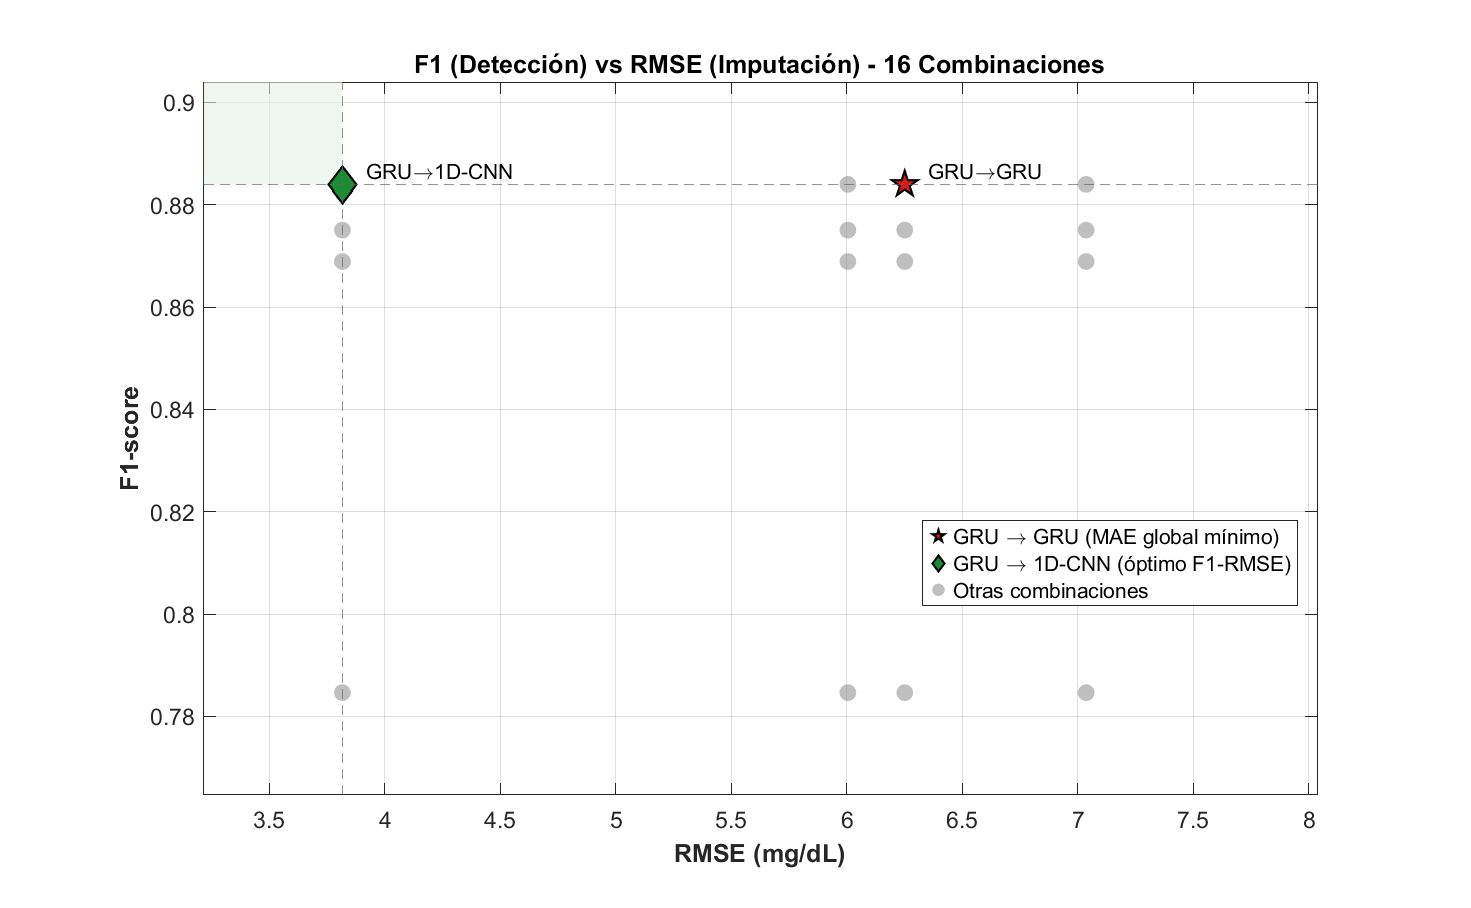
\includegraphics[width=\textwidth]{figures/fig_4_4_pareto_F1_RMSE.eps}
\caption{Las 16 combinaciones detector\,$\times$\,imputador en el plano $F_1$ (detección) frente a MAE (imputación, D1). La estructura de rejilla evidencia la independencia entre módulos. Se resaltan las configuraciones co-óptimas GRU\,$\rightarrow$\,GRU y GRU\,$\rightarrow$\,1D-CNN.}
\label{fig:44-frente}
\end{figure}

\subsection{Comparación con el esquema unificado}
\label{subsec:diagonal-vs-desacoplado}

La diagonal del pipeline desacoplado (detector = imputador) reproduce el esquema unificado de la Sección~\ref{sec:pipeline_unificado_adaptativo}. Al comparar cada detector con su mejor imputador posible, la reducción de MAE que aporta desacoplar es modesta: no supera el 15\,\% y en varios casos es inferior al 3\,\%. El mayor beneficio corresponde a Transformer-LSTM como detector, que pasa de $3.43$~mg/dL con su propio imputador a $2.92$~mg/dL al acoplarle GRU ($\approx 15$\,\%); para CNN-LSTM y 1D-CNN la mejora es de apenas $\approx 3$\,\%, y para GRU es nula, pues su propio imputador ya minimiza el MAE.

Sin embargo, reducir el MAE no es el aporte principal del desacoplamiento. Su valor real reside en desligar la elección del detector de la del imputador, ampliando el espacio de diseño del sistema. El caso más ilustrativo es GRU\,$\rightarrow$\,1D-CNN: el esquema unificado no puede acceder a la calidad de reconstrucción de 1D-CNN (RMSE $3.82$, $R^2 \approx 0.98$, D3 $\approx 5.4$~mg/dL) sin usarlo también como detector, lo que obliga a aceptar el peor $F_1$ ($0.785$). El pipeline desacoplado rompe esa atadura y permite combinar el mejor detector (GRU, $F_1 = 0.884$) con el mejor imputador de reconstrucción (1D-CNN), una configuración inalcanzable en el esquema unificado. Este es el argumento central a favor del desacoplamiento: más que optimizar una métrica puntual, habilita combinaciones de diseño que el esquema unificado excluye por construcción. 

\section{Resultados de detección de fallos} % (paper sec. 5.2)
\section{Comparación contra ARIMA y TCN} %(paper)
\section{Validación del umbral adaptativo} % las 16 combinaciones, eliminación de falsos positivos, β·ROC
\section{Pipeline integrado 4×4: análisis de las 16 combinaciones} % (co-óptimos GRU→1D-CNN y CNN-LSTM→1D-CNN
\section{Validación clínica e impacto sobre indicadores TIR/hipo/hiper}
\section{Validación en datos reales OhioT1DM}

% =================================================
% CAPÍTULO 5. DISCUSIÓN
% =================================================
\chapter{Discusión}

\section{Hallazgos principales y comparación con el estado del arte}
\section{Trade-off precisión–recall del umbral adaptativo: justificación clínica}
\section{Implicaciones clínicas: por qué los falsos positivos importan en CGM}
\section{Limitaciones (un solo paciente real, generalización, costo computacional)}

% =================================================
% CAPÍTULO 6. CONCLUSIONES
% =================================================
\chapter{Conclusiones y trabajo a futuro}

\section{Conclusiones generales}
\section{Aportaciones específicas de la tesis}
\section{Trabajo futuro (más pacientes OhioT1DM, lazo cerrado, dispositivo embebido}

%\section{Referencias}

\bibliographystyle{ieeetr}
\bibliography{samples}

\end{document}
